% Rewritten manuscript through methodology, with complete mathematical appendix.
% Compile with: pdflatex main.tex (twice).
% Uses the official ICLR 2027 style if supplied by the authors.
% The bundled fallback is a reading layout, not a certified conference template.
\documentclass[10pt]{article}
\newif\ifofficialstyle
\IfFileExists{iclr2027_conference.sty}{\officialstyletrue\usepackage{iclr2027_conference}}{%
  \officialstylefalse
  \usepackage[letterpaper,textwidth=5.5in,textheight=9in,centering]{geometry}
  \usepackage{natbib}
  \usepackage{fancyhdr}
  \pagestyle{fancy}\fancyhf{}
  \fancyhead[C]{\small Topological Self-Regulation in Neural Networks}
  \fancyfoot[C]{\thepage}
  \renewcommand{\headrulewidth}{0pt}
  \setlength{\headheight}{14pt}
}
\usepackage[T1]{fontenc}
\usepackage{times}
\usepackage{amsmath,amssymb,amsthm,bm}
\usepackage{microtype}
\setlength{\emergencystretch}{1em}
\usepackage{booktabs,array}
\usepackage{graphicx}
\usepackage[font=footnotesize,labelfont=bf,skip=4pt]{caption}
\usepackage[hidelinks]{hyperref}
\hypersetup{pdftitle={Topological Self-Regulation in Neural Networks},pdfauthor={Anonymous authors}}
\usepackage[nameinlink,noabbrev]{cleveref}
\setcitestyle{authoryear,round}
\newtheoremstyle{paper}{6pt}{6pt}{\normalfont}{} {\bfseries}{.}{.5em}{}
\theoremstyle{paper}
\newtheorem{theorem}{Theorem}[section]
\newtheorem{proposition}[theorem]{Proposition}
\newtheorem{lemma}[theorem]{Lemma}
\newtheorem{corollary}[theorem]{Corollary}
\newcommand{\R}{\mathbb R}
\newcommand{\E}{\mathbb E}
\newcommand{\Prob}{\mathbb P}
\newcommand{\Lcal}{\mathcal L}
\newcommand{\Sset}{\mathcal S}
\newcommand{\norm}[1]{\left\lVert #1\right\rVert}
\newcommand{\wc}{w_c}
\newcommand{\uc}{u_c}
\newcommand{\vc}{v_c}
\newcommand{\ip}[2]{\left\langle #1,#2\right\rangle}
\DeclareMathOperator*{\argmax}{arg\,max}
\DeclareMathOperator*{\argmin}{arg\,min}
\DeclareMathOperator{\Cov}{Cov}
\DeclareMathOperator{\diag}{diag}
\DeclareMathOperator{\sg}{sg}
\title{Topological Self-Regulation in Neural Networks}
\author{Anonymous authors}
\date{}
\begin{document}
\maketitle
\begin{abstract}
A neural network learns how to use its channels during training, but where those channels sit is decided before the first gradient is taken, by convention rather than by the task. One part of a network can be starved of channels while another carries channels it barely uses. We ask whether training itself can revise this allocation. Topological Self-Regulation (TSR) treats channel width as a budgeted, revisable part of the model: silent candidate channels are attached throughout the network, the ordinary backward pass reveals which of them would be worth introducing and which incumbents contribute least, and capacity is transferred between them through edits that keep every dependent tensor consistent. A coupling calculus makes such edits valid across residual trunks, depthwise stacks, normalization state and optimizer moments, and the deployed parameter count is computed exactly from the edited tensors. Across four image-classification families and four forecasting backbones, the discovered architectures match the dense reference at roughly fifteen percent fewer parameters in vision and at reductions reaching well over half the network in forecasting. On the convolutional and mixing forecasters, the task-directed allocation outperforms a random one of the same size, and pruning the same reference to the same count shows how much of that is reallocation rather than removal. A three-seed ablation locates the source of the allocation: disabling growth, or placing it at random, leaves the retrained architecture's accuracy unchanged, so its value lies in budgeted, removal-led reallocation rather than in gradient-directed growth, and the allocation itself is stable across seeds and controller settings.
\end{abstract}

\section{Introduction}
\label{sec:intro}
A network can learn how to use its channels without learning where those channels should be. Conventional widths are chosen before training, often by doubling channels after downsampling or imposing a fixed expansion ratio. Weights then adapt within that allocation, even when a useful feature cannot be expressed at one site and capacity at another contributes little. We ask whether the task loss can also guide a revision of the network's internal dimensions. This requires a connection between redundancy and opportunity. Removal asks what the network would lose, while growth asks what a proposed feature could contribute, which depends on how it enters the computation. We evaluate that opportunity through a candidate whose outgoing weights are zero. Its presence leaves the current function unchanged, yet the loss gradient at those weights need not vanish, and that gradient is the direction along which the feature would enter. The same sensitivity read at an incumbent recovers the activation-gradient product of Taylor pruning \citep{molchanov2017pruning}.

Topological Self-Regulation uses this connection to revise widths during a discovery run. Its contributions are a coupling calculus, an index representation that makes edits in both directions valid across every dependent tensor; a budgeted controller that revises widths inside a single training run; and a protocol that separates the value of an allocation from the run that found it. The protocol also tests the controller's own premise, and a growth ablation (\cref{sec:ablation}) finds that the allocation's value does not come from gradient-directed growth. Two levels are analyzed: the released controller reallocates capacity using gradient-derived surrogate scores, and a calibrated reference rule replaces those scores by loss-change bounds that admit a local descent certificate. That certificate belongs to the calibrated variant rather than to every practical edit.

Width allocation occupies a middle ground between post hoc pruning, which asks which components of a chosen architecture can be discarded \citep{han2015learning,li2016pruning,he2017channel}, and architecture search, which evaluates many designs under a separate search procedure or a proxy training budget \citep{zoph2017neural,liu2018darts,JMLR:v20:18-598}. TSR instead holds the computational skeleton fixed and lets training redistribute a prescribed resource among its editable groups. When a model family has already fixed its operators and its connectivity, can the task signal improve the allocation of channels inside that family? Asking it this way is what makes the comparison possible, against a dense reference and against the same discovered widths trained from scratch. That comparison also separates effects that dynamic-architecture results can otherwise confound. A compact network may be better because its widths are better allocated, or because its parameters took a particular sequence of edits and a different optimization trajectory. We therefore treat the online discovery run and the static retraining of its exported shape as different experimental objects, the first measuring what self-regulation costs during learning and the second asking whether the discovered allocation is valuable on its own. Structural validity and resource accounting carry as much weight here as the saliency rule does, as do the empirical controls.

\section{Related Work}
\label{sec:related}
\textbf{Growth and removal.} Cascade-Correlation learns candidate features from residual errors \citep{fahlman1989cascade}, Net2Net preserves a function while enlarging its parameterization \citep{Chen2016}, and GradMax uses gradient information to initialize new units \citep{evci2022gradmax}. TSR carries this perspective to candidate ports at interior sites and reads their sensitivity from the same backward pass as removal; its candidate objective is connected to covariance selection in \cref{app:candidates}. On the removal side, skeletonization and Taylor pruning measure the sensitivity of existing units \citep{mozer1988skeletonization,molchanov2017pruning}, curvature refines the linear estimate when trained gradients become small \citep{lecun1989optimal,hassibi1992second}, channel pruning removes dimensions from a trained network \citep{han2015learning,li2016pruning,he2017channel,liu2017learning}, DepGraph resolves the dependencies that constrain channel removal \citep{10204583}, and Isomorphic Pruning ranks each sub-structure only against structurally matching ones \citep{fang2024isomorphic}. Our coupling calculus extends that discipline to edits in both directions and to optimizer state.

\textbf{Structure changed during training.} Dynamic sparse training reallocates a mask over individual weights and leaves the ambient shapes alone \citep{evci2020rigging}; its structured form, SRigL, constrains the mask to whole neurons so the trained network can afterwards be condensed \citep{lasby2024dynamic}, and BilevelPruning learns a channel mask during training and applies it statically at the end \citep{gao2024bilevelpruning}. NeST grows connections and then prunes them in separate phases \citep{dai2019nest}, structured continuous sparsification grows widths under a joint accuracy and sparsity objective \citep{yuan2021growing}, incremental growth with variance transfer expands a small network during training to cut its cost \citep{yuan2023accelerated}, and \citet{swiderski2025growing} grow and shrink networks during training with structural decisions guided by Monte Carlo tree search. OTOv2 trains and structurally prunes a network in one run from scratch, over zero-invariant groups derived from its dependency graph, with a sparsity-inducing optimizer \citep{chen2023otov2}; it is the closest relative of removal-only TSR (\cref{sec:ablation}), which removes by a budgeted ranking instead and also admits growth. MorphNet and AutoSlim redistribute capacity within an architectural family through a resource regularizer or a slimmable supernetwork \citep{gordon2018morphnet,8822c3c89a3f4ee0bf3b01a679aabd6b,yu2020autoslim}. What separates TSR is what gets decided and from what evidence. A mask chooses which existing channels survive; TSR changes how many channels each site has, can put capacity where the reference had none, and edits every dependent tensor and optimizer state to match, with growth and removal read from one backward pass and spent against one budget. An unstructured sparsity result is therefore context rather than a control, and a structured mask controls the removal half of an exchange without its growth half. TSR also keeps a transparent correspondence between a discovered width vector and a retrainable static control, which is what lets the controls of \cref{sec:experiments} locate the source of an effect. \Cref{app:related} expands these comparisons.

\section{Structural Optimization}
\label{sec:problem}
\begin{figure}[t]
\centering
\includegraphics[width=\textwidth]{figures/methtsr.png}
\caption{\textbf{One structural update.} Every $T_{\mathrm{struct}} = 100$ optimizer steps the controller reads the current widths, prices every coupling group and applies one edit; $\theta$ trains continuously in between. \textbf{I}~the coupling groups, recovered by union--find over channel axes. \textbf{II}~the four admissibility tests a group must pass. \textbf{III}~growth sensed at dormant ports held at $\wc = 0$, removal saliency read at incumbents. \textbf{IV}~both divided by the marginal parameter cost $\kappa_\ell$. \textbf{V}~force-prune above the annealed budget $B(t)$, exchange below it. Only the task-fixed axes differ between forecasting and image classification.}
\label{fig:method}
\end{figure}

\Cref{fig:method} summarizes one structural update. Channels whose indices must change together, because a residual addition, a normalization layer or a consumer's input ties them, form a \emph{coupling group}, and only whole groups are resized. A group is editable when four tests pass (\cref{app:admissibility}): it has both a producer and a consumer; every normalizer over it computes per-channel statistics (Condition (N) below); no hard-coded reshape depends on its width (Condition (R)); and it is not fixed by the task, as the input and class dimensions are. For each editable group the controller reads two signals from the ordinary backward pass, a growth signal at \emph{candidate} channels that are attached but silent and a removal signal at \emph{incumbent} channels that already exist, divides each by the group's per-channel parameter cost $\kappa_\ell$, and moves capacity between groups under a budget. The rest of this section and \cref{sec:theory} define these quantities in order; \cref{tab:notation} collects the notation.

Let $\Sset$ index the editable coupling groups and collect their widths in a vector $\bm n$. The admissible set $\mathcal N$ contains the width vectors the architecture accepts, each width at or above a floor and consistent with the conditions of \cref{app:admissibility}, and $\theta\in\Theta(\bm n)$ are the weights of the network at widths $\bm n$. We consider
\begin{equation}
\min_{\bm n\in\mathcal N}\ \min_{\theta\in\Theta(\bm n)}
\Lcal(\theta,\bm n)\quad\text{subject to}\quad C(\bm n)\le B,
\label{eq:problem}
\end{equation}
where $\Lcal=\E[\ell(f_{\theta,\bm n}(x),y)]$, $C$ counts deployed parameters, and $B$ is the budget, a prescribed parameter count (any additive cost can take its place, \cref{app:flops}). The architecture skeleton and task dimensions remain fixed.

A coupling group $G$ carries an abstract index set $I_G$. Each occurrence $b$ of this index in a parameter or state tensor, such as a producer's output axis, a consumer's input axis, a normalization buffer or an optimizer moment, has a map $\rho_b:I_G\times\{1,\ldots,m_b\}\to\mathbb N$ to positions along that tensor's axis, where $m_b>1$ handles layouts in which one channel occupies several positions, such as a flattened spatial block. Residual addition identifies index sets, whereas concatenation preserves separate blocks and their offsets. An admissible edit changes $I_G$ through every represented map and respects divisibility, reshape, normalization, and task-interface constraints. Counting each shared parameter tensor once gives
\begin{equation}
C(\bm n)=\sum_T\prod_a d_{T,a}(\bm n),
\label{eq:main-cost}
\end{equation}
so the exact resource change is a finite difference of $C$, not necessarily a sum of isolated marginal costs. Cross terms occur when two edited groups index different axes of one tensor. The complete index calculus and its operator-specific limitations are developed in \cref{app:coupling}.

A candidate has incoming parameters $w_c$ and a \emph{port} $v_c$, its outgoing weights: every independent outgoing coordinate through which it can affect retained computation. An admissible silent embedding satisfies $f_{\theta,w_c,0}=f_\theta$. Consequently,
\begin{equation}
\nabla_\theta\Lcal(\theta,w_c,0)=\nabla_\theta\Lcal(\theta),
\qquad \nabla_{w_c}\Lcal(\theta,w_c,0)=0,
\label{eq:main-embedding}
\end{equation}
while $\nabla_{v_c}\Lcal$ need not vanish. Silence requires all paths from the candidate into retained outputs to be blocked, including statistical paths, which gives two architectural conditions. Condition (N): no normalizer may compute statistics that span the edited axis. Appending one value to $n$ shifts such a shared mean by $q/(n+1)$ and the variance by an $O(1/n)$ amount (\cref{eq:normstats}), so a zero port cannot stop LayerNorm \citep{ba2016layer} over the edited feature axis or ordinary GroupNorm \citep{wu2018group} from perturbing retained coordinates; per-channel BatchNorm and InstanceNorm \citep{ioffe2015batch,ulyanov2016instance} satisfy (N). Condition (R): the width must remain compatible with hard-coded reshapes, such as the head split of multi-head attention \citep{vaswani2017attention}. Here ``topological'' is used in the sense of the topological derivative of shape optimization \citep{sokolowski1999topological,novotny2012topological}: it refers to adjoining a graph coordinate and differentiating at its silent embedding, and it is not a coordinate-free graph invariant. When the original weights are stationary, a nonzero $u_c$ makes the silent embedding non-stationary and a vanishing $u_c$ with a nonzero mixed block makes it a strict saddle \citep{ge2015escaping} (\cref{prop:escape}). \Cref{app:embedding,app:admissibility} supply the proofs and the full analytic and architectural conditions.

\section{From Sensitivity to Reallocation}
\label{sec:theory}
Throughout, the \emph{sensitivity} of a channel is the gradient of the loss with respect to its port. At a silent candidate it is called the topological derivative,
\begin{equation}
u_c=\left.\nabla_{v_c}\Lcal(\theta,w_c,v_c)\right|_{v_c=0}.
\label{eq:derivative}
\end{equation}
A port coordinate $s$ can be used at several places in the computation; for a convolution, one weight is applied at every spatial position. Writing $\mathcal U_s$ for the set of those uses, and $a_{s,q}$ and $g_{s,q}$ for the activation entering use $q$ and the loss gradient leaving it, reverse-mode differentiation gives
\begin{equation}
(u_c)_s=\E\!\left[\sum_{q\in\mathcal U_s}a_{s,q}g_{s,q}\right].
\label{eq:main-port-uses}
\end{equation}
For a dense consumer this is $\E[a_cg]$. For a convolution, spatial products are summed at their aligned offsets before expectation. Pooling activations and adjoints separately would introduce incorrect cross-position products. Multiple independent consumers form blocks of one joint port, while contributions to a tied coordinate must be summed before its norm is taken. These distinctions are proved in \cref{app:embedding}.

For disjoint consumer blocks, a block-normalized birth sets each nonzero $v_c^{(r)}$ opposite to $u_c^{(r)}$, with norm $\varepsilon$. It is the steepest first-order direction under $\max_r\norm{v_c^{(r)}}_2\le\varepsilon$ and has directional change $-\varepsilon\sum_r\norm{u_c^{(r)}}_2$. For one consumer it reduces to the Euclidean direction. \Cref{app:growth} gives the coordinate formula and proof, and separates this implemented geometry from the joint Euclidean reference rule below.

For deletion, let $F_j(v)$ be the loss as a function of an incumbent port. Its exact expansion is
\begin{equation}
F_j(0)-F_j(v_j)=-u_j^\top v_j+
\int_0^1(1-s)v_j^\top\nabla^2F_j(v_j-sv_j)v_j\,ds.
\label{eq:main-removal-expansion}
\end{equation}
The linear term equals the derivative of a scalar channel gate and recovers activation--gradient saliency \citep{molchanov2017pruning}. At stationarity it can vanish even when deletion is harmful. If the port Hessian operator norm is at most $\beta_j$ throughout the segment, the loss increase is bounded by $|u_j^\top v_j|+\beta_j\norm{v_j}_2^2/2$. A per-position activation mean square need not supply such a $\beta_j$ for convolution because one weight is tied across positions. \Cref{app:removal} gives the proof, a concrete underestimation counterexample, and sufficient shrink-then-remove conditions.

Because dormant incoming weights receive no task gradient (\cref{eq:main-embedding}), the released controller evaluates fixed random incoming proposals rather than learning them. A principled candidate objective, its connection to Cascade-Correlation, and its scale ambiguity are derived in \cref{app:candidates}. For comparison with the released surrogate scores, a calibrated variant replaces them with a lower bound $G_c$ on the gain of a Euclidean birth and an upper bound $R_j$ on the damage of a deletion, each carrying an explicit remainder (\cref{eq:gainremoval}; \cref{app:growth,app:removal}). An exchange then admits a loss-decrease certificate when
\begin{equation}
\widehat G_c-\widehat R_j>\delta+\eta,
\qquad C(\bm n')\le B,
\label{eq:exchange}
\end{equation}
where $\eta$ covers estimation error, model remainder, and interaction between edits, and the true decrease then exceeds $\delta$ (\cref{app:exchange}). The released controller does not evaluate this test. Under the same calibrated quantities, three further statements hold. A fractional relaxation is stable at a tight budget exactly when a single shadow price separates every growth density from every removal density, which does not characterize indivisible exchanges (\cref{app:allocation}). A gradient-directed birth has a $\Theta(\sqrt d)$ first-order advantage over a uniformly random port direction, and a random bank needs exponentially many directions in $d$ to recover a fixed fraction of it (\cref{app:random}). And the number of certified events is bounded by the initial loss and the positive variation of every other transition (\cref{app:events}). None of these three transfers to the released heuristic, whose forced feasibility removals and tolerance-based edits are not certified events. What it does inherit is everything above the certificate: the silent embedding, the port derivative and the consistency of a group edit hold for the released controller as they stand, and the calibrated results delimit what its surrogate scores can be expected to recover. \Cref{tab:theory-scope} lists each result against the two levels.

\begin{table}[t]
\centering
\caption{Scope of the analysis. ``Proved'' results hold under the assumptions stated with them; the right column says what carries over to the released controller.}
\label{tab:theory-scope}
\footnotesize
\setlength{\tabcolsep}{3.0pt}
\begin{tabular}{@{}p{0.42\textwidth}p{0.13\textwidth}p{0.42\textwidth}@{}}
\toprule
Result & Calibrated & Released controller \\
\midrule
Silent embedding and gradient structure (\cref{lem:embed}) & proved & holds \\
Port derivative at tied uses (\cref{prop:port}) & proved & holds \\
Consistent group edit, exact deployed count (\cref{app:coupling}) & proved & holds \\
Birth along the measured direction (\cref{prop:blockbirth}) & proved & holds for growth after the revision of \cref{app:materialization}; $60\%$ of archived births before it \\
Loss-decrease certificate for an exchange (\cref{eq:exchange}) & proved & not evaluated; scores used as ranks \\
Shadow-price stability at a tight budget (\cref{app:allocation}) & proved & no \\
$\Theta(\sqrt d)$ advantage over a random port (\cref{app:random}) & proved & for births along the measured direction; not visible in accuracy (\cref{sec:ablation}) \\
Bound on the number of certified events (\cref{app:events}) & proved & no; feasibility removals are forced \\
\bottomrule
\end{tabular}
\end{table}

\section{Methodology}
\label{sec:method}

The implementation traces a model with PyTorch's symbolic tracer, propagates shapes, and couples axes by union--find. A group records tied producer, consumer, normalization, and layout coordinates. Requiring both a producer and consumer excludes inputs and task heads. Current bundles cover the convolutional, linear, residual, normalization, depthwise, and flatten cases exercised by the benchmarks. Concatenation offsets, recurrence, attention internals, arbitrary grouped convolutions, and side paths require further rules. A successful trace alone is not an admissibility proof. \Cref{fig:network-phases} shows what the resulting edits do to one network over one run.

\begin{figure}[t]
\centering
\includegraphics[width=0.78\textwidth]{figures/figure2.png}
\caption{One ResNet-18 reallocating itself on CIFAR-100, at four moments of a single discovery run. Each column is a coupling group in data-flow order, drawn at a height that follows its width; red marks channels removed since the previous panel, blue channels added beyond the dense reference, and the number above a group its net change from the reference. (a)~the dense reference; (b)~step 19,500, where the annealed ceiling reaches its $85\%$ target; (c)~the last structural update, step 38,900; (d)~the discovered architecture, $15.0\%$ smaller. Replayed from the archived decision log and checked against the exported checkpoint. One run, followed in full in \cref{app:case-studies}.}
\label{fig:network-phases}
\end{figure}

In the backbones used here, the two conditions leave the convolutional channel groups plastic, the feature-mixing hidden widths of TSMixer, and in the transformers only the feed-forward widths, since LayerNorm spans the residual width and head arithmetic constrains the attention projections. Input variates, lookback, class count, and forecast horizon remain task-fixed even when an isolated tensor could be sliced. The plastic set this leaves in each backbone, and the one-index probe the forecasting harness runs before attaching candidates, are given in \cref{app:admissibility}.

For each eligible width, the bank appends $k$ random producer rows and zero consumer columns. These rows cost computation despite functional silence: about $2\%$ of the dense parameters at $k=4$, and $5$--$10\%$ of its training compute, since candidates sit at every editable site including the early high-resolution ones (\cref{app:candidate-bank,app:compute}). For disjoint consumer blocks, the released growth score is
\begin{equation}
\bar q_c=K^{-1}\sum_{t=1}^K\norm{u_{t,c}}_2,
\qquad \norm{u_{t,c}}_2^2=\sum_r\norm{u_{t,c}^{(r)}}_2^2.
\label{eq:implemented-growth-score}
\end{equation}
At a fixed state this window is an unbiased estimate of the expected minibatch gradient norm, which upper-bounds the norm of the population gradient. It therefore measures gradient activity rather than a population direction or a finite loss decrease, and drift and candidate selection add staleness and selection effects (\cref{app:estimation}).

The removal score averages absolute minibatch gate derivatives and adds an activation-energy penalty,
\begin{equation}
\bar s_j=K^{-1}\sum_{t=1}^K|u_{t,j}^\top v_{t,j}|
+\tfrac12\widetilde H\,\widehat{\E[a_j^2]}\norm{v_j}_2^2.
\label{eq:implemented-removal-score}
\end{equation}
Its first term is Taylor saliency and its second is a stability proxy. For tied convolutional weights, the proxy is not generally a Hessian bound because the recorded mean square omits spatial uses and consumer interactions. The controller therefore treats $\bar q_c$ and $\bar s_j$ only as ranking scores.

Each optimizer step is followed by projecting candidate ports back to zero, and the block directions used at birth come from the most recent minibatch gradient rather than the window average (\cref{app:implementation}).

Let $C_0$ be the initial deployed count, $B^*$ the target, and $T_{\mathrm{total}}$ the number of training steps. The scheduled ceiling is
\begin{equation}
B(t)=C_0+\min\{t/t_{\mathrm{end}},1\}(B^*-C_0),
\qquad t_{\mathrm{end}}=\max\{1,\lfloor\alpha T_{\mathrm{total}}\rfloor\},
\label{eq:main-budget-schedule}
\end{equation}
with configurable $\alpha$ and released default $0.5$. Decisions occur every $K$ steps, so the model may temporarily exceed a newly lowered ceiling. The target must exceed the minimum count reachable under width floors and admissibility restrictions.

The released controller divides each group's best growth and removal scores by its bundle-based marginal parameter estimate,
\begin{equation}
\widetilde\gamma_\ell=\frac{\max_c\bar q_{\ell c}}{\widetilde\kappa_\ell},
\qquad
\widetilde\rho_\ell=\frac{\min_j\bar s_{\ell j}}{\widetilde\kappa_\ell}.
\label{eq:main-practical-densities}
\end{equation}
Above $B(t)$, the feasibility regime orders one removal per prunable group by $\widetilde\rho_\ell$ and commits proposals until its projected count reaches the ceiling or the edit cap. These forced removals bypass the quality threshold and may increase loss. Within budget, the controller considers growth using slack, removal below $10^{-3}$ of the positive group median, then an exchange comparing the selected surrogate values with margin $\delta$. Because growth omits the birth factor $\varepsilon$ and curvature, this comparison is a controller rule rather than a predicted loss change. \Cref{app:implementation} gives the exact cascade and zero-median policy.

Removal and materialization apply one index across every represented parameter, buffer, and optimizer-state array, and export strips all candidates to an ordinary dense network with revised widths (\cref{app:pruning-edit,app:materialization}). The reported count uses real tensor extents, whereas proposal costs use pre-edit bundle marginals that can include dormant extents and omit the cross terms of \cref{eq:main-cost} (\cref{app:coupling-accounting}).

\section{Experimental Setup}
\label{sec:experiments}
Every configuration is evaluated with three arms that share a data pipeline, an optimization schedule, an initialization distribution and a training duration: a dense static reference, the online TSR discovery run, and a static-matched control trained from scratch at the widths that run exported \citep{liu2018rethinking,frankle2018lottery}. The comparison that tests the allocation is the static-matched arm against the dense reference. The online arm against its own static twin isolates what changing widths during training contributes, and a random-width control at the same count, run on the forecasting side, tests whether the task signal chose better than an arbitrary nonuniform allocation. On the vision side that test is carried by the from-scratch pruning arm of \cref{tab:vision}, an allocation of the same count trained from a fresh initialization under the same recipe and chosen by weight magnitude rather than by chance, which is the stronger comparator. This structure is aligned with the claim in a way that a comparison against a separately tuned architecture with a different search budget would not be, which is why width-search methods such as AutoSlim and MorphNet enter as context rather than as controls (\cref{app:experiments}).

The vision suite is four backbones on four datasets: ResNet-18, VGG-16-BN, MobileNetV2 and EfficientNet-B0 \citep{he2016deep,simonyan2014very,sandler2018mobilenetv2,tan2019efficientnet} on CIFAR-10, CIFAR-100, Tiny-ImageNet-200 and ImageNet-100 \citep{krizhevsky2009learning,le2015tiny,5206848}. The four backbones exercise four different coupling structures, residual, plain sequential, depthwise inverted-residual and compound-scaled MBConv, which is what the calculus is being tested on. Eleven of the sixteen backbone--dataset cells are reported: ResNet-18 on all four datasets, VGG-16-BN on all but ImageNet-100, and MobileNetV2 and EfficientNet-B0 on the two CIFAR datasets. The other five are omitted because their runs are incomplete, under the same rule that excludes forecasting arms whose controls are incomplete. The forecasting suite is a dilated residual TCN, PatchTST, iTransformer and TSMixer \citep{bai2018empirical,nie2023a,liu2024itransformer,chen2023tsmixer} on Weather, Electricity and Traffic \citep{lai2018modeling,zhou2021informer} at horizon 96, spanning the variate count from 21 to 862 so that allocation is tested as the share of each network fixed by the task interface grows from small to dominant. \Cref{app:experiments} gives the dimensions, the splits, the widths each control inherits, and why the excluded alternatives were excluded.

The vision budget is held at $85\%$ of the dense parameter count in every configuration. That is a control rather than a tuned value: the question is where a fixed capacity should be placed, so the constraint is held constant across every architecture and dataset instead of being adjusted per configuration, and $15\%$ is therefore the budget under which allocations are compared, not a reduction the method is claimed to achieve. Sensitivity to the budget itself is characterized on the forecasting side, where the target is swept from $0.95$ down to each architecture's measured admissibility floor. The additional control at a fixed budget is structured pruning of the same reference to the same deployed count, which we treat as required rather than optional. Vision reports top-1 accuracy, deployed parameters and forward FLOPs, with top-5 accuracy on the ImageNet-derived sets and forecasting reports test MSE. Candidate-bank computation and the online trajectory are reported separately from exported-model cost. Full splits, preprocessing, optimization settings, budgets and per-cell validity checks are in \cref{app:experiments}.

\begin{table}[t]
\centering
\caption{Vision. Ref is the dense model, C2 the discovered architecture retrained from scratch, TSR the online discovery run, and $\Delta P$ the change in deployed parameters; the two $\Delta$ columns are C2 and TSR minus Ref. The right block prunes that same reference to C2's exact deployed count, each arm measured against the dense reference it was trained beside. $\ell_1$, BN, Tay and DG are fine-tuned, $\ell_1$/s trained from scratch. Higher is better throughout. One seed per cell, every value measured from the archived checkpoint; the ImageNet-100 cell was added after the pruning sweep, and cells whose runs are incomplete are omitted (\cref{sec:experiments,app:vision-results,app:pruning}).}
\label{tab:vision}
\scriptsize
\setlength{\tabcolsep}{2.2pt}
\begin{tabular}{@{}llrrrrrrrrrrr@{}}
\toprule
& & & \multicolumn{3}{c}{top-1 (\%)} & \multicolumn{2}{c}{$\Delta$} & \multicolumn{5}{c}{structured pruning, $\Delta$} \\
\cmidrule(lr){4-6}\cmidrule(lr){7-8}\cmidrule(lr){9-13}
Backbone & Data & $\Delta P$ & Ref & C2 & TSR & C2 & TSR & $\ell_1$ & BN & Tay & DG & $\ell_1$/s \\
\midrule
ResNet-18 & C-10   & $-15.00$ & 95.01 & 95.08 & 94.70 & $+0.07$ & $-0.31$ & $-0.24$ & $-0.09$ & $-0.18$ & $-0.05$ & $+0.05$ \\
          & C-100  & $-15.01$ & 77.90 & 77.63 & 77.62 & $-0.27$ & $-0.28$ & $-0.60$ & $-0.99$ & $-0.17$ & $-1.32$ & $-1.48$ \\
          & Tiny-IN& $-15.00$ & 65.85 & 65.33 & 66.14 & $-0.52$ & $+0.29$ & $-0.87$ & $-0.41$ & $-0.95$ & $-1.70$ & $-1.58$ \\
          & IN-100 & $-15.00$ & 82.98 & 82.72 & 82.46 & $-0.26$ & $-0.52$ & -- & -- & -- & -- & -- \\
\midrule
VGG-16-BN & C-10   & $-15.04$ & 93.78 & 93.66 & 93.46 & $-0.12$ & $-0.32$ & $+0.30$ & $+0.34$ & $+0.61$ & $+0.29$ & $+0.07$ \\
          & C-100  & $-15.04$ & 73.36 & 73.32 & 73.39 & $-0.04$ & $+0.03$ & $+0.27$ & $+0.48$ & $+0.34$ & $+0.52$ & $-0.37$ \\
          & Tiny-IN& $-15.00$ & 62.32 & 62.39 & 62.07 & $+0.07$ & $-0.25$ & $-0.97$ & $-1.25$ & $-0.17$ & $-1.69$ & $-1.46$ \\
\midrule
MobileNetV2& C-10  & $-16.26$ & 90.99 & 90.78 & 90.72 & $-0.21$ & $-0.27$ & $+0.41$ & $+0.20$ & $+0.47$ & $+0.29$ & $-1.17$ \\
          & C-100  & $-15.29$ & 68.09 & 66.80 & 68.19 & $-1.29$ & $+0.10$ & $+0.08$ & $-0.25$ & $+0.24$ & $-0.23$ & $-1.00$ \\
\midrule
EfficientNet-B0& C-10 & $-15.01$ & 90.78 & 90.61 & 90.21 & $-0.17$ & $-0.57$ & $+0.18$ & $+0.17$ & $+0.23$ & $+0.18$ & $+0.23$ \\
          & C-100  & $-15.00$ & 68.51 & 67.99 & 67.60 & $-0.52$ & $-0.91$ & $-0.15$ & $-0.07$ & $-0.12$ & $-0.11$ & $-1.21$ \\
\midrule
\multicolumn{6}{@{}l}{mean, ten pruned cells} & $-0.30$ & $-0.25$ & $-0.16$ & $-0.19$ & $+0.03$ & $-0.38$ & $-0.79$ \\
\bottomrule
\end{tabular}
\end{table}

\section{Vision Results}
\label{sec:vision-results}
\Cref{tab:vision} reports the eleven complete vision cells, with all three arms archived in each. A single training run discovers a width vector that carries the dense model's accuracy at $15.0$--$16.3\%$ fewer parameters: the median difference is $0.21$ points, and eight of the eleven differences are within the $0.28$-point range that the dense reference covers across three seeds in the repeated MobileNetV2 cell (\cref{app:seeds}). No dense pre-training stage, proxy task or search budget beyond that run is involved. One cell costs more than a point, MobileNetV2 on CIFAR-100, the smallest and most parameter-efficient backbone in the suite, whose inverted residuals leave the least redundancy to reclaim; it is repeated across seeds in \cref{app:seeds}. The retrained arm never exceeds the reference by more than $0.07$ points. Against structured pruning of the same reference to the same count, the online arm lands within the seed spread of a fine-tuned pipeline that needs a trained network to start from and uses more training FLOPs in every cell where both are measured, though less wall-clock time in our implementation (\cref{app:compute}), and the discovered allocation is ahead of a magnitude-ranked one by $0.49$ points on average when neither inherits those weights, by more than a point in three cells and inside the seed spread in the rest (\cref{app:pruning}). \Cref{app:vision-results} gives the per-cell figures.

What the controller exports trains on its own: the online arm's median difference against its own retrained twin is $-0.20$ points, so retraining the discovered shape from scratch recovers at least what the run that found it reached. That comparison never involves the dense arm, so it is unaffected by how well the reference was trained, and it prices searching and training at once at about a fifth of a point at the median, with MobileNetV2 on CIFAR-100 and ResNet-18 on Tiny-ImageNet the two cells where the online arm is clearly ahead. The controller optimizes the resource it is given. Under the parameter budget forward FLOPs fall in four of the eleven cells and rise in seven, because parameters concentrate in late, narrow-spatial layers while computation concentrates in early, wide ones. That dependence is actionable rather than incidental, because $\kappa$ is defined against any additive cost: re-running EfficientNet-B0 and MobileNetV2 under a FLOP budget, with the same controller, schedule and recipe, delivers a $13$--$15\%$ compute reduction in all four cells at one seed each, including the one where a parameter budget had instead raised FLOPs by $40.2\%$ and where the FLOP-budgeted model now matches the dense reference exactly (\cref{app:flops}).

\subsection{Where the allocation comes from}
\label{sec:ablation}
The controller reads growth and removal from one backward pass, so \cref{tab:vision} cannot say which of the two produces the allocation. We reran discovery on ResNet-18 and VGG-16-BN on CIFAR-100 with three seeds per arm, keeping the schedule, budget and candidate bank and changing only growth: disabled, placed in a random group, placed in the cheapest group, or applied before the removal of an exchange so that every birth opens along its measured direction (\cref{app:materialization}). \Cref{tab:ablation} gives the paired differences. Disabling growth leaves the retrained allocation unchanged on both backbones, a random growth site does as well as the gradient's, and the measured-direction order does not raise accuracy. The one effect attributable to growth is online: $+0.37\pm0.15$ points on ResNet-18, in all three seeds, and none on VGG-16-BN. What the allocation owes to the controller is therefore its budgeted, removal-led reallocation rather than gradient-directed growth, which in every gradient-directed run spends all of its births in a single group. It is still reallocation rather than generic compression. Retrained, the growth-off allocations land $0.22$ and $0.19$ points below their dense references, where $\ell_1$ pruning to the same count trained from scratch lands $1.48$ and $0.37$ points below in the single-seed runs of \cref{tab:vision}, so where the remaining capacity sits is what matters. Growth remains the only mechanism that can move capacity when the budget does not shrink, since at the dense count a removal-only controller can only delete channels it scores as dead; whether growth improves accuracy there is untested. The allocation itself is reproducible. Across seeds the exported width vectors have a mean pairwise cosine similarity of $0.99$ on both backbones, once the two cost-identical identity blocks of ResNet-18's first stage are counted as one, and eight one-at-a-time changes to $\widetilde H$, $k$, $K$ and $\alpha$ move online accuracy by $-0.12$ to $+0.22$ points (\cref{app:ablation}).

\begin{table}[t]
\centering
\caption{Growth ablation on CIFAR-100, three seeds per arm with discovery rerun for each. Paired same-seed differences in last-epoch top-1 (points, mean $\pm$ s.d.); C2 retrains each run's exported widths. (a) released controller; (b) growth disabled; (c) growth in a random group; (d) growth in the cheapest group; (e) growth applied before the exchange's removal. On VGG-16-BN the cheapest group is the gradient's own choice, so (d) and (e) are the same run. Per-arm accuracies, sensitivity and stability in \cref{app:ablation}.}
\label{tab:ablation}
\footnotesize
\setlength{\tabcolsep}{4.0pt}
\begin{tabular}{@{}lrrrr@{}}
\toprule
& \multicolumn{2}{c}{ResNet-18} & \multicolumn{2}{c}{VGG-16-BN} \\
\cmidrule(lr){2-3}\cmidrule(lr){4-5}
Difference & online & C2 & online & C2 \\
\midrule
(a) $-$ (b), growth on vs.\ off & $+0.37\pm0.15$ & $+0.01\pm0.59$ & $+0.00\pm0.20$ & $-0.10\pm0.19$ \\
(e) $-$ (b), measured births vs.\ off & $+0.12\pm0.12$ & $-0.16\pm0.27$ & $-0.09\pm0.33$ & $-0.11\pm0.19$ \\
(e) $-$ (c), gradient vs.\ random site & $-0.11\pm0.17$ & -- & $+0.05\pm0.21$ & -- \\
(e) $-$ (d), gradient vs.\ cheapest site & $+0.06\pm0.10$ & -- & $0.00$ & -- \\
(e) $-$ (a), measured vs.\ released births & $-0.25\pm0.15$ & $-0.17\pm0.34$ & $-0.09\pm0.16$ & $-0.01\pm0.02$ \\
\bottomrule
\end{tabular}
\end{table}

\begin{table}[t]
\centering
\caption{Forecasting at horizon 96, in the format of \cref{tab:vision} with test MSE in place of accuracy, so lower is better and a negative $\Delta$ favors the discovered allocation. $\Delta P$ is measured at the knee, the tightest budget whose retrained architecture stays within $3\%$ of the reference. The right block prunes that reference to the same count at that knee, each arm as a percentage of the dense reference of the sweep that produced it; C2$^{\ast}$ is that sweep's own retraining of C2 and is a separate run from the one on the left. $\ell_1$ and Tay are fine-tuned, /s from scratch, and best is the strongest pruning arm, which is all that is archived on Weather. $\dagger$ that row's reference is undertrained, so its column entries share one inflated baseline. Frontier and random-width control in \cref{app:ts-results}.}
\label{tab:timeseries}
\scriptsize
\setlength{\tabcolsep}{2.2pt}
\begin{tabular}{@{}llrrrrrrrrrrr@{}}
\toprule
& & & \multicolumn{3}{c}{test MSE} & & \multicolumn{6}{c}{sweep, \% of reference} \\
\cmidrule(lr){4-6}\cmidrule(lr){8-13}
Backbone & Data & $\Delta P$ & Ref & C2 & TSR & $\Delta$ & C2$^{\ast}$ & $\ell_1$ & Tay & $\ell_1$/s & Tay/s & best \\
\midrule
TCN        & Elec.  & $-16.8$ & 0.3063 & 0.3034 & 0.3016 & $-0.0029$ & $-0.07$ & $-0.36$ & $-0.26$ & $-2.78$ & $+4.80$ & $-2.78$ \\
           & Traffic& $-19.3$ & 0.7286 & 0.7276 & 0.7604 & $-0.0010$ & $-0.14$ & $+2.42$ & $+1.29$ & $+1.36$ & $+0.23$ & $+0.23$ \\
           & Weather& $-85.6$ & 0.2403 & 0.2372 & 0.2724 & $-0.0031$ & $-1.29$ & -- & -- & -- & -- & $+1.12$ \\
\midrule
PatchTST   & Elec.  & $-34.0$ & 0.1323 & 0.1327 & 0.1329 & $+0.0004$ & $+0.30$ & $-0.08$ & $-0.08$ & $+0.53$ & $+0.15$ & $-0.08$ \\
           & Traffic& $-25.0$ & 0.3719 & 0.3729 & 0.3721 & $+0.0010$ & $+0.27$ & $-0.75$ & $-0.75$ & $+0.24$ & $+0.16$ & $-0.75$ \\
           & Weather& $-34.0$ & 0.1518 & 0.1512 & 0.1753 & $-0.0006$ & $-0.40$ & -- & -- & -- & -- & $-1.45$ \\
\midrule
iTransformer& Elec. & $-35.0$ & 0.1333 & 0.1341 & 0.1335 & $+0.0008$ & $+1.28$ & $-0.38$ & $-0.38$ & $+0.45$ & $+0.98$ & $-0.38$ \\
           & Traffic& $-35.0$ & 0.3697 & 0.3787 & 0.3749 & $+0.0090$ & $+2.54$ & $+0.22$ & $+0.68$ & $+2.57$ & $+2.65$ & $+0.22$ \\
           & Weather& $-35.0$ & 0.1583 & 0.1614 & 0.2083 & $+0.0031$ & $+1.96$ & -- & -- & -- & -- & $-0.13$ \\
\midrule
TSMixer    & Elec.  & $-86.2$ & 0.1706 & 0.1563 & 0.1742 & $-0.0143$ & $-8.38^{\dagger}$ & $-7.33$ & $-7.80$ & $-8.26$ & $-8.73$ & $-8.73$ \\
           & Traffic& $-81.3$ & 0.4896 & 0.4985 & 0.5354 & $+0.0089$ & $+1.82$ & $+1.98$ & $+2.04$ & $+0.74$ & $+0.94$ & $+0.74$ \\
           & Weather& $-45.0$ & 0.1609 & 0.1582 & 0.1814 & $-0.0027$ & $-1.68$ & -- & -- & -- & -- & $-1.12$ \\
\midrule
\multicolumn{7}{@{}l}{mean, seven Electricity and Traffic knees (excl.\ $\dagger$)} & $+0.86$ & $+0.44$ & $+0.36$ & $+0.44$ & $+1.42$ & -- \\
\bottomrule
\end{tabular}
\end{table}

\section{Forecasting Results}
\label{sec:ts-results}
\Cref{tab:timeseries} reports the forecasting campaign in the format of \cref{tab:vision}, with test MSE in place of top-1 accuracy. One difference in protocol matters for reading it: each configuration is swept across a range of budgets and the table reports its \emph{knee}, the tightest budget whose retrained architecture stays within $3\%$ of the dense reference, a tolerance fixed before the results were read. Its right-hand block is structured pruning at those same knees, where pruning is slightly ahead of the retrained allocation, by under half a percent of the metric on average (\cref{app:pruning}). Compression at that tolerance spans an order of magnitude, from $17\%$ to $86\%$ fewer parameters, and the sweep locates that figure for each configuration rather than assuming it. The share left plastic by the admissibility conditions of \cref{app:admissibility} orders the backbones and the variate count orders the datasets, so the same TCN reaches a knee at $17\%$ on one dataset and $86\%$ on another. The knee is therefore a measurement of how much capacity the task uses, one that no single fixed budget would have produced. On three Weather cells it is the tightest budget swept, so the reduction reported there is a lower bound (\cref{app:ts-results}).

The random-width control asks whether the task signal chose the allocation or whether any allocation of that size would have served. At the knee the discovered allocation has lower test MSE than a random one of the same parameter count in all eight Electricity and Traffic cells, by $2.3$--$5.2\%$ of the metric on TSMixer and the TCN. Where repeats exist those margins are clear of the seed spread, except on the TCN for Electricity, where the random control's own spread is of the same order (\cref{app:seeds}). Where little capacity has to move, or where the task does not use what is being moved, the margins fall inside that spread, which is what a controller whose only objective is the resource constraint should produce.

Two readings depend on keeping the arms separate. The online arm is measured at its search-converged architecture, reached early on Weather, so the anneal applies most of its removals to a network that has already converged and its error sits above the reference. The retrained arm on the identical architecture lands inside the tolerance at every Weather knee, which localizes that cost to the schedule rather than to the search. In the other direction, TSMixer on Electricity places the retrained arm $8.4\%$ below its own dense reference while the online run only matches it. That reference is undertrained: its recipe is the worst of six settings swept, and a better-tuned dense arm reaches a test MSE of $0.1519$, against which the retrained model is $2.9\%$ worse rather than $8.4\%$ better. We exclude the cell rather than count it as a gain. A two-arm design would have reported it as the headline number (\cref{app:ts-results}).

\section{Discussion}
\label{sec:discussion}
The question posed in \cref{sec:intro}, whether the task signal can improve the allocation of channels within a fixed model family, is answered here for allocation under a budget. TSR discovers allocations inside a single training run rather than through a separate search. Retrained from scratch, they hold the dense model's accuracy to a median of $0.21$ points at $15$ to $16\%$ fewer parameters in vision, and the run that discovered them ends $0.28$ below the dense model on its own. In forecasting the retrained allocation reaches $17\%$ to $86\%$ fewer parameters inside a fixed tolerance. Parity at a reduced budget is the claim, and it is a measured one, since every arm is scored from its archived checkpoint.

The static-matched arm reaches the online arm's accuracy, and exceeds it by a median of $0.20$ points over the eleven vision cells, so what TSR exports is a width vector that trains on its own. The random-width control adds a second distinction, between a task-directed allocation and an arbitrary one of the same size, which the from-scratch pruning arm carries in vision with a stronger comparator. On the TCN and TSMixer at Electricity and Traffic the task-directed allocation beats an arbitrary one of the same size, by more than the seed spread wherever repeats exist; on the two transformers, whose plastic set is only their feed-forward widths, and on Weather the two are indistinguishable, which is what a controller whose only objective is the resource constraint should produce where little of the network can move. The released controller carries no accuracy objective. It enforces structural validity exactly and spends the budget where its scores rank capacity highest, and the descent certificate belongs to its calibrated form. The ablation of \cref{sec:ablation} shows which score does the work: on the two backbones tested the removal ranking carries the allocation, and the growth ranking, despite its first-order advantage over a random direction (\cref{app:random}), does not change what the exported architecture is worth. Exported networks that are smaller and not worse are therefore the designed outcome, and the design leaves a direct route open. A small accuracy term in the exchange rule, or a protection interval for recently promoted channels, would push toward allocations that are better, and neither touches the coupling machinery that makes the edits valid. What can be reallocated is set by the coupling structure and the task interface rather than by the sensing rule.

Three boundaries remain. Most cells are single-seed, with the repeats of \cref{app:seeds} bounding the spread; discovery itself is repeated across seeds on two backbones, and the controller's settings are swept one at a time on one cell (\cref{app:ablation}). The growth ablation covers two backbones on one dataset, so whether growth matters for depthwise or compound-scaled networks, or at tighter budgets, remains open. The vision budget is a fixed control rather than a swept quantity, so sensitivity to the budget is characterized on the forecasting side. The third is coverage. Eleven of the sixteen vision cells are complete, and structured pruning at the matched count runs in ten of them, the ImageNet-100 cell not yet covered (\cref{app:pruning}). The longer forecast horizon is excluded for the reason the Electricity cell is, that an arm enters the tables only when its controls are complete.

\section{Conclusion}
\label{sec:conclusion}
Topological Self-Regulation treats channel width as a budgeted, revisable part of a model and gives training the means to revise it. Its two components are separable. A coupling calculus makes a proposed edit valid across every dependent tensor, and the deployed count is computed exactly from the edited tensors. A sensing rule reads a topological derivative from the ordinary backward pass at a silent candidate and pairs it with a removal saliency at incumbents. Ablating the growth half locates the allocation's value in the budgeted, removal-led reallocation, with growth adding at most a small online gain. Across four image-classification families and four forecasters, the combination reallocates a fixed skeleton to a smaller budget inside a single training run, without the trained network and fine-tuning stage that structured pruning requires, at a median cost of $0.28$ points of accuracy for that run and $0.21$ for the allocation it exports in vision, and inside a fixed tolerance of test error for the exported allocation in forecasting. The allocation it exports trains on its own, beats a random one of the same size on the convolutional and mixing forecasters, and can be spent on parameters or on compute. A neural network, we believe, should be allowed to decide its own structure.

\label{main:end}

\section*{AI Use Statement}
In this work, we used generative AI tools to edit the manuscript for readability and to polish the writing. We have not used generative AI tools to develop the theoretical framework, formulate or prove mathematical claims, propose or refine hypotheses, design or provide feedback on the methodology or experiments, implement methods, or interpret results; generating synthetic data, translation, dataset cleaning, and qualitative or thematic data analysis are not applicable to this work. We have reviewed all AI-assisted work: every AI-edited passage was checked by the authors against the underlying results and revised where needed. We take responsibility for the final content of this work, including text produced with the aid of generative AI.

\section*{Ethics Statement}
This work trains image classifiers and forecasting models on public research benchmarks and
collects no new data. CIFAR-10 and CIFAR-100 \citep{krizhevsky2009learning}, Tiny-ImageNet-200
\citep{le2015tiny} and the ImageNet-100 subset \citep{5206848} are used under the terms
on which they are distributed for non-commercial research. Among the forecasting benchmarks,
Electricity records consumption for anonymized clients and Traffic records occupancy from fixed
road sensors \citep{lai2018modeling,zhou2021informer}. Neither identifies individuals, and we use the
standard public splits without attempting any linkage. No human subjects were involved.

The method decides where a fixed budget of channels sits inside an architecture the user has
already chosen. It does not change what a model class can represent, what it is trained on, or what
it is deployed for, so we do not think it introduces capability risks beyond those of the
architectures it edits. Its practical effect is to make a given model smaller, in the same way that
established pruning methods do.

On research integrity, every number reported here is measured from the archived checkpoint of the
run it describes, scored on the full held-out split rather than read from a training summary. Cells
whose controls are incomplete are named and excluded rather than reported, and one forecasting cell
is excluded because its dense reference is demonstrably undertrained. The authors declare no
conflicts of interest.

\section*{Reproducibility Statement}
The released controller is described in \cref{sec:method} and specified in full in
\cref{app:implementation}, which gives the structural-update cascade, the budget schedule, the
scores as they are actually computed, and the policy for optimizer state across an edit. Where the
implemented rule differs from the calibrated variant that carries the theory, the difference is
stated rather than smoothed over. The conditions under which a group may be edited are in
\cref{app:admissibility}, including which operators the tracer covers and which it refuses.

What is needed to rerun the experiments is in \cref{app:experiments}, namely the datasets and their
splits, the preprocessing, the optimizer settings and schedules for both domains, the budget
targets, and the widths each control inherits. The three arms of every cell share a data pipeline,
an optimization schedule, an initialization distribution and a training duration, and every matched
comparison is checked for width source, deployed parameter equality, achieved budget and exact
dormancy of unused ports.

Two things make the results auditable after the fact. Every structural update writes a decision
record holding the site, the index, the measured scores and the deployed count before and after the
edit. \Cref{app:case-studies} replays those logs for two runs and reproduces the counts, the
annealed ceiling at every logged decision, and the exported tensor shapes. \Cref{app:seeds} states
which cells were repeated across seeds and gives the spread, so a reader can see which differences
the evidence separates from run-to-run variation and which it does not. The controller, the training harnesses for both domains, the evaluation scripts and the decision logs of every reported run will be released publicly upon acceptance.

\clearpage
\ifofficialstyle\bibliographystyle{iclr2027_conference}\else\bibliographystyle{plainnat}\fi
\bibliography{iclr2027_conference}
\clearpage
\appendix
\numberwithin{equation}{section}
\numberwithin{table}{section}
\newcommand{\appendixcontentsentry}[1]{%
  \noindent\hyperref[#1]{\textbf{\ref*{#1}}\quad\nameref*{#1}}\dotfill
  \hyperref[#1]{\pageref*{#1}}\par}
\newcommand{\appendixcontentssubentry}[1]{%
  \noindent\hspace*{1.5em}\hyperref[#1]{\ref*{#1}\quad\nameref*{#1}}\dotfill
  \hyperref[#1]{\pageref*{#1}}\par}
\clearpage
\section*{Appendix contents}
\pdfbookmark[1]{Appendix contents}{appendix_contents}
\small
\setlength{\parskip}{2pt}
\appendixcontentsentry{app:notation}
\appendixcontentsentry{app:embedding}
\appendixcontentsentry{app:candidates}
\appendixcontentsentry{app:growth}
\appendixcontentsentry{app:removal}
\appendixcontentsentry{app:exchange}
\appendixcontentsentry{app:allocation}
\appendixcontentsentry{app:random}
\appendixcontentsentry{app:coupling}
\appendixcontentssubentry{app:coupling-normalization}
\appendixcontentssubentry{app:coupling-accounting}
\appendixcontentssubentry{app:coupling-optimizer}
\appendixcontentsentry{app:estimation}
\appendixcontentsentry{app:events}
\appendixcontentsentry{app:admissibility}
\appendixcontentssubentry{app:eligibility}
\appendixcontentssubentry{app:normalization}
\appendixcontentssubentry{app:reshapes}
\appendixcontentssubentry{app:task-axes}
\appendixcontentssubentry{app:timeseries}
\appendixcontentsentry{app:implementation}
\appendixcontentssubentry{app:candidate-bank}
\appendixcontentssubentry{app:measurements}
\appendixcontentssubentry{app:budget-controller}
\appendixcontentssubentry{app:certified-exchange}
\appendixcontentssubentry{app:pruning-edit}
\appendixcontentssubentry{app:materialization}
\appendixcontentssubentry{app:optimizer-records}
\appendixcontentsentry{app:related}
\appendixcontentsentry{app:experiments}
\appendixcontentsentry{app:vision-results}
\appendixcontentsentry{app:flops}
\appendixcontentsentry{app:compute}
\appendixcontentsentry{app:pruning}
\appendixcontentsentry{app:ts-results}
\appendixcontentsentry{app:seeds}
\appendixcontentsentry{app:ablation}
\appendixcontentsentry{app:case-studies}
\normalsize
\clearpage

\section{Notation}
\label{app:notation}
\begin{table}[h]
\centering
\caption{Notation. Defaults are those of the released controller and the archived campaign.}
\label{tab:notation}
\footnotesize
\setlength{\tabcolsep}{4.0pt}
\begin{tabular}{@{}p{0.22\textwidth}p{0.72\textwidth}@{}}
\toprule
Symbol & Meaning \\
\midrule
$\Sset$, $\ell$ & the editable coupling groups; one group \\
$\bm n$, $n_\ell$, $\mathcal N$ & width vector; width of group $\ell$; admissible width vectors (floor $8$) \\
$\theta$, $\Theta(\bm n)$ & weights; weights of the network at widths $\bm n$ \\
$C(\bm n)$ & deployed parameter count, shared tensors counted once (\cref{eq:main-cost}) \\
$B$; $C_0$, $B^*$, $B(t)$ & budget; initial count, target ($0.85\,C_0$ in vision) and annealed ceiling at step $t$ \\
$\alpha$ & fraction of training over which $B(t)$ anneals ($0.5$ vision, $0.3$ forecasting) \\
$I_G$, $b$, $\rho_b$, $m_b$ & index set of group $G$; one occurrence of it in a tensor; its map to tensor positions; positions per channel \\
$w_c$, $v_c$ & a candidate's incoming weights and its port (outgoing weights), held at $v_c=0$ while dormant \\
$u_c$ & topological derivative: loss gradient at the candidate's port at $v_c=0$ (\cref{eq:derivative}) \\
$v_j$, $u_j$ & an incumbent's port and the loss gradient there \\
$\mathcal U_s$; $a_{s,q}$, $g_{s,q}$ & uses of port coordinate $s$; activation entering and gradient leaving use $q$ \\
$k$ & dormant candidates per editable group ($4$) \\
$K$ ($=T_{\mathrm{struct}}$) & optimizer steps between structural updates, and the sensing window ($100$) \\
$\bar q_c$, $\bar s_j$ & windowed growth score of a candidate and removal score of an incumbent (\cref{eq:implemented-growth-score,eq:implemented-removal-score}) \\
$\widetilde H$ & curvature coefficient in the removal score ($1.0$) \\
$\kappa_\ell$, $\widetilde\kappa_\ell$ & per-channel parameter cost of group $\ell$; its bundle-based estimate used by the controller \\
$\widetilde\gamma_\ell$, $\widetilde\rho_\ell$ & growth and removal densities, score per unit cost (\cref{eq:main-practical-densities}) \\
$\delta$, $\varepsilon$ & exchange margin ($10^{-7}$); norm of a newborn port ($10^{-3}$) \\
$G_c$, $R_j$, $\eta$ & calibrated variant only: lower bound on a birth's gain, upper bound on a deletion's damage, error allowance (\cref{eq:gainremoval,eq:exchange}) \\
\bottomrule
\end{tabular}
\end{table}
\clearpage

\section{Silent Embeddings and the Port Derivative}
\label{app:embedding}
The proofs distinguish a structural identity from a differentiable loss model. The identity concerns a directed acyclic computation graph with channel-indexed tensors. A silent candidate is admissible when setting its independent port coordinates to zero leaves every retained output unchanged for every setting of its incoming parameters in the candidate family. This requires all paths into the retained computation to be blocked, including paths through statistics or gates. Index consistency alone is not sufficient.

For derivatives, fix the current weights and let $\xi$ denote a sample, or a complete minibatch if the forward map uses batch statistics. Assume differentiation can be interchanged with expectation. A sufficient local condition is almost-sure differentiability with an integrable envelope for the relevant derivatives. All second-order results below require twice differentiable composed losses with the stated segment bounds. A cubic remainder additionally requires a Lipschitz Hessian. ReLU networks need these conditions checked along the perturbation under consideration, or an appropriate nonsmooth bound in their place.

\begin{lemma}[Embedding and gradient structure]
\label{lem:embed}
Suppose that an admissible candidate affects the retained computation only through port terms that vanish at $v_c=0$, and that Condition (N) holds. Then $f_{\theta,w_c,0}=f_\theta$. At a differentiable point,
\[
\nabla_\theta\Lcal(\theta,w_c,0)=\nabla_\theta\Lcal(\theta),\qquad
\nabla_{w_c}\Lcal(\theta,w_c,0)=0.
\]
The outgoing gradient need not vanish.
\end{lemma}
\begin{proof}
Order the operators topologically. At the input, retained coordinates are unchanged. Suppose this remains true up to a given operator. At a linear consumer, every added contribution into a retained coordinate contains a zero port coefficient, so the retained output is unchanged. Channelwise nonlinearities preserve that equality. A permitted normalization reads the same retained values with the same state, so it also returns the same retained values. Other operators satisfy the asserted path-blocking condition. Induction reaches the task output and proves equality of the two functions.

The identity holds as a function of both $\theta$ and $w_c$ in the local admissible parameterization. Differentiating it with respect to $\theta$ gives the first gradient equality. The right side does not depend on $w_c$, so differentiating with respect to $w_c$ gives zero. No identity asserts constancy with respect to $v_c$ away from zero, which is why its derivative can be nonzero. These are real-arithmetic identities. Different floating-point kernels after a shape change need not produce bitwise identical results.
\end{proof}

\begin{proposition}[Gradient at a tied port]
\label{prop:port}
At the silent point, let $s$ index an independent port parameter and let $\mathcal U_s$ be its uses in the graph. If use $q$ contributes $v_s a_{s,q}$ to a preactivation with loss derivative $g_{s,q}$, then
\begin{equation}
(u_c)_s=\E\left[\sum_{q\in\mathcal U_s}a_{s,q}g_{s,q}\right].
\label{eq:portuses}
\end{equation}
For every fixed $d$, $\frac{d}{dt}\Lcal(td)|_{t=0}=u_c^\top d$.
\end{proposition}
\begin{proof}
Reverse-mode differentiation sums a parameter's contribution at each place where that parameter is used. At a use $q$, the derivative of $v_sa_{s,q}$ with respect to $v_s$, with the local inputs held fixed, is $a_{s,q}$. Multiplication by the downstream adjoint gives $a_{s,q}g_{s,q}$. Summing over uses and then taking expectation proves \cref{eq:portuses}. Any additional computational paths are already represented in the adjoints and other uses of the same parameter. The scalar chain rule along $v_c=td$ then gives the directional identity.

For a dense layer there is one use per output coordinate per example. For a convolution, if $s=(o,\Delta)$ denotes an output channel and kernel offset, then
\[
(u_c)_{o,\Delta}=\E\left[\sum_p a_c[p+\Delta]g_o[p]\right].
\]
Each spatial product belongs to a single weight use. Pooling the two factors separately would introduce cross-position products and discard the required alignment. In particular, $a=(1,-1)$ and $g=(1,-1)$ have sum of products $2$ but product of sums $0$. With several consumers, their coordinate gradients form a joint port vector. Their squared norms add only when their parameter coordinates are disjoint. Tied coordinates must first sum their contributions.
\end{proof}

If the original weights are stationary and $u_c\ne0$, the embedding is not stationary because moving the port along $-u_c$ is descending. If $u_c=0$ but the mixed block $\nabla_{v_c}\nabla_{w_c}\Lcal$ is nonzero, the enlarged Hessian has a negative direction and the embedding is a strict saddle. If both blocks vanish, incoming candidate directions are flat to second order, although port curvature can remain. The following proposition makes this escape hierarchy precise.

\begin{proposition}[Escape from a stationary embedding]
\label{prop:escape}
Suppose the original weights are stationary and the extended loss is twice differentiable. If $u_c\ne0$, the silent embedding is not stationary. If $u_c=0$ but $M=\nabla_{v_c}\nabla_{w_c}\Lcal\ne0$, it is a strict saddle. If both vanish, the Hessian is flat in the $w_c$ directions, but the port Hessian can still have positive or negative curvature.
\end{proposition}
\begin{proof}
If $u_c\ne0$, the direction with port displacement $-u_c$ and all other coordinates fixed has derivative $-\norm{u_c}^2<0$. If $u_c=0$, all first derivatives vanish by \cref{lem:embed} and the assumed stationarity of the original weights. Since the loss at a silent port is independent of $w_c$, the Hessian restricted to $(w_c,v_c)$ has the form
\[
H=\begin{pmatrix}0&M^\top\\M&H_{vv}\end{pmatrix}.
\]
Choose $b$ with $M^\top b\ne0$ and set $a=-sM^\top b$ for $s>0$. The quadratic form along $(a,b)$ is $-2s\norm{M^\top b}^2+b^\top H_{vv}b$, which is negative for sufficiently large $s$. A real symmetric matrix with a negative quadratic form has a negative eigenvalue. If $M=0$, the block becomes diagonal with a zero incoming block. This says nothing about the sign of $H_{vv}$. The mixed-block mechanism is related to the redundant-unit saddle geometry studied by \citet{fukumizu2000local}.
\end{proof}

\section{Candidate Learning and the Covariance Connection}
\label{app:candidates}
Equation \eqref{eq:main-embedding} means that dormant incoming weights do not learn from the task loss. A principled feature-learning objective is
\begin{equation}
J(w)=\tfrac12\norm{u(w)}_2^2,
\qquad
\nabla_wJ=\E\!\left[(g^\top u(w))\nabla_wa_w\right],
\label{eq:main-candidate-objective}
\end{equation}
under a scale constraint or curvature normalization. With squared loss at a linear output, $u(w)=\E[a_wr]$. It equals the centered covariance $\Cov(a_w,r)$ when $\E[r]=0$, connecting the construction to Cascade-Correlation. The Euclidean norm used here differs from its original $\ell_1$ aggregation for multiple outputs. The released controller does not optimize \cref{eq:main-candidate-objective}; it evaluates fixed random incoming proposals. The remainder of this section derives the objective, the centering condition, and the scale ambiguity.

Fix the real network while evaluating a candidate. For a simple port, write $u(w)=\E[a_wg]$ and $J(w)=\tfrac12\norm{u(w)}_2^2$. At the silent point the real network's adjoint $g$ is independent of the candidate's incoming weights. Differentiation gives
\begin{equation}
\nabla_wJ(w)=\bigl(\E[g\nabla_wa_w^\top]\bigr)^\top u(w)
=\E\bigl[(g^\top u(w))\nabla_wa_w\bigr].
\label{eq:candidategrad}
\end{equation}
For multiple consumers, the corresponding contributions are added over the independent port coordinates. This calculation differentiates a correlation with a frozen adjoint. It does not require differentiating through an optimization trajectory of the real network, but it does require a candidate objective beyond the task loss. A detached port gradient read from an ordinary backward pass is not itself a training update for $w$.

There is a scale ambiguity in optimizing $J$. For a positively homogeneous feature family, multiplying $a_w$ by $q>0$ multiplies $J$ by $q^2$ without changing the represented direction after inverse rescaling of the port. Candidate learning must therefore constrain its parameter family or feature scale, or optimize a curvature-normalized gain. For example, $\E[a_w^2]\le1$ bounds the score whenever $\E\norm g^2<\infty$, by Cauchy--Schwarz. This is a condition on a well-posed objective, not a claim that a particular constraint has been implemented.

\begin{proposition}[Relation to Cascade-Correlation]
\label{prop:cascor}
For squared loss at a linear output port, let $r=f_\theta-y$. Then $u(w)=\E[a_wr]$. The centered covariance vector is
\[
q(w)=\Cov(a_w,r)=u(w)-\E[a_w]\E[r].
\]
When $\E[r]=0$, the two vectors agree. The centered objective $\norm{q(w)}_1$ agrees, up to sample normalization and residual sign, with the original Cascade-Correlation score. The Euclidean objective $\norm{u(w)}_2$ is generally different for multiple outputs.
\end{proposition}
\begin{proof}
For $\ell=\tfrac12\norm{f-y}_2^2$, differentiation with respect to the output gives $r$, so \cref{prop:port} gives $u=\E[a_wr]$. Expanding the centered product yields
\[
\E[(a_w-\E[a_w])(r-\E[r])]=\E[a_wr]-\E[a_w]\E[r].
\]
If an unconstrained output bias is stationary under squared loss, its gradient $\E[r]$ vanishes, giving one sufficient condition for equality. The original score sums the absolute centered covariances over output coordinates \citep{fahlman1989cascade}. Consequently, for a scalar output, maximizing its absolute value or its square gives the same ordering under the centering condition. For multiple outputs, $\ell_1$ and $\ell_2$ need not agree. Covariance vectors $(2,0)$ and $(1.1,1.1)$ are ranked in opposite orders by these two norms.

The norm difference also has a geometric interpretation. If outgoing directions satisfy $\norm d_\infty\le1$, then $\max_d(-q^\top d)=\norm q_1$, attained by choosing each coordinate of $d$ opposite to the corresponding sign of $q$. A Euclidean constraint instead gives $\norm q_2$. Thus the two candidate scores correspond to different port geometries even when they use the same centered signal.
\end{proof}

\section{Growth Direction and Finite-Step Gain}
\label{app:growth}
\begin{proposition}[Block-normalized implemented birth]
\label{prop:blockbirth}
Partition a port and its gradient into $m$ disjoint consumer blocks. Define
\[
\norm d_{2,\infty}=\max_{r\le m}\norm{d^{(r)}}_2,
\qquad
\norm u_{2,1}=\sum_{r\le m}\norm{u^{(r)}}_2.
\]
The minimum of $u^\top d$ over $\norm d_{2,\infty}\le1$ is $-\norm u_{2,1}$. It is attained by $d^{(r)}=-u^{(r)}/\norm{u^{(r)}}_2$ for every nonzero block, with an arbitrary feasible value on zero blocks. Choosing zero on zero blocks gives Euclidean norm $\sqrt{m_+}$, where $m_+$ is the number of nonzero blocks.
\end{proposition}
\begin{proof}
Blockwise Cauchy--Schwarz gives
\[
u^\top d=\sum_r(u^{(r)})^\top d^{(r)}
\ge-\sum_r\norm{u^{(r)}}_2\norm{d^{(r)}}_2
\ge-\sum_r\norm{u^{(r)}}_2.
\]
The stated direction attains both inequalities. Its nonzero blocks have unit Euclidean norm and are disjoint, so its squared Euclidean norm is $m_+$. Scaling by the implementation's $\varepsilon$ gives first-order minibatch change $-\varepsilon\norm u_{2,1}$ and step norm $\varepsilon\sqrt{m_+}$.
\end{proof}

This proposition describes the port-opening geometry used by the released edit routine. Candidate selection nevertheless uses the Euclidean block-concatenated magnitude $\norm u_2$, averaged as in \cref{eq:implemented-growth-score}. The two orderings can differ when candidates distribute their gradients differently across consumers. They agree when the port has one consumer block.

For comparison with the released surrogate, a calibrated variant uses the joint Euclidean direction $d_c=-u_c/\norm{u_c}_2$ and the quantities
\begin{equation}
G_c(t)=t\norm{u_c}_2-\tfrac12t^2h_c,
\qquad R_j=|u_j^\top v_j|+\tfrac12\beta_j\norm{v_j}_2^2,
\label{eq:gainremoval}
\end{equation}
where $h_c$ is directional curvature and $\beta_j$ bounds the incumbent port Hessian over deletion. These are not the scores in \cref{eq:implemented-growth-score,eq:implemented-removal-score}. They define a stronger reference rule whose remainder bounds are proved here and in \cref{app:removal}. If the directional second derivative along the Euclidean birth is at most $\beta>0$ for $0\le t\le r$, then the loss change is at most $-t\norm u_2+\beta t^2/2$, and the step $t=\min\{\norm u_2/\beta,r\}$ is descending. A local curvature $h_c$ yields the quadratic model in \cref{eq:gainremoval} but is not a segment bound; Hessian-Lipschitz control or a trust region is required to turn it into a finite-step statement.

\begin{theorem}[Steepest birth and controlled gain]
\label{thm:growth}
Let $F(v)=\Lcal(\theta,w_c,v)$ be differentiable at zero with $u=\nabla F(0)\ne0$. The unique minimizer of $u^\top d$ on the Euclidean unit ball is $d^*=-u/\norm u$. If $F$ is twice differentiable along $td^*$ for $0\le t\le r$ and its directional second derivative is at most $\beta>0$, then
\begin{equation}
F(td^*)-F(0)\le-t\norm u+\tfrac12\beta t^2.
\label{eq:boundedgrowth}
\end{equation}
The step $t=\min\{\norm u/\beta,r\}$ guarantees the nonnegative gain $t\norm u-\beta t^2/2$.
\end{theorem}
\begin{proof}
Cauchy--Schwarz gives $u^\top d\ge-\norm u\norm d\ge-\norm u$. Equality requires $d$ to have unit norm and be a negative multiple of $u$, giving uniqueness. For $\varphi(t)=F(td^*)$, the fundamental theorem of calculus applied twice gives
\[
\varphi(t)-\varphi(0)=t\varphi'(0)+\int_0^t(t-s)\varphi''(s)\,ds.
\]
Substitute $\varphi'(0)=-\norm u$ and $\varphi''(s)\le\beta$. The integral is at most $\beta t^2/2$, proving the bound. Minimizing this upper quadratic over $[0,r]$ gives the stated step. Since that step is at most $\norm u/\beta$, its gain is at least $t\norm u/2>0$ when $r>0$.
\end{proof}

The local curvature $h=(d^*)^\top\nabla^2F(0)d^*$ need not be an upper bound away from zero. If $h>0$, completing the square in the local model gives
\begin{equation}
-t\norm u+\tfrac12ht^2
=\tfrac h2\left(t-\frac{\norm u}{h}\right)^2-\frac{\norm u^2}{2h}.
\label{eq:complete}
\end{equation}
This proves the model optimum used in the main text, but not a finite-step guarantee at an arbitrarily large $t$. If the Hessian is $M$-Lipschitz along the segment, then
\begin{align}
F(td^*)-F(0)&=-t\norm u+\tfrac12ht^2+\mathcal R(t),\\
|\mathcal R(t)|&\le\int_0^t(t-s)Ms\,ds=\frac{Mt^3}{6}.
\label{eq:cubic}
\end{align}
With only continuous second derivatives, the remainder is $o(t^2)$ rather than necessarily $O(t^3)$. If $h\le0$, the expression $\norm u^2/(2h)$ is not an admissible positive gain. A trust-region model or a positive upper curvature bound avoids that division.

For a linear injection $h_x+A_xv$ into a downstream loss $\psi_x$, the port Hessian is $\E[A_x^\top\nabla^2\psi_x A_x]$. Convexity of the loss in the final network output does not imply convexity of this composed function. Indeed, if $\psi_x(h)=\ell(f(h),y)$, then
\[
\nabla_h^2\psi_x
=J_f^\top\nabla_f^2\ell\,J_f+
\sum_o\frac{\partial\ell}{\partial f_o}\nabla_h^2 f_o.
\]
A Gauss--Newton approximation keeps the first term, which is positive semidefinite for convex output losses. It need not be positive definite or upper-bound the full Hessian. Damping can make an approximate curvature positive, but does not on its own certify a loss bound.

Finally, rescale a fixed candidate activation by $q>0$ and its corresponding port by $1/q$. In the new coordinates, $u'=qu$ and $h'=q^2h$, so $\norm{u'}^2/(2h')=\norm u^2/(2h)$. This explains the benefit of curvature normalization under scalar feature rescaling. A fixed Euclidean trust radius or birth step must be transformed as well to preserve the same function-space edit. No invariance under arbitrary port reparameterizations is asserted.

\section{Removal Saliency and Controlled Deletion}
\label{app:removal}
\begin{theorem}[Removal with integral remainder]
\label{thm:removal}
Let $F_j(v)$ be the loss with an incumbent port set to $v$, and write $v_j$ for its current value and $u_j=\nabla F_j(v_j)$. Suppose $F_j$ is twice differentiable along $v_j-sv_j$ for $s\in[0,1]$. Then
\begin{equation}
F_j(0)-F_j(v_j)=-u_j^\top v_j+
\int_0^1(1-s)v_j^\top\nabla^2F_j(v_j-sv_j)v_j\,ds.
\label{eq:removalexact}
\end{equation}
If $\norm{\nabla^2F_j}_{\mathrm{op}}\le\beta_j$ there, then
\[
|F_j(0)-F_j(v_j)|\le|u_j^\top v_j|+\tfrac12\beta_j\norm{v_j}^2.
\]
\end{theorem}
\begin{proof}
Set $\varphi(s)=F_j((1-s)v_j)$. Its first derivative at zero is $-u_j^\top v_j$, and its second derivative is $v_j^\top\nabla^2F_j((1-s)v_j)v_j$. Taylor's integral identity between $0$ and $1$ gives \cref{eq:removalexact}. The operator-norm assumption bounds the absolute integrand by $(1-s)\beta_j\norm{v_j}^2$. Integration gives the factor $1/2$, and the triangle inequality gives the claim. The same expression is consequently an upper bound on loss increase.
\end{proof}

For a scalar activation $a_j$ entering a single downstream preactivation through $a_jv$, assume that activation is fixed as $v$ is varied. Then $F_j(v)=\E[\psi_x(h_x+a_jv)]$, with $h_x$ collecting the other inputs. Its Hessian is
\[
\nabla^2F_j(v)=\E[a_j^2\nabla^2\psi_x(h_x+a_jv)].
\]
If $\norm{\nabla^2\psi_x}_{\mathrm{op}}\le H_{\max}$ throughout the segment, the triangle inequality for the operator norm yields $\beta_j\le H_{\max}\E[a_j^2]$. For a general linear injection $A_xv$, the corresponding bound is $H_{\max}\E\norm{A_x}_{\mathrm{op}}^2$. Multiple coupled consumers, especially at different depths, should instead use the full port Hessian unless their cross terms have been bounded. A single activation-energy factor cannot be assumed to cover those interactions. Repetition of one tied parameter across positions already causes this problem even without multiple consumers. If a shared scalar port $v$ injects activations $a_1,\ldots,a_P$ into $P$ coordinates of a squared-loss output, its port Hessian is $\sum_p a_p^2$, while the activation mean square usually recorded by a hook is $P^{-1}\sum_p a_p^2$. These differ by $P$ when each use contributes independently. For overlapping convolutional taps and multiple port coordinates, $\norm{A_x}_{\mathrm{op}}^2$ also includes correlations between uses. The valid bound depends on the complete injection operator, not on a per-channel mean square alone.

A two-position example gives an exact failure of the mean-square proxy as a removal certificate. Let $a=(1,1)$, $\psi(h)=\tfrac12\norm{h-(1,1)}^2$ and $h=av$ with current $v=1$, so that
\begin{equation}
F(v)=\tfrac12\norm{av-(1,1)}^2=(v-1)^2,
\qquad
F'(1)=0,
\qquad
F''=a^\top a=2.
\label{eq:twoposition}
\end{equation}
The port gradient vanishes and $H_{\max}=1$ for the downstream loss, while the per-position activation mean square is $\tfrac12(1^2+1^2)=1$. The two candidate bounds on the cost of setting $v=0$ therefore disagree,
\begin{equation}
\tfrac12\,H_{\max}\E[a^2]\,\norm{v}_2^2=\tfrac12,
\qquad
\tfrac12\,(a^\top a)\,\norm{v}_2^2=1,
\qquad
F(0)-F(1)=1,
\label{eq:twopositionbounds}
\end{equation}
and only the second holds. No measurement noise or third-order remainder is involved in this discrepancy.

\begin{proposition}[Gate saliency]
\label{prop:gate}
For a channel whose effects on the loss are exactly its linear consumer contributions, let $a_j$ denote its activation, including position indices. Then
\begin{equation}
u_j^\top v_j=\E\left[\sum_p a_j[p]\frac{\partial\ell}{\partial a_j[p]}\right].
\label{eq:gatesaliency}
\end{equation}
Equivalently, this is the derivative of the loss with respect to a scalar gate multiplying that channel, evaluated at gate value one.
\end{proposition}
\begin{proof}
A gate $\alpha$ changes all contributions from $a_jv_j$ to $\alpha a_jv_j$. Varying the gate is therefore the same as varying the port along $v=\alpha v_j$, whose loss derivative at $\alpha=1$ is $u_j^\top v_j$. Differentiating the activation representation instead gives the right side of \cref{eq:gatesaliency}. Equality follows because both calculations differentiate the same scalar path. Absolute value after expectation gives the stated first-order saliency. An average of absolute samplewise products is a different quantity, so the reduction order must match the intended criterion.
\end{proof}

The released statistic takes the absolute value on each minibatch and then averages it over the structural window. If $v_j$ is fixed over that window and $Z_t=u_{t,j}^\top v_j$, the triangle inequality gives
\[
\left|K^{-1}\sum_{t=1}^K Z_t\right|
\le K^{-1}\sum_{t=1}^K|Z_t|.
\]
Thus the implemented first-order score suppresses cancellation and measures typical absolute gate sensitivity. This inequality does not upper-bound the finite deletion loss. When $v_j$ changes during training, the observations do not even describe derivatives at one fixed port. The curvature conditions of \cref{thm:removal} are still required for a loss-change certificate.

At an exact stationary point of the unregularized task loss, $u_j=0$ for every freely trained port. This nulls first-order saliency without implying that deletion is harmless. Stationarity of a regularized objective need not null the task gradient alone. If $\E\norm g^2\le K^2$ in the simple-port setting, Cauchy--Schwarz gives $|\E[a_jg]^\top v_j|\le K\sqrt{\E[a_j^2]}\norm{v_j}$. Writing $e_j=\E[a_j^2]\norm{v_j}^2$, the removal bound becomes
\begin{equation}
|\Delta\Lcal_j|\le K\sqrt{e_j}+\tfrac12H_{\max}e_j.
\label{eq:shrink}
\end{equation}
Thus shrink-then-remove has vanishing loss cost if $e_j\to0$ while these bounds remain uniform. Exact functional preservation requires a null contribution on every relevant input together with an admissible deletion. A small population loss bound by itself does not imply pointwise equality. Nullity is a sufficient condition, not a necessary one, since downstream insensitivity or cancellation can also preserve the output.

\section{A Descent Guarantee for the Calibrated Variant}
\label{app:exchange}
An exchange combines two edits of one network. Separate local predictions can be added only after their dependence has been addressed. We give a sequential formulation that avoids an unmodeled interaction, followed by a bound when both predictions are made at the original state.

\begin{theorem}[Sequential exchange]
\label{thm:exchange}
Let $\theta^-$ be the model after an admissible removal and $\theta^+$ the model after adding a candidate to $\theta^-$. Suppose
\[
\Lcal(\theta^-)-\Lcal(\theta)\le R,
\qquad \Lcal(\theta^+)-\Lcal(\theta^-)\le-G.
\]
If $\widehat G-G\le e_G$, $R-\widehat R\le e_R$, and
\[
\widehat G-\widehat R>\delta+e_G+e_R,
\qquad C(\bm n^+)\le B,
\]
then the exchange is budget-feasible and $\Lcal(\theta^+)-\Lcal(\theta)<-\delta$.
\end{theorem}
\begin{proof}
Insert the intermediate state to obtain the exact identity
\[
\Lcal(\theta^+)-\Lcal(\theta)
=\bigl[\Lcal(\theta^+)-\Lcal(\theta^-)\bigr]
+\bigl[\Lcal(\theta^-)-\Lcal(\theta)\bigr].
\]
The assumed bounds give at most $-G+R$. The one-sided estimation inequalities give $-G+R\le-\widehat G+\widehat R+e_G+e_R<-\delta$. The budget condition is checked on the final width vector and establishes feasibility independently of the loss comparison. The gain bound can be obtained from \cref{thm:growth} on the post-removal model, while \cref{thm:removal} supplies the removal bound on the original model.
\end{proof}

Re-evaluation can be performed on a trial copy before either edit is committed. If growth is scored on the original network instead, let $\Phi(p,q)$ represent the joint loss in a common admissible parameterization, with removal displacement $p$ and growth displacement $q$. Suppose $\norm{D_{pq}^2\Phi}\le M_{pq}$ over the rectangle $(sp,tq)$ for $s,t\in[0,1]$. Applying the fundamental theorem of calculus once in each variable gives
\begin{align}
I(p,q)&=\Phi(p,q)-\Phi(p,0)-\Phi(0,q)+\Phi(0,0)\\
&=\int_0^1\int_0^1p^\top D_{pq}^2\Phi(sp,tq)q\,dt\,ds,
\end{align}
so $|I(p,q)|\le M_{pq}\norm p\norm q$. If removal is bounded by $R$ and the isolated growth gain is at least $G$, then the combined loss increase is at most $R-G+M_{pq}\norm p\norm q$. This last term must enter the error allowance in \cref{eq:exchange}. In a quadratic approximation it is the mixed Hessian contribution, which is of the same order as the separate quadratic terms.

When a Hessian-Lipschitz local model is used instead of a segment upper bound, \cref{eq:cubic} supplies another error term. The allowance must also cover any mismatch between the proposed and actual birth step. For a fixed step $\varepsilon$, the model gain is $\varepsilon\norm u-\varepsilon^2h/2$. Substituting the optimal model gain while materializing with a different fixed step would not satisfy the theorem's assumptions.

The conversion from density to total value is elementary but necessary. If $G=\kappa_{\ell'}\gamma_{\ell'}$ and $R=\kappa_\ell\rho_\ell$, the comparison is $\kappa_{\ell'}\gamma_{\ell'}>\kappa_\ell\rho_\ell+\delta+\eta$. An unweighted comparison of $\gamma$ and $\rho$ tests a different condition unless the transferred resource amounts are equal. Finally, the exact budget difference may not equal a difference of two costs measured before either edit. \Cref{app:coupling} derives that distinction directly from tensor dimensions.

\section{The Equimarginal Condition and Its Discrete Boundary}
\label{app:allocation}
For local channel cost $\kappa_\ell$, define $\gamma_\ell=\max_cG_c/\kappa_\ell$ and $\rho_\ell=\min_jR_j/\kappa_\ell$. In the calibrated fractional model at a tight budget, no improving transfer exists exactly when $\max_\ell\gamma_\ell\le\lambda\le\min_\ell\rho_\ell$ for some $\lambda\ge0$. The same algebra can organize frozen surrogate scores, but then $\lambda$ prices the surrogate rather than task loss. Neither interpretation characterizes indivisible channel exchanges or global network optimality; the discrete boundary is given at the end of this section.

We formulate the relaxation explicitly. At a fixed model, let $G_\ell\ge0$ be an available growth value and $R_\ell\ge0$ an available removal cost. Let $\kappa_\ell>0$ be the local cost of a unit at that site. The algebra below also applies if $G_\ell$ and $R_\ell$ are frozen nonnegative surrogate scores. In that case it characterizes stability of the surrogate model, not of the task loss. A loss interpretation requires $G_\ell$ to lower-bound gain and $R_\ell$ to upper-bound damage under the same edit geometry. The relaxation treats fractional growth $x_\ell\ge0$ and removal $y_\ell\ge0$ as independent infinitesimal actions, with model
\begin{equation}
\Delta_{\mathrm{lin}}(x,y)=\sum_\ell R_\ell y_\ell-\sum_\ell G_\ell x_\ell,
\qquad \sum_\ell\kappa_\ell(x_\ell-y_\ell)\le0.
\label{eq:relax}
\end{equation}
Sites at a width floor are excluded from the removal action set. The statement below assumes both action sets are nonempty, and maxima and minima range only over available actions. A transfer can be scaled arbitrarily small, so local upper bounds on action magnitudes do not affect the argument. Values and costs are frozen for this comparison.

\begin{theorem}[Equimarginality of the local relaxation]
\label{thm:equimarginal}
At a tight budget, $\Delta_{\mathrm{lin}}\ge0$ for every feasible direction in \cref{eq:relax} if and only if there is a $\lambda\ge0$ satisfying
\[
\max_\ell\frac{G_\ell}{\kappa_\ell}\le\lambda\le
\min_\ell\frac{R_\ell}{\kappa_\ell}.
\]
At a slack budget, local stability additionally requires all available $G_\ell$ to vanish.
\end{theorem}
\begin{proof}
Suppose such a $\lambda$ exists. For any feasible $x,y$,
\begin{align*}
\Delta_{\mathrm{lin}}
&=\sum_\ell(R_\ell-\lambda\kappa_\ell)y_\ell
+\sum_\ell(\lambda\kappa_\ell-G_\ell)x_\ell
+\lambda\sum_\ell\kappa_\ell(y_\ell-x_\ell).
\end{align*}
The first two sums are nonnegative by the assumed inequalities. The last is nonnegative by feasibility and $\lambda\ge0$. Hence no feasible direction improves the model.

Conversely, if the interval is empty, choose a growth site $b$ and removal site $a$ with $G_b/\kappa_b>R_a/\kappa_a$. For any sufficiently small $q>0$, set $x_b=q/\kappa_b$ and $y_a=q/\kappa_a$, with all other actions zero. This releases and spends exactly $q$ units of resource. Its modeled loss change is
\[
q\left(\frac{R_a}{\kappa_a}-\frac{G_b}{\kappa_b}\right)<0,
\]
contradicting stability. This proves necessity at a tight budget.

With positive slack, sufficiently small pure growth at any site is feasible. If $G_b>0$, choosing $x_b>0$ and $y=0$ gives negative modeled loss change. Thus every growth value must vanish. Conversely, if all growth values vanish, the model change is $\sum R_\ell y_\ell\ge0$, so no action improves it.
\end{proof}

The shadow-price interpretation is an inequality because a site's proposed growth feature and its cheapest incumbent need not have the same value. Equality of marginal values requires further regularity. For example, if a differentiable relaxed loss $\overline\Lcal(\bm n)$ has an interior constrained stationary point and differentiable cost with a nonzero constraint gradient, its stationarity equations are $\partial_{n_\ell}\overline\Lcal+\lambda\partial_{n_\ell}C=0$. These imply equal signed marginal loss reduction per resource at interior sites. The candidate gains and conservative removal bounds above are not automatically derivatives of such a globally defined relaxed loss.

The continuous condition is not equivalent to stability of indivisible edits. Consider an available incumbent of cost $\kappa_\ell=2$ with removal cost $R_\ell=2$, and an available candidate of cost $\kappa_{\ell'}=1$ with gain $G_{\ell'}=1.5$. At a tight budget the exchange is feasible, yet
\begin{equation}
R_\ell-G_{\ell'}=0.5>0
\qquad\text{while}\qquad
\frac{G_{\ell'}}{\kappa_{\ell'}}=1.5\;>\;1=\frac{R_\ell}{\kappa_\ell}.
\label{eq:indivisible}
\end{equation} Pure growth is infeasible and pure removal is harmful. The action catalog is therefore exchange-stable, even though the growth density $1.5$ exceeds the removal density $1$. Fractional removal could fund the growth at lower modeled damage, but a whole-channel controller cannot perform that action. This counterexample rules out the unqualified discrete equivalence without additional structure on admissible bundles. It also shows why no universal one-channel correction follows merely from a ratio of costs.

If $G$ is a lower bound on gain and $R$ an upper bound on damage, failure to find an improving surrogate action establishes only stability of those bounds. It does not exclude a better candidate outside the bank or an edit whose true removal cost is below its conservative estimate. These qualifications are intrinsic to using a finite proposal set and local models.

\section{Directed Birth and Random Port Directions}
\label{app:random}
At fixed $u_c\in\R^d$, a uniform random Euclidean unit direction has expected absolute projection $\norm{u_c}_2\sqrt{2/(\pi d)}(1+O(d^{-1}))$, so a joint-normalized gradient direction has a $\Theta(\sqrt d)$ directional advantage. For $k$ random directions, the expected best absolute projection is at most $\norm u_2\sqrt{2\log(2k)/d}$, capped by $\norm u_2$, and reaching a fixed fraction of the optimum with fixed positive probability requires exponentially many directions in $d$. This comparison concerns the same fixed candidate feature and the Euclidean reference geometry. It does not compare random incoming features with learned ones or describe the block-normalized multi-consumer step. The two results below give the exact spherical calculation and the tail bound.

\begin{theorem}[Exact random projection]
\label{thm:random}
Fix $u\in\R^d\setminus\{0\}$ and draw $v$ uniformly from the unit sphere. For $d\ge2$,
\[
\E|u^\top v|=\norm u\frac{\Gamma(d/2)}{\sqrt\pi\Gamma((d+1)/2)},
\qquad \E[u^\top v]=0.
\]
The ratio of the optimal descent rate $\norm u$ to the expected absolute projection is $\sqrt{\pi d/2}\,(1+O(d^{-1}))$.
\end{theorem}
\begin{proof}
Rotational invariance permits $u=\norm u\,e_1$ without changing the distribution. The first coordinate $V_1$ of a uniform spherical vector has density \citep{vershynin2019high}
\[
f_d(z)=\frac{\Gamma(d/2)}{\sqrt\pi\Gamma((d-1)/2)}(1-z^2)^{(d-3)/2},\qquad -1<z<1.
\]
Its symmetry gives $\E V_1=0$. For the absolute moment, substitute $r=1-z^2$ to obtain
\begin{align*}
\E|V_1|
&=\frac{2\Gamma(d/2)}{\sqrt\pi\Gamma((d-1)/2)}
\int_0^1z(1-z^2)^{(d-3)/2}\,dz\\
&=\frac{2\Gamma(d/2)}{(d-1)\sqrt\pi\Gamma((d-1)/2)}
=\frac{\Gamma(d/2)}{\sqrt\pi\Gamma((d+1)/2)}.
\end{align*}
Multiplication by $\norm u$ proves the exact identity. The gamma-ratio asymptotic $\Gamma(z+1/2)/\Gamma(z)=z^{1/2}(1+O(z^{-1}))$ \citep{Wendel1948NoteOT}, with $z=d/2$, gives $\E|u^\top v|=\norm u\sqrt{2/(\pi d)}(1+O(d^{-1}))$. Inverting its factor yields the stated ratio. For $d=1$, the sphere consists of $\{-1,1\}$ and the absolute projection equals $\norm u$ directly.
\end{proof}

The absolute projection corresponds to allowing a sign correction after measuring a random direction. Specifically, replacing $v$ by $-\operatorname{sign}(u^\top v)v$ gives nonnegative descent rate $|u^\top v|$. Without that measurement and correction, the signed first-order gain averages to zero. Neither statement compares two different incoming features, since both hold with the same fixed $u$.

\begin{theorem}[A finite-dimensional bound for a random bank]
\label{thm:bank}
For $d\ge2$, $k$ independent uniform directions $v_i$, and any $a>0$,
\begin{align}
\E\max_{i\le k}|u^\top v_i|
&\le\norm u\min\left\{1,\sqrt{\frac{2\log(2k)}d}\right\},
\label{eq:bankmean}\\
\Prob\left(\max_{i\le k}|u^\top v_i|\ge a\norm u\right)
&\le2k\exp(-da^2/2).
\label{eq:banktail}
\end{align}
For a fixed $a\in(0,1)$, attaining this fraction with probability at least $p_0>0$ requires $k\ge(p_0/2)e^{da^2/2}$.
\end{theorem}
\begin{proof}
By rotational invariance, it suffices to bound $Z=V_1$. Its even moments follow by the substitution $r=z^2$ in the density integral,
\[
\E Z^{2m}=
\frac{\Gamma(m+1/2)\Gamma(d/2)}{\sqrt\pi\Gamma(m+d/2)}
=\frac{(2m-1)!!}{d(d+2)\cdots(d+2m-2)}
\le\frac{(2m-1)!!}{d^m}.
\]
Odd moments vanish. Since $|Z|\le1$, its exponential series can be integrated term by term. Therefore
\[
\E e^{tZ}\le\sum_{m\ge0}\frac{t^{2m}(2m-1)!!}{(2m)!d^m}
=\sum_{m\ge0}\frac{(t^2/(2d))^m}{m!}=e^{t^2/(2d)}.
\]
Chernoff's inequality gives $\Prob(Z\ge a)\le\inf_{t>0}e^{-ta+t^2/(2d)}=e^{-da^2/2}$. Symmetry and a union bound over $k$ directions prove \cref{eq:banktail}. This argument in fact does not require independence for the upper bound.

For the expectation, let $M_k=\max_i|Z_i|$. For $t>0$,
\[
e^{tM_k}\le\sum_{i=1}^k(e^{tZ_i}+e^{-tZ_i}),
\qquad e^{t\E M_k}\le\E e^{tM_k}\le2ke^{t^2/(2d)}.
\]
Take logarithms and minimize $\log(2k)/t+t/(2d)$ at $t=\sqrt{2d\log(2k)}$. The resulting bound, together with $M_k\le1$, proves \cref{eq:bankmean}. Rearranging \cref{eq:banktail} under the requirement that its left side be at least $p_0$ gives the necessary bank size. Exact alignment with a fixed direction has probability zero in finite independent banks when $d\ge2$, so the operational statement concerns a fixed fraction of the optimal projection.
\end{proof}

\section{Coupling, Normalization, and State-Preserving Edits}
\label{app:coupling}
A coupling group $G$ carries an abstract channel index set $I_G$. Every occurrence of that index in a tensor is represented by a block map
\begin{equation}
\rho_b:I_G\times\{1,\ldots,m_b\}\longrightarrow\text{tensor-axis positions}.
\label{eq:indexmap}
\end{equation}
The multiplicity $m_b$ records repeated coordinates such as the flattened spatial block belonging to one convolutional channel. Concatenations add block offsets without merging the identities of their different inputs. A residual addition instead identifies the relevant index sets. Divisibility constraints restrict which index edits are admissible, and grouped operators may require balanced changes in distinct blocks rather than merely a total-size constraint.

\begin{proposition}[Consistency of a group edit]
\label{prop:edit}
Suppose every dependency imposed by the represented operators is encoded in its index maps, and an edit respects their block and divisibility constraints. Applying the same restriction or extension of $I_G$ through all its maps preserves those shape constraints. If the added or removed coordinates have no effect on retained computations and Condition (N) holds, the edit also preserves the represented function.
\end{proposition}
\begin{proof}
For deletion, choose a subset $J_G\subset I_G$ of retained indices and restrict every occurrence to $\rho_b(J_G\times\{1,\ldots,m_b\})$. Two tensor axes identified by an operator then retain identical abstract indices, even when their physical layouts differ. Residual operands consequently remain aligned. At a concatenation, each retained block receives the offset determined by the lengths of the preceding retained blocks. Flattened channels retain all associated positions. Divisibility and within-group conditions hold by the assumed admissibility of the edit. The same reasoning in reverse applies to extension with new indices. This proves shape consistency for the encoded operator rules.

To prove functional preservation, apply induction through the graph as in \cref{lem:embed}. Retained parameters and state agree by their index maps. By assumption, the removed contributions are null or the added contributions are blocked. No altered statistic enters a retained coordinate. Each retained operator output therefore agrees with its previous value, yielding equality at the final output. The dependency-coverage assumption is essential. A successful traced example cannot establish it for an unrepresented data-dependent branch.
\end{proof}

For a depthwise convolution \citep{howard2017mobilenets} with multiplier one, input channel $i$ is paired with filter $i$. A deletion removes that pair, updates both channel counts and the group count, and restricts downstream consumers consistently. With multiplier greater than one, the associated filter block must be edited as a whole. A general grouped convolution with a fixed number of groups requires compatible changes within its groups. An arbitrary single-channel removal does not satisfy this requirement merely because another tensor can be sliced.

Squeeze-and-excitation \citep{hu2018squeeze} introduces an additional path. Write a block schematically as $y_i=x_i\sigma(b_i+\sum_rW^{(2)}_{ir}\phi(b_r+\sum_jW^{(1)}_{rj}\overline x_j))$. Appending a channel $c$ to $x$ changes retained gates if $W^{(1)}_{r,c}$ is nonzero. Zeroing those new consumer coefficients preserves the inputs to retained gate computations. Ordinary downstream consumers of $y_c$ must also be zeroed. The candidate channel's own gate may be initialized without affecting retained outputs, provided these paths stay blocked. Spatial averaging within a channel does not mix it with other channels. This calculation explains why an excitation branch must be represented among the consumers rather than treated as an inert channelwise transformation.

\subsection{Why channel-spanning normalization is different}
\label{app:coupling-normalization}
Let $n$ retained channel values have mean $\mu$ and variance $\sigma^2=n^{-1}\sum_i(h_i-\mu)^2$. Append a value $a$ and put $q=a-\mu$. Direct expansion of the new mean and variance gives
\begin{equation}
\mu'=\mu+\frac q{n+1},\qquad
\sigma'^2=\frac n{n+1}\sigma^2+\frac n{(n+1)^2}q^2.
\label{eq:normstats}
\end{equation}
To see the second identity, expand retained deviations as $(h_i-\mu)-q/(n+1)$, sum their squares, and use $\sum_i(h_i-\mu)=0$. The new channel's deviation is $nq/(n+1)$. Adding these squared deviations and dividing by $n+1$ gives the formula.

Consequently, a zero outgoing port does not prevent a new channel from changing every retained normalized value. If the stabilizing constant is $\epsilon_N>0$, the affine-normalized output is $z_i=\gamma_i(h_i-\mu)/\sqrt{\sigma^2+\epsilon_N}+\beta_i$. For uniformly bounded $q$, retained centered values and affine scales, and variance denominators uniformly bounded away from zero, Taylor expansion of the inverse square root gives
\begin{align}
z_i'-z_i
=\gamma_i\left[-\frac q{(n+1)\sqrt{s}}
-\frac{(h_i-\mu)(\sigma'^2-\sigma^2)}{2s^{3/2}}\right]+O(n^{-2}),
\qquad s=\sigma^2+\epsilon_N.
\end{align}
This is $O(n^{-1})$ under those bounds. There is no width-only numerical guarantee when an appended activation is unbounded or the denominator is arbitrarily small.

A masked normalizer that computes statistics on the retained set alone restores silence while a candidate remains outside that set. Promotion enlarges the set and changes the statistics according to \cref{eq:normstats}. Thus masked sensing does not by itself make promotion exactly function-preserving. Per-channel normalization avoids this particular coupling because the statistic for a retained channel has no dependence on the added one. These observations justify freezing unsupported axes rather than claiming universal normalization compatibility.

\subsection{Exact parameter accounting}
\label{app:coupling-accounting}
The reported count uses tensor extents and excludes candidates. Proposal costs use pre-edit bundle marginals, which can include dormant extents and omit cross terms from \cref{eq:main-cost}. Recounting after commitment does not make the proposal exact. Candidate computation remains discovery cost, and parameter savings need not imply proportional speedups. The exact accounting is as follows.

For a tensor $T$, let $d_{T,a}(\bm n)$ be the deployed extent of its axis $a$ at the width vector $\bm n$. Counting each shared parameter tensor once, the deployed parameter count is
\begin{equation}
C(\bm n)=\sum_T\prod_a d_{T,a}(\bm n).
\label{eq:exactcost}
\end{equation}
The exact cost of a proposed growth is $\Delta C_G^+=C(\bm n+q_Ge_G)-C(\bm n)$, where $e_G$ selects group $G$'s entry of the width vector and $q_G$ is the number of indices added, with an analogous finite difference for removal. If a group changes only one axis of a tensor linearly, its one-index increment is that axis's multiplicity times the product of the other extents. If it changes two axes of the same tensor, cross terms must be included. A square tensor makes the gap explicit. Write its count as $C(a,b)=ab$ and evaluate on the
diagonal $a=b=n$. Adding one index to each axis costs
\begin{equation}
C(n+1,n+1)-C(n,n)=2n+1,
\qquad\text{whereas}\qquad
\left.\frac{\partial C}{\partial a}+\frac{\partial C}{\partial b}\right|_{a=b=n}=b+a=2n,
\label{eq:squarecross}
\end{equation}
so the two first-order marginals miss the corner entry that both edits touch.

Even distinct neighboring groups interact. For a matrix of count $ab$ whose two axes are edited at once,
\begin{equation}
(a+1)(b-1)-ab=b-a-1,
\qquad\text{whereas}\qquad
\kappa_a-\kappa_b=b-a,
\label{eq:neighbourcross}
\end{equation}
so the pre-edit marginals overstate the saving by exactly one entry. Exact post-edit counting avoids this ambiguity. It also accommodates changes to grouped-convolution storage without assuming a fixed formula for every operator.

Candidate stripping requires the same care. If both axes of a matrix carry $k$ candidates, subtracting each axis's candidate block from the stored count leaves
\begin{equation}
(a+k)(b+k)-k(a+k)-k(b+k)=ab-k^2,
\label{eq:stripcorner}
\end{equation}
which falls short of the deployed count $ab$ by the candidate-by-candidate corner $k^2$. Reading the real extent on every axis gives the correct result directly. Buffers are maintained by edits but do not belong in trainable parameter count.

\subsection{Optimizer state and dormancy}
\label{app:coupling-optimizer}
Let $P$ be the restriction map that keeps selected entries of a parameter tensor. For momentum state $m$, the update $m^+=\mu m+g$ obeys $Pm^+=\mu Pm+Pg$. Thus applying $P$ to both the parameter and its momentum retains the same accumulated state on every surviving coordinate. Adam's first and second moment updates are coordinatewise, so their arrays can be restricted in the same way. Replacement tensor objects must be registered with the optimizer under their new identities.

For appended entries, state can be initialized at zero while surviving entries retain their history. This preserves stored moments, but a tensor-wide Adam step counter gives new entries the existing bias-correction age. Exactly reproducing an independently fresh Adam parameter would require per-coordinate age handling. Future gradients also change after a functional edit. State preservation therefore does not imply that the subsequent optimization trajectory remains unchanged.

Finally, let $\Pi$ set all dormant port entries to zero. The update $\theta_{t+1}=\Pi(\operatorname{OptStep}(\theta_t))$ restores silence before the next forward pass regardless of the port's nonzero gradient. A forward pass must not occur between the optimizer step and this projection. Projection of parameters alone does not clear optimizer moments on those entries. If a dormant entry is promoted, its state needs an explicit policy so accumulated port momentum does not masquerade as a fresh birth. No exact optimizer-state initialization for newly active entries is implied merely by re-zeroing the parameter values.

\section{Windowed Estimation and Direction Error}
\label{app:estimation}
At a fixed state, independent minibatch gradients $Z_t$ with $q=\E\norm{Z_t}_2$ and $\operatorname{Var}(\norm{Z_t}_2)\le\tau^2$ give
\begin{equation}
\E\bar q=q,
\qquad \E(\bar q-q)^2\le\tau^2/K,
\qquad q\ge\norm{\E Z_t}_2,
\label{eq:main-norm-estimation}
\end{equation}
so the released window estimates gradient activity, not a population gradient vector or a finite loss decrease, and drift and candidate selection add staleness and selection effects. By contrast, the vector mean $\widehat u=K^{-1}\sum_tZ_t$ obeys $\E\norm{\widehat u-u}_2^2\le\sigma^2/K$ when the gradient-noise second moment is at most $\sigma^2$, and if $\norm{\widehat u-u}_2\le e$ its normalized direction has true first-order rate at least $\norm u_2-2e$. The results below give the fixed-state analysis and its adaptive qualifications.

\begin{proposition}[Estimation target of the implemented norm window]
\label{prop:normwindow}
At a fixed state, let $Z_1,\ldots,Z_K$ be independent minibatch port gradients with mean $u$. Put $Q_t=\norm{Z_t}_2$, $q=\E Q_t$, and suppose $\operatorname{Var}(Q_t)\le\tau^2$. Then the implemented per-candidate statistic $\widehat q=K^{-1}\sum_tQ_t$ satisfies
\[
\E\widehat q=q,
\qquad
\E(\widehat q-q)^2\le\frac{\tau^2}{K},
\qquad
q\ge\norm u_2.
\]
Consequently, $\widehat q$ estimates expected minibatch gradient magnitude, not the magnitude of the population gradient.
\end{proposition}
\begin{proof}
Linearity gives unbiasedness. Independence makes the variance of the average at most $\tau^2/K$. Jensen's inequality for the Euclidean norm gives $\E\norm Z_t\ge\norm{\E Z_t}=\norm u$.
\end{proof}

For a finite bank, selecting the largest $\widehat q_c$ introduces the usual winner's bias. A simultaneous Chebyshev bound follows by applying $\Prob(|\widehat q_c-q_c|\ge e)\le\tau_c^2/(Ke^2)$ to each candidate and summing the failure probabilities. Along training, both the conditional distribution of $Z_t$ and the network state move, so the window is more naturally interpreted as a temporal average of gradient activity. This is precisely the quantity used for ranking by the released controller.

\begin{proposition}[Mean-gradient estimation at a fixed state]
\label{prop:estimate}
Let $Z_1,\ldots,Z_K\in\R^d$ be independent port-gradient observations from a fixed network and candidate, with mean $u$ and $\E\norm{Z_i-u}^2\le\sigma^2$. For $\widehat u=K^{-1}\sum_iZ_i$,
\[
\E\norm{\widehat u-u}^2\le\frac{\sigma^2}K,
\qquad
\Prob(\norm{\widehat u-u}\ge e)\le\frac{\sigma^2}{Ke^2}.
\]
If only a coordinate variance bound $\sigma_0^2$ is known, one may take $\sigma^2=d\sigma_0^2$.
\end{proposition}
\begin{proof}
Write $X_i=Z_i-u$. On expanding the squared norm of $K^{-1}\sum_iX_i$, cross inner products have zero expectation because observations are independent and centered. The remaining $K$ diagonal terms sum to at most $K\sigma^2$, yielding the mean-square bound after division by $K^2$. Markov's inequality applied to the nonnegative variable $\norm{\widehat u-u}^2$ gives the tail bound. Summing coordinate variances gives $\E\norm{Z_i-u}^2\le d\sigma_0^2$ without requiring coordinate independence.
\end{proof}

For a relative error $e=\alpha\norm u$ with failure probability at most $p$, the sufficient window size is $K\ge\sigma^2/(p\alpha^2\norm u^2)$. This controls the vector error directly. A coordinatewise union bound must account for the conversion from coordinate errors to the vector norm and is not needed here.

Along a training trajectory, let $u_t$ be the conditional mean gradient at the state used for observation $Z_t$. If the noise terms are martingale differences with conditional second moment at most $\sigma^2$, their cross expectations still vanish. Relative to the final state $u_K$,
\[
\widehat u-u_K=\frac1K\sum_{t=1}^K(Z_t-u_t)
+\frac1K\sum_{t=1}^K(u_t-u_K).
\]
The first term has the same mean-square bound. If $u$ is $L_u$-Lipschitz in the full sensing state $z_t$, the norm of the second term is at most $L_uK^{-1}\sum_t\norm{z_t-z_K}$. The state includes candidate parameters and normalization state when these change. This separates sampling noise from staleness without assuming a learning-rate-only bound on parameter motion.

The released controller computes
\[
\max_c\frac1K\sum_t\norm{Z_{t,c}},
\]
with the maximum taken after each candidate's temporal average. By \cref{prop:normwindow}, the individual averages target $\E\norm Z_c$ at a fixed state. Selecting their maximum introduces an additional selection effect. This statistic differs both from the temporal average of per-step maxima and from $\max_c\norm{\E Z_{t,c}}$. A scalar norm average also cannot specify a port direction, which is why the edit routine uses the selected candidate's most recent gradient blocks.

\begin{lemma}[Descent using an estimated direction]
\label{lem:estimateddirection}
Suppose $\norm{\widehat u-u}\le e$ and $\widehat u\ne0$. For $\widehat d=-\widehat u/\norm{\widehat u}$,
\[
-u^\top\widehat d\ge\norm u-2e.
\]
Under the directional upper curvature bound $\beta$, a step $t$ therefore has loss change at most $-t(\norm u-2e)+\beta t^2/2$.
\end{lemma}
\begin{proof}
Put $r=\widehat u-u$. Then
\[
-u^\top\widehat d=\frac{u^\top\widehat u}{\norm{\widehat u}}
=\norm{\widehat u}-\frac{r^\top\widehat u}{\norm{\widehat u}}
\ge\norm{\widehat u}-e\ge\norm u-2e.
\]
The last inequality is the reverse triangle inequality. Substitute this first-derivative bound into the integral upper bound used in \cref{thm:growth} to obtain the finite-step statement. In particular, a sufficiently small positive step is descending when $e<\norm u/2$.
\end{proof}

For a finite collection of decisions, per-decision failure probabilities must sum to the desired run-level failure probability. With an adaptively chosen or unbounded number of decisions, one may allocate $p_m=6p/(\pi^2m^2)$ to decision $m$, since $\sum_mp_m=p$. Each bound must hold conditionally on the preceding history, and it must cover selection among candidates, for example by a simultaneous bound over the bank. A single fixed-candidate confidence statement is not automatically valid after selecting its maximum.

\section{Certified Event Counts and Practical Budget Enforcement}
\label{app:events}
The global conclusions available for the calibrated variant are conditional. If certified structural events each decrease a nonnegative loss by at least $\delta/2$ and all other transitions have total positive variation $V_+$, their number is bounded by \cref{eq:events} below. Forced feasibility removals and tolerance-based practical edits are not certified events, so the bound applies to the calibrated trajectory and not to the number of operations emitted by the released controller. The theorem is followed by the separate question of budget attainability.

\begin{theorem}[Event bound with intervening loss increases]
\label{thm:events}
Consider a finite trajectory of nonnegative losses. Suppose $N$ certified structural events each decrease the loss by at least $\delta/2$, where $\delta>0$. Let $V_+$ be the sum of positive loss changes from all other transitions, including stochastic weight steps and feasibility prunes. Then
\begin{equation}
N\le\frac{2(\Lcal_0+V_+)}\delta.
\label{eq:events}
\end{equation}
In particular, $N\le2\Lcal_0/\delta$ if all other transitions are non-increasing.
\end{theorem}
\begin{proof}
Partition the increments into certified events and all other transitions. The first group sums to at most $-N\delta/2$. The second group sums to at most its positive variation $V_+$, since discarding its negative increments can only increase that sum. Telescoping therefore gives $\Lcal_{\mathrm{final}}\le\Lcal_0-N\delta/2+V_+$. Nonnegativity of the final loss implies $0\le\Lcal_0-N\delta/2+V_+$, which rearranges to \cref{eq:events}.
\end{proof}

The bound belongs to the calibrated variant and is meaningful for a descent-controlled trajectory. It is not an unconditional count of operations in the released annealed controller. A forced prune can pay a positive loss cost. Pure removal accepted below a tolerance need not decrease loss, and a zero-port embedding changes no loss at all. Such events cannot be counted as decreases of $\delta/2$. A newborn-protection rule could prevent immediate re-pruning for a chosen duration, but it is neither present in the audited branches nor sufficient by itself to rule out later cycles. Once structural adaptation is disabled, subsequent training is ordinary optimization on the fixed final shape, with whatever guarantees that optimizer separately satisfies.

Budget enforcement has a different invariant. If each committed loss-informed proposal is checked using its exact post-edit count, a model already within a fixed budget remains within it after those proposals. A shrinking schedule changes the feasible set between updates. A model can therefore exceed the newly scheduled target without having accepted an infeasible proposal. The feasibility phase repairs that discrepancy only if enough legal removals are available.

A basic necessary capacity check compares the target with the minimum deployed count reachable under the group floors and constraints. When all modeled cost dimensions are monotone in widths and their minima are jointly admissible, evaluating those minimum widths gives that floor count. More complicated coupled constraints require an admissible minimum construction. If $B^*$ is below this count, the target is impossible under the available edit family. Even above the floor, per-update caps and a finite adaptation window can delay its attainment. If at most $m$ channels may be removed at each of $K$ remaining updates, any plan requiring more than $mK$ such removals is impossible within that window. This is a schedule constraint, not a property of the loss signal.

These two forms of reasoning serve different purposes. The descent bound describes accepted improvements under controlled errors. Exact parameter accounting describes resource feasibility. Neither substitutes for an empirical assessment of the accuracy retained by the final architecture.
\section{Admissibility Conditions}
\label{app:admissibility}
A coupling group describes which axes must change together. Admissibility asks whether the resulting operation preserves the task interface and the conditions under which candidates can remain silent. These questions are distinct. A collection of tensors can have compatible shapes while an added channel changes a normalization statistic or an input dimension is no longer appropriate for the data. The following checks define the required screening, with branch-specific implementation coverage stated below.

\subsection{Group discovery and eligibility}
\label{app:eligibility}
The model is traced with PyTorch's symbolic tracer and its tensor shapes come from an example input. A union--find construction identifies channel axes constrained to have equal size by the represented operators. Each group stores slots identifying a module parameter or buffer, its axis, the role of that axis, and any multiplicity needed to map one channel to several physical positions. Producer output axes, consumer input axes, and normalization coordinates are thereby associated with the same abstract index set.

A potentially plastic group must contain both a producer and a consumer. A group with no producer corresponds to an external input. A group with no consumer generally represents an output whose width belongs to the task, such as a classifier head. Neither is an available capacity dimension. This eligibility check is followed by normalization and reshape checks rather than being treated as sufficient evidence that a group is safe to edit.

At residual additions, operand channels share indices. Concatenation instead preserves the distinct incoming blocks and requires their offsets to be updated when a block changes size. Flattening can map a channel to several consumer coordinates. A convolutional channel flattened over $S$ positions, for example, maps to the block $\{iS,\ldots,(i+1)S-1\}$. These mappings explain why a group needs more information than its current width. Their consistency, when all maps are represented, is established in \cref{prop:edit}.

The calculus is broader than the released tracer. The audited index-bundle builder handles ordinary convolutional and linear producer--consumer axes, residual identifications, affine normalization coordinates, and the implemented flatten multiplicity. It records concatenation metadata but does not apply those offsets when building edit bundles. It also lacks a complete rule for general grouped convolutions, recurrent state axes, and attention's activation-to-activation constraints. Such groups are not covered merely because tracing succeeds. They require an explicit index-map rule or exclusion by an admissibility check. Consequently, \cref{prop:edit} is a conditional result about a complete bundle, not a claim that the present tracer recognizes every operator in the theoretical catalog.

\subsection{Condition (N) and normalization span}
\label{app:normalization}
Condition (N) excludes normalizers that compute retained-channel statistics over the candidate-bearing axis. BatchNorm and InstanceNorm \citep{ioffe2015batch,ulyanov2016instance} compute their statistics separately for each channel, so appending a channel does not change the statistic assigned to a retained channel. In contrast, LayerNorm \citep{ba2016layer} across the edited feature axis reads both retained and candidate values when forming its mean and variance. Ordinary GroupNorm \citep{wu2018group} has the same obstruction within a group whose membership changes.

Setting the candidate's outgoing weights to zero cannot block this statistical path. The new value has already altered retained normalized activations before reaching an outgoing consumer. \Cref{eq:normstats} gives the exact mean and variance changes, followed by the conditions for an $O(1/n)$ perturbation. That asymptotic statement is not exact function preservation. A masked normalizer can keep candidates outside the statistics during sensing, but promotion changes the membership and needs its own treatment. A normalizer spanning an unrelated axis is not excluded merely because of its module type. The relevant question is which values determine each retained statistic.

\subsection{Condition (R) and hardcoded reshapes}
\label{app:reshapes}
A group must also remain compatible with reshapes that assign a semantic meaning to its width. Multi-head attention \citep{vaswani2017attention} provides a concrete example. A projection may be reshaped by a fixed view into $(B,L,h,d_{\mathrm{head}})$, requiring its width to equal $h d_{\mathrm{head}}$. Removing an arbitrary coordinate can violate this requirement even if neighboring linear layers have been sliced consistently.

For example, a projection of shape $(2,6,32)$ can be viewed as $(2,6,4,8)$. Removing one channel leaves a tensor the fixed view cannot accept,
\begin{equation}
2\cdot6\cdot31=372\;\neq\;384=2\cdot6\cdot4\cdot8.
\label{eq:reshapemismatch}
\end{equation} The resulting failure is a reshape mismatch, not a failure of the loss signal. Some such constraints can be inferred statically, but a trace that records only ordinary producer-consumer slots need not represent the internal head arithmetic or activation-to-activation matrix products. Quantized head edits require explicit support for the corresponding block layout.

\subsection{Task-fixed axes and the empirical probe}
\label{app:task-axes}
Task dimensions can pass ordinary shape and normalization checks while still being ineligible for capacity search. In a forecasting model, the number of variates and the lookback length determine which input arrays the network accepts. They are not interchangeable hidden widths. These examples explain why eligibility cannot be inferred from normalization type alone, even though the current main paper focuses on the general structural mechanism.

The forecasting harness uses a fresh reconstruction of the model for each proposed group, removes one index, and runs a forward pass on a fixed input. A failed probe excludes that group before it receives candidates. The original model is not progressively damaged while testing the other groups. The resulting allowlist restricts every subsequent structural proposal. The audited vision harness does not run this probe. It rejects LayerNorm and GroupNorm groups during bank attachment, but otherwise relies on the tracer's implemented operator rules and its architecture tests. The difference is deliberate: the four vision families use only operators for which the index calculus has an explicit rule (convolution, linear, residual addition, per-channel normalization, depthwise convolution, squeeze-and-excitation, flatten), each covered by an invariant test that resizes every group and checks the forward pass and the exact count, so the probe would repeat what the test suite already establishes; the forecasting backbones introduce attention, whose head arithmetic the tracer cannot see, and the probe is the sound way to exclude those groups. A new architecture family should run the probe until its operators have rules and tests of their own.

This procedure catches the attention mismatch above and task-interface failures exposed by the example. A successful probe establishes compatibility for that attempted edit and input. It does not certify an untraced branch, all future widths, or all possible inputs. Likewise, a failed single-channel probe does not prove that every larger quantized edit is impossible. It establishes that the particular edit family being used is unsupported there. The controller should therefore remain within the validated operator rules and use the probe as an additional operational check.

\subsection{Time-series axes and implemented cases}
\label{app:timeseries}
For forecasting input $x\in\R^{B\times L\times C}$ and output in $\R^{B\times T\times C}$, the lookback $L$, variate count $C$, and horizon $T$ belong to the task interface. They are not width variables even when a tensor operation would permit them to be sliced. The reduction axis used by a saliency statistic is also architecture-dependent. A convolutional hidden activation has layout $(B,D,L)$ and channel axis 1, whereas linear features have layout $(B,L,D)$ and channel axis 2. The forecasting branch implements this distinction in its hooks. The vision branch's hook assumes axis 1, which is correct for its convolutional models but should not be reused unchanged for sequence-valued linear layers.

In the channel-independent TCN, each variate is reshaped into a separate univariate example. The hidden convolutional width $D$ is plastic, residual additions couple the corresponding block axes, and BatchNorm is per hidden channel. RevIN computes statistics over time separately for each sample and variate before the hidden TCN. It therefore does not span the plastic hidden axis and does not violate Condition (N). In the channel-mixing TCN, the input variate axis and the forecast head's output size remain task-fixed even though intermediate convolutional widths may be edited.

For the audited PatchTST and iTransformer implementations, the residual width $d_{\mathrm{model}}$ is frozen because LayerNorm spans it and multi-head reshapes impose additional arithmetic constraints. The feed-forward hidden width $d_{\mathrm{ff}}$ is the supported plastic axis. Its producer is the first feed-forward linear map and its zero port is the corresponding input column block of the second map. TSMixer similarly exposes feature-mixing hidden widths, while its variate and time-mixing axes are task-fixed. These are implementation-specific admissibility conclusions, not a claim that every TCN, Transformer, or mixer admits the same edit family. The one-index probe further restricts the actual allowlist used by the time-series harness.

\section{Implementation and Structural-Update Procedure}
\label{app:implementation}
This section collects the execution details supporting the short methodology in the main paper. The procedure distinguishes the first-order controller of \cref{sec:method} from the stronger conditions required by the descent certificate. It does not assume that inexpensive sensing implements candidate optimization or exact curvature estimation.

\subsection{Candidate-bank layout and dormancy}
\label{app:candidate-bank}
In the released controller, the most recent minibatch gradient, rather than the scalar window average, supplies the block directions used at birth. Each optimizer step is immediately followed by projecting candidate ports to zero. Projection does not clear optimizer moments, and candidate gradients can affect global clipping; the complete execution order follows.

For a group with $n_\ell$ real channels, a bank of $k$ candidates extends the associated tensors with $k$ additional indices. The overhead is that of $k$ extra channels per editable group and nothing else: the bank adds $k\sum_\ell\kappa_\ell$ parameters, where $\kappa_\ell$ is the per-channel parameter cost of group $\ell$, and the forward and backward computation of those channels, since a candidate is an ordinary channel whose outgoing weights happen to be zero. The two fractions differ: early, high-resolution groups have cheap channels in parameters and expensive ones in computation, so the bank's share of training compute, $5$ to $10$ percent across the archived runs (\cref{app:compute}), exceeds its share of parameters. For the archived runs at $k=4$ this is $266{,}396$ parameters on ResNet-18 ($2.4\%$ of the dense reference) and $284{,}056$ on VGG-16-BN ($1.9\%$), computed exactly from the replayed group costs of \cref{app:case-studies}; memory grows by the same fraction plus the optimizer moments of those rows. Sensing costs no additional pass, because the port derivative is read from the gradients the training step already produces, and the structural update itself runs once every $K=100$ steps. Incoming producer rows are Kaiming-initialized. Every independent consumer coordinate through which a candidate can affect retained outputs is set to zero. A candidate port may span several tensors. In a block with squeeze-and-excitation, it must include connections into the gate-generating branch as well as ordinary downstream consumers, as derived in \cref{app:coupling}.

The parameter gradient at these zero entries is the measured port derivative. It must be read after backpropagation and before an optimizer update replaces the current state. An ordinary update would generally move the entries away from zero. All dormant ports are therefore re-zeroed after every optimizer step and once more after a batch of structural edits. No subsequent forward pass should intervene before this projection. The projected model retains silence even though its stored optimizer state may contain nonzero port moments. If an optimizer applies a coupled transformation to the entire gradient, such as global-norm clipping, unmasked candidate port gradients can rescale updates of the real weights even while the represented function remains unchanged. The function-preserving embedding guarantees equality of raw task gradients on real coordinates, not equality of every optimizer update. This effect should be tested or avoided when comparing discovery training with ordinary training.

Incoming candidate rows receive no task-loss gradient under exact dormancy. Random initialization followed only by task updates therefore does not realize the feature-learning objective of \cref{app:candidates}. Weight decay or other parameter updates can still move those rows without learning the correlation objective. Candidate optimization, if enabled, must be implemented and accounted for separately. The measured outgoing direction remains useful even with a random incoming proposal, and the directional theorem holds conditionally on that feature.

\subsection{Measurements between edits}
\label{app:measurements}
Let $K$ be the structural-update interval. The released controllers use a default interval of 100 training steps. If $u_{t,c}$ is the minibatch port gradient for candidate $c$ at step $t$, the code retains the candidate identity and computes
\begin{equation}
\widehat s_{\ell,c}=\frac1K\sum_{t=1}^K\norm{u_{t,c}}_2,
\qquad c_\ell^*\in\argmax_{c\in\mathcal C_\ell}\widehat s_{\ell,c}.
\label{eq:practicalwindow}
\end{equation}
Thus the implemented statistic is a maximum after per-candidate temporal averaging, not a temporal average of per-step maxima. It is also not $\norm{K^{-1}\sum_tu_{t,c}}_2$, since directions that cancel still contribute positively to \cref{eq:practicalwindow}. The code stores norms rather than port vectors. Candidate selection uses the window, while materialization reads the selected candidate's gradient remaining from the most recent backward pass. It therefore does not open the port along a window-averaged or population-mean direction. \Cref{app:estimation} distinguishes the bias of norm and maximum operations from the estimation error of an averaged vector.

For disjoint consumer-coordinate blocks, the group port is their concatenation and its norm satisfies
\[
\norm{u_c}_2^2=\sum_{r\in\operatorname{cons}(\ell)}\norm{u_c^{(r)}}_2^2.
\]
Summing or averaging the individual norms would define a different score. If a parameter is shared between consumers, its gradient contributions must instead be accumulated into that independent coordinate before its square is taken.

Incumbent measurements combine the absolute port weight-gradient product with a curvature proxy. The implemented windowed first-order statistic is
\begin{equation}
\widetilde s_j^{(1)}=\frac1K\sum_{t=1}^K
\left|\sum_{q\in\operatorname{port}(j)}v_{t,j,q}\frac{\partial\widehat\Lcal_t}{\partial v_{t,j,q}}\right|,
\qquad
s_j=\widetilde s_j^{(1)}
+\frac{\widetilde H}2\,\widehat{\E[a_j^2]}\norm{v_j}_2^2.
\label{eq:practicalsaliency}
\end{equation}
Here $\widehat\Lcal_t$ is the minibatch loss, $\widetilde H$ is the configured curvature coefficient rather than a verified bound, and the port can change during the window. Even for a fixed port, averaging absolute minibatch products differs from the absolute product with a mean gradient. The former is at least the latter by Jensen's inequality, but neither is a finite deletion bound without curvature control.

The activation statistic is accumulated over batch and non-channel positions, preserving the actual channel axis. For a convolutional tensor $(B,C,L)$ that axis is 1. For a linear-layer activation $(B,L,D)$ it is the final axis. Reducing over the wrong axis can silently produce a time-position statistic instead of a channel statistic. The mean square in this practical formula is a ranking proxy for tied convolutional ports, not generally the port-Hessian factor in \cref{eq:gainremoval}. Even a single convolutional weight is used at several positions. The two-position counterexample in \cref{app:removal} shows that this proxy can be smaller than the actual deletion loss at a stationary point despite a correctly bounded downstream Hessian. A certified bound instead needs a verified $\beta_j\ge\sup_{s\in[0,1]}\norm{\nabla^2F_j(v_j-sv_j)}_{\mathrm{op}}$, for example a bound using the full injection operator $H_{\max}\E\norm{A_x}_{\mathrm{op}}^2$ where that representation applies. Several coupled consumers require control of their cross terms as well.

The released code uses a default curvature coefficient of 1.0, with a finite-difference calibration option. That option estimates local directional curvature for candidate births. It does not by itself upper-bound every incumbent's port Hessian along the full deletion segment. A chosen or calibrated coefficient is therefore not automatically a valid $\beta_j$. It is also coordinate-dependent, so its numerical value is not intrinsically comparable across parameterizations. Scores computed with it can rank channels, but the removal guarantee applies only when the bound's assumptions actually hold. This separates the practical saliency from its theoretical interpretation.

\subsection{Budget schedule and the two controller regimes}
\label{app:budget-controller}
For an initial deployed count $C_0$, target $B^*$, and positive anneal duration $t_{\mathrm{end}}$, the scheduled budget is
\begin{equation}
B(t)=C_0+\min\{t/t_{\mathrm{end}},1\}(B^*-C_0),
\qquad t_{\mathrm{end}}=\max\{1,\lfloor\alpha T_{\mathrm{total}}\rfloor\}.
\label{eq:anneal}
\end{equation}
The vision runs use $\alpha=0.5$ and the forecasting runs $\alpha=0.3$ (\cref{app:experiments}). The schedule and the structural-update interval determine different timescales. The schedule describes the intended resource ceiling, while edits occur only at the structural updates.

At an update with $C(\bm n)>B(t)$, the controller enters the feasibility regime. It selects an eligible low-saliency incumbent in each group and orders the groups by estimated damage per parameter released. It proposes removals until a projected count meets the scheduled budget or the per-update cap is reached. Width floors restrict the available incumbents, and the implementation permits at most one removal from a given group in an update. This avoids shifting indices underneath additional same-group selections. The projection subtracts pre-edit bundle costs. Because those costs are evaluated on stored tensors that include dormant candidates and do not include simultaneous-edit cross terms, the projection is not generally the exact finite difference of deployed counts. The exact deployed count is recomputed after commitment, but there is no automatic repair within the same update if the projection was inaccurate.

Once $C(\bm n)\le B(t)$, the controller enters the optimality regime. The stated cascade considers pure growth using available slack, then pure removal of a relatively weak incumbent, followed by a budget-feasible exchange. For positive group-median saliency, with the released tolerance $\tau_{\mathrm{dead}}=10^{-3}$, the relative removal criterion is
\begin{equation}
\frac{s_j}{\operatorname{median}_{i\in\ell}s_i}<\tau_{\mathrm{dead}}.
\label{eq:relativeprune}
\end{equation}
The released implementation skips this pure-removal test when the median is zero. A relative threshold compares a channel with its group. It neither guarantees a negative loss change nor forces the model to satisfy a smaller budget. Feasibility removals deliberately bypass that quality criterion when the resource constraint requires a reduction.

Before adaptation, the requested target should be checked against the minimum reachable count under the admissible groups and their width floors. Even a reachable target may require more edits than the scheduled adaptation window permits. \Cref{app:events} derives these resource limitations separately from the loss-decrease argument. The controller does not inherit an all-times hard-budget guarantee merely from choosing a decreasing target schedule.

\subsection{Released ranking and the calibrated exchange variant}
\label{app:certified-exchange}
The practical growth and removal densities use candidate measurements and incumbent scores divided by their local parameter costs. In the first-order form,
\[
\widetilde\gamma_\ell=\frac{\max_c\norm{u_c}_2}{\kappa_\ell},
\qquad \widetilde\rho_\ell=\frac{\min_js_j}{\kappa_\ell}.
\]
These ratios propose sites for growth and removal. A fixed birth displacement $\varepsilon$ predicts linear gain $\varepsilon\norm{u_c}_2$. With curvature included, the gain becomes $G_c(\varepsilon)$ from \cref{eq:gainremoval}. The scalar $\norm{u_c}_2$ alone has not incorporated that displacement.

Consequently, the released norm-based acceptance comparison is a surrogate allocation rule. The certificate in \cref{eq:exchange} belongs to the calibrated variant and additionally includes measurement errors and the interaction between edits. A theoretical optimal-step gain cannot be substituted while taking a different fixed birth step. This distinction permits the practical controller to be analyzed on its own terms without assigning it a guarantee that belongs to another acceptance test.

The implementation sets the proposed growth value to $\norm{u_c}$, while materialization uses a fixed $\varepsilon=10^{-3}$ by default. It therefore omits the factor $\varepsilon$ from the first-order gain and does not subtract birth curvature. The field it logs as a loss bound is a surrogate difference, not a certified one. The same applies to feasibility: the parameter marginal sums per-axis sizes on the stored candidate-bearing tensors, while the exact finite difference must use real extents and include cross terms. Recomputing $C(\bm n)$ after an edit reports what happened but does not retroactively certify the proposal.

\subsection{Pruning by index}
\label{app:pruning-edit}
A removal applies one index to each represented parameter, buffer, and optimizer-state array. For restriction $P$, momentum satisfies $P(\mu m+g)=\mu Pm+Pg$. Materialization promotes a bank row, opens its blocks by \cref{eq:materialize}, inserts state, and refills the slot. Replacement slots can retain old state, and neither branch protects newborns. Export strips all candidates, yielding an ordinary dense network with revised widths, without claiming that every edit decreased loss.

Removing index $j$ from group $\ell$ applies that deletion through every slot map of the group. Producer rows are restricted along their output axis. Consumer coordinates reading that index are removed along the input axis, including all positions associated with its multiplicity. Affine normalization parameters and their running statistics undergo the same restriction. A depthwise convolution additionally updates its filter count and group attributes consistently with the surviving input channels.

A count-only request cannot identify the removed channel. If channel 3 is deleted but a normalization tensor is merely truncated at its end, the surviving activations are paired with the wrong affine parameters and running statistics. The error can preserve tensor shapes while changing the function. The shared index map prevents this mismatch by making the identity of the removed coordinate part of the edit. The mathematical consistency argument and the details for grouped operators are given in \cref{app:coupling}.

\subsection{Materialization and candidate replacement}
\label{app:materialization}
The released operation that promotes a selected candidate into the real index set opens every nonzero consumer block along
\begin{equation}
v_c^{(r)}=-\varepsilon\,u_c^{(r)}/\norm{u_c^{(r)}}_2.
\label{eq:materialize}
\end{equation}
Its first-order change is $-\varepsilon\sum_r\norm{u_c^{(r)}}_2$ and its joint step norm is $\varepsilon\sqrt{m}$ when all $m$ blocks are nonzero, as shown in \cref{prop:blockbirth}. The routine uses the gradient left by the most recent minibatch backward pass, not a vector averaged over the sensing window. If a consumer gradient is absent, it falls back to a small random block, for which no measured-direction guarantee applies. In the released controller this fallback is not rare. An exchange applies its removal first, and a removal replaces every tensor it edits, discarding that tensor's gradient; when the removal touches the grown group's consumer, which is always the case when both halves of the exchange fall in one group, the newborn port opens in a random direction. Replaying the archived decision logs, this happened for $1{,}512$ of the $3{,}801$ births ($40\%$): none in EfficientNet-B0, MobileNetV2 or the VGG-16-BN CIFAR runs, $33\%$ on VGG-16-BN Tiny-ImageNet, and $12$ to $60\%$ on ResNet-18, whose exchanges almost always remove and add within the same group. Applying the growth half first keeps the gradient attached and is otherwise index-identical, because a promoted channel is appended after every existing index. The revised controller does so; every other result in this paper uses the released order, and the two are compared directly in the growth ablation of \cref{sec:ablation}. The revised order does not raise accuracy. Over three seeds it trails the released order by $0.25\pm0.15$ points online on ResNet-18, where the fallback affects about half of all births, and the two are indistinguishable on VGG-16-BN, where it affects almost none (\cref{tab:ablation}). The released controller's accuracy therefore does not depend on births opening along their measured direction. The calibrated Euclidean variant instead uses the single joint denominator $v_c=-\varepsilon u_c/\norm{u_c}_2$. For a single consumer the two rules coincide.

A fresh candidate with random incoming weights and a zero port replenishes the bank so it retains $k$ dormant proposals. The promoted feature changes the represented function when its port opens. Only its preceding silent embedding is exactly function-preserving under the stated admissibility conditions.

Newly active channels initially have small outgoing weights and can consequently receive small saliency. A protection interval would keep them out of the removal candidate set while their ports develop, but neither audited branch records birth ages or enforces such an interval. Immediate reversal is therefore possible in the released controllers. Ports that remain dormant are re-zeroed after the edit, and the deployed count is recomputed using the resulting real extents.

\subsection{Optimizer state, export, and decision records}
\label{app:optimizer-records}
A structural edit replaces parameter tensors. Momentum and other coordinatewise state arrays must be mapped along the same axes and associated with the replacement parameter objects. Otherwise the optimizer can retain state attached to a tensor no longer used by the model. Existing coordinate histories are preserved by restriction. The released reindexer's policy is exact and is the one used for every reported run: the promoted coordinate is inserted into every optimizer-state array with zero moments, so a newly real channel starts optimization afresh, and the candidate slot it vacates is refilled with a fresh random row that retains the moments accumulated in that slot. Those retained moments can act only on dormant coordinates, and every dormant port is projected to zero after each optimizer step, so they never reach the represented function; on the incoming rows they carry only the weight-decay history of a row that receives no task gradient. Promotion therefore never transfers accumulated port momentum into a real channel, which is the property that matters for the stability of a birth. \Cref{app:coupling} derives the desired state mapping and the additional age issue for Adam.

The exported network contains real channels only. Its reported count is obtained from the real extent of each tensor axis, deduplicating shared parameters. Subtracting candidate counts independently at neighboring sites can double-count the candidate-by-candidate corner of a tensor. Likewise, a simultaneous removal and growth can change the cost of their shared tensor by a cross term. The exact accounting in \cref{eq:exactcost} handles both effects, although the released proposal logic does not yet use that finite-difference calculation. Candidate computation remains part of the discovery cost even though candidates are excluded from export. A parameter reduction does not by itself certify reduced FLOPs or latency, which is why the budgeted resource is a choice rather than a convention (\cref{app:flops}).

Each structural update emits a decision record containing the selected site or sites, the chosen indices, the measured scores, and the count before and after a committed edit. Rejected proposals and no-ops retain a reason, such as insufficient budget, a width floor, or an inadequate estimated gain. These records distinguish a controller that has reached a stable allocation from one that cannot act because of its schedule or admissible edit set.

\section{Further Relation to Earlier Work}
\label{app:related}
Learning new features before committing them to a network has a long history. Cascade-Correlation trains candidates against residual errors and installs a selected feature \citep{fahlman1989cascade}. TSR carries this idea to interior sites by replacing the output residual with the derivative at the candidate's outgoing connections. The relation is to covariance-based feature selection, rather than an unconditional equality of objectives. The original method centers its signals and aggregates absolute covariances, whereas the Euclidean port geometry used here leads to an $\ell_2$ objective. The precise correspondence is derived in \cref{app:candidates}.

Gradient-informed growth is also central to GradMax \citep{evci2022gradmax}. Function-preserving constructions such as Net2Net \citep{Chen2016} establish how a larger parameterization can retain an existing solution, while splitting methods and Firefly examine useful directions for expanding a network \citep{wu2019splitting,wu2020firefly}. TSR builds on this perspective by using a port derivative to connect feature proposals with removal decisions under a shared resource constraint. A silent embedding preserves the function. Opening its port along a nonzero descent direction deliberately changes that function.

On the removal side, skeletonization measures the sensitivity to a unit's presence \citep{mozer1988skeletonization}, and Taylor pruning uses activation-gradient products to rank channels \citep{molchanov2017pruning}. Second-order methods account for the curvature neglected by such linear estimates \citep{lecun1989optimal,hassibi1992second}. Network Slimming learns which channels to retain through sparsity-inducing regularization \citep{liu2017learning}. DepGraph addresses the architectural dependencies that determine which parameters must be removed together \citep{10204583}. Our index calculus uses the same need for consistent dependency handling, extended to growth and to the state carried by the optimizer.

Width allocation is itself a form of architecture optimization. MorphNet combines resource-aware shrinking with expansion \citep{gordon2018morphnet}, and AutoSlim searches channel configurations within a slimmable network \citep{yu2020autoslim}. These are relevant comparisons because they also redistribute capacity within a chosen family. TSR makes its structural decisions from the evolving task gradient during a discovery run. Dynamic sparse training provides a related example at the level of individual connections, as in RigL \citep{evci2020rigging}. Channel edits instead yield a dense model with altered dimensions. Their effect on inference cost depends on where the dimensions change, which is why the resource under budget is an argument to the TSR controller rather than a fixed convention (\cref{app:flops}).

These lines of work differ most sharply in what is allowed to change and in the object ultimately deployed. Channel pruning removes dimensions from a trained network \citep{han2015learning,li2016pruning,he2017channel}, whereas growth methods enlarge a model when new features appear useful. TSR combines these directions as budgeted exchanges, so a proposed addition must be considered together with the cost of retaining or removing other capacity. Dynamic sparse training reallocates a mask over individual weights and can preserve the ambient tensor shapes throughout training. TSR changes channel dimensions and exports an ordinarily dense network, which makes its resource cost depend on the affected tensor axes and their coupled consumers. This is why an unstructured sparsity result is informative context but not a direct control for width reallocation.

Resource-aware width methods are closer in spirit, but they use different evidence and experimental protocols. MorphNet encourages a resource objective through regularization, while AutoSlim searches subnetworks within a slimmable supernetwork \citep{gordon2018morphnet,8822c3c89a3f4ee0bf3b01a679aabd6b,yu2020autoslim}. Whether a pruned architecture's value lies in its shape or in the weights that found it is itself contested \citep{liu2018rethinking,frankle2018lottery}, which is the question the static-matched control is designed to answer for width reallocation. TSR is designed to make discrete decisions from the evolving task gradient and to preserve a transparent correspondence between a discovered width vector and a retrainable static control. This correspondence is important for interpreting performance differences. If the online model alone improves, the result may reflect the optimization path rather than the allocation. If a static model at the discovered widths also holds its accuracy under the same training recipe, the allocation itself is implicated. Conversely, a deficit in the static control is evidence against a universal width-improvement claim. The present paper therefore treats these methods as conceptual neighbors while using dense, static-matched, and, where available, random-matched controls to identify the source of an observed effect.

\section{Experimental Protocol Details}
\label{app:experiments}
The vision benchmark characteristics extend the motivation in \cref{sec:experiments}. CIFAR-10 and CIFAR-100 each use $32\times32$ images and the official 50,000/10,000 train/test split, but differ by a factor of ten in label cardinality. Tiny-ImageNet-200 uses 200 classes of $64\times64$ images with 100,000 training and 10,000 validation examples. ImageNet-100 is a fixed 100-class subset with 126,689 training and 5,000 validation images at $224\times224$. CIFAR training uses random $32\times32$ crops with four-pixel padding and horizontal flips. Tiny-ImageNet uses random $64\times64$ crops with eight-pixel padding and horizontal flips. ImageNet-100 uses random resized $224\times224$ crops and horizontal flips, followed at evaluation by resizing to 256 and taking a $224\times224$ center crop. Every transform is shared across its three arms. CIFAR and Tiny-ImageNet use a $3\times3$, stride-one stem without the ImageNet max-pooling reduction where applicable. ImageNet-100 retains the standard $7\times7$, stride-two stem and max pool. VGG uses global adaptive pooling, while MobileNetV2 and EfficientNet-B0 reduce the initial stride on the lower-resolution datasets.

Vision models train for 100 epochs with cross-entropy, SGD with Nesterov momentum $0.9$, initial learning rate $0.1$, weight decay $5\times10^{-4}$, and per-step cosine decay. The usual batch size is 128, reduced to 64 for ImageNet-100. The discovery run uses $k=4$ candidates per eligible group, a 100-step structural window, minimum width 8, and a target equal to $85\%$ of the reference parameter count. The ceiling reaches this target halfway through training. Automatic mixed precision is applied consistently across matched arms when enabled. These values describe the archived campaign rather than a tuned optimum for each dataset. In particular, the $85\%$ target is held fixed across every vision configuration by design, as \cref{sec:experiments} states; the archived vision campaign contains no sweep over it, and none of the conclusions below rest on that value being a limit.

For forecasting, Weather, Electricity, and Traffic \citep{lai2018modeling,zhou2021informer} contain respectively 21, 321, and 862 variates, and all three use chronological 70/10/20-percent partitions. Validation and test windows may read the preceding split for input context, but their targets remain inside the held-out interval. Per-variate means and standard deviations are fitted on the training partition only. TCN and TSMixer use lookback 96. PatchTST and iTransformer use lookback 336, matching their standard long-range configuration. Every reported forecasting result is at horizon 96; runs at horizon 720 are not reported because their controls are incomplete (\cref{sec:discussion}).

The TCN has four residual dilated-convolution blocks with dilations $1,2,4,8$, hidden width 64, and BatchNorm. PatchTST uses patch length 16, stride 8, $d_{\rm model}=128$, three blocks, eight heads, and $d_{\rm ff}=512$. iTransformer uses variate tokens with the same model width, block count, and head count, with $d_{\rm ff}=256$. TSMixer uses four blocks and feature-mixing width 256. TSR edits the TCN channel groups, the per-block feed-forward widths of PatchTST and iTransformer, and the feature-mixing hidden widths of TSMixer. Residual dimensions spanned by LayerNorm, attention head arithmetic, input variates, and lookback axes remain fixed according to \cref{app:admissibility}. A preliminary TCN ablation also compares channel-mixing, channel-independent, and no-RevIN variants, but it does not replace the four-backbone benchmark. Two natural alternatives were excluded from the backbone set: DLinear \citep{zeng2023transformers} has no hidden width for TSR to reallocate, and the data-dependent FFT shapes in TimesNet \citep{wu2023timesnet} do not fit the present static tracing assumptions. RevIN is used where specified by the architecture configuration \citep{kim2021reversible}.

Forecast models train for 50 epochs with MSE, Adam, weight decay $10^{-4}$, and per-step cosine decay. PatchTST and iTransformer use learning rate $10^{-4}$; TCN and TSMixer use $10^{-3}$. Batch sizes are 32 for Weather, 16 for Electricity, and 8 for Traffic. TSR uses $k=4$, a 100-step structural window, minimum width 8, and a budget schedule ending after $30\%$ of training. The compression frontier ranges from mild reduction to each architecture's measured admissibility floor: budget ratios $0.95$ to $0.66$ for PatchTST, $0.95$ to $0.56$ for iTransformer, and $0.85$ to $0.10$ for TCN. TSMixer uses dataset-specific ranges because its feature-mixing cost depends on the variate count. Infeasible architecture--dataset budgets are rejected before training rather than silently under-delivered.

The benchmark choices follow from the controls rather than from scale. The four vision datasets vary classification difficulty and image scale while keeping repeated matched-control training feasible, which is why ImageNet-100 is used in place of ImageNet-1K; the paper therefore makes no claim about full-scale ImageNet. The four backbones were chosen because their operator differences exercise the coupling mechanism, which is more informative than adding closely related residual networks, and only groups admitted by the calculus are plastic, with unsupported side paths left fixed. On the forecasting side ETT is omitted because its seven variates and short held-out interval give the smallest models and the noisiest single-seed comparisons, the regime in which a budgeted reallocation is least informative; LayerNorm and task-interface constraints leave different fractions of each backbone plastic, so every budget sweep is restricted to the reachable range of its own admissible groups. Pruning-only methods, unstructured dynamic sparsity and one-shot width search \citep{han2015learning,evci2020rigging,8822c3c89a3f4ee0bf3b01a679aabd6b} remain contextual comparisons because they use a different action space or amortize a different search procedure; they cannot replace the dense, static-matched and random-matched controls that identify the source of an observed gain.

The dense reference fixes every width. The online arm includes candidate sensing and structural edits, while its deployed count excludes dormant candidates. The static-matched arm rebuilds the recorded width vector through the same coupling map and trains from a fresh initialization. Forecasting additionally defines a random-width control by drawing per-group factors uniformly from $[0.5,1.5]$ and scaling them by binary search until its count is within one percent of the discovered model. It uses the same rebuilding code and inherited optimizer configuration. This control is reported only when its checkpoint exists; it is not imputed for the archived vision campaign. The archived vision controls take the widths at the selected discovery checkpoint, whereas the forecasting controls take the final converged widths, because a forecasting run's best validation epoch can precede the completion of its budget schedule.

Every reported matched comparison checks the width source, deployed parameter equality, achieved budget, and exact zero magnitude of dormant ports. Parameter count is computed from exported tensor extents. FLOPs are reported as a diagnostic rather than inferred from the parameter reduction. The archived campaign contains one seed for several configurations; the repeats that do exist are collected in \cref{app:seeds}. Single-seed entries are individual controlled runs, not estimates of variance, and they do not support statistical equivalence claims. CIFAR evaluation uses the official test split during checkpoint selection because the loader has no separate validation split. We therefore describe those values as held-out accuracies rather than untouched final-test estimates. Multi-seed means, standard deviations, or equivalence tests must be restricted to configurations for which independent runs are actually available.

\section{Vision Result Details and Artifact Audit}
\label{app:vision-results}
\Cref{tab:vision-details} gives the resource and top-5 measurements omitted from the main table. The static-matched and online models have the same deployed count and shape in every row, though the online arm's stored tensors are larger than that count because they carry the candidate ports that the deployed count excludes. We define $\Delta F=100(F_{\rm C2}/F_{\rm ref}-1)$, so a negative value denotes a FLOP reduction and a positive value a FLOP increase. Top-5 accuracies are measured from the archived checkpoints together with the top-1 values, on the full held-out split under each run's own transform and on the graph each run was trained with.

\begin{table}[h]
\centering
\caption{Detailed vision resources and top-5 accuracy. Parameter counts are exact exported counts; $\Delta F$ is negative for a FLOP reduction and positive for an increase. The top-5 column lists Ref/C2/TSR, measured from the archived checkpoints.}
\label{tab:vision-details}
\scriptsize
\setlength{\tabcolsep}{3.2pt}
\begin{tabular}{@{}llrrrc@{}}
\toprule
Backbone & Data & $P_{\rm ref}$ & $P_{\rm C2}$ & $\Delta F$ (\%) & Top-5 (\%) \\
\midrule
ResNet-18 & C-10    & 11,173,962 & 9,497,686 & $+31.11$& 99.83/99.91/99.85 \\
          & C-100   & 11,220,132 & 9,536,305 & $+1.77$ & 93.85/93.84/93.88 \\
          & Tiny-IN & 11,271,432 & 9,580,578 & $-19.61$& 85.00/84.66/84.96 \\
          & IN-100  & 11,227,812 & 9,543,190 & $+12.04$& 95.90/95.58/95.88 \\
\midrule
VGG-16-BN& C-10    & 14,728,266 & 12,513,661& $+27.06$& 99.79/99.75/99.68 \\
          & C-100   & 14,774,436 & 12,553,018& $+27.73$& 91.31/91.26/91.67 \\
          & Tiny-IN & 14,825,736 & 12,601,243& $+47.50$& 81.51/81.34/81.92 \\
\midrule
MobileNetV2& C-10   & 2,236,682  & 1,872,999 & $-11.08$& 99.74/99.72/99.79 \\
          & C-100   & 2,351,972  & 1,992,323 & $-11.34$& 90.76/90.73/91.27 \\
\midrule
EfficientNet-B0& C-10 & 4,020,358& 3,417,087 & $+40.17$& 99.70/99.62/99.68 \\
          & C-100   & 4,135,648  & 3,515,277 & $-3.56$ & 90.95/90.84/90.64 \\
\bottomrule
\end{tabular}
\end{table}

The distribution behind the headline is as follows. Ten of the eleven differences fall within $0.8$ points of the dense reference and two land above it; the one that costs more than a point is MobileNetV2 on CIFAR-100, at $-1.29$, and excluding it the mean difference is $-0.20$ points. The online arm exceeds the dense reference in 3 of the 11 cells and its own static twin in 3, over a range of $-0.40$ to $+1.39$ points; its two largest positive values against the twin, $+1.39$ on MobileNetV2 CIFAR-100 and $+0.81$ on ResNet-18 Tiny-ImageNet, both fall in cells where the retrained arm is at least half a point below the reference. Forward FLOPs range from a $19.6\%$ decrease for ResNet-18 on Tiny-ImageNet to a $47.5\%$ increase for VGG-16-BN on the same dataset.

On ImageNet-100, ResNet-18's reference coincides with its CIFAR-100 counterpart in every width but its stem, a $7\times7$ convolution here against a $3\times3$ one on the smaller images, which accounts for the $7{,}680$-parameter difference between its two rows.

The table also explains why a claim of joint improvement must name its resource. C2 reduces parameters in every row but reduces FLOPs in only four of the eleven. VGG moves capacity toward computationally expensive feature maps in all three of its cells. MobileNetV2 reduces both resources in both of its cells. The controller used parameter cost, so neither outcome is anomalous, and replacing that cost with an audited FLOP cost changes the outcome accordingly (\cref{app:flops}).

Every accuracy in \cref{tab:vision} and here is measured directly from the archived checkpoint, by loading each of the three arms and scoring it on the full held-out split under the transform its own run was trained with, rather than read from any training summary.

\section{Budgeting Compute Instead of Parameters}
\label{app:flops}
The cost $C$ of \cref{eq:main-cost} and the per-index marginal $\kappa$ derived from it are defined against any additive resource. \Cref{sec:vision-results} reports what a parameter budget does to compute; this appendix reports what the same controller does when it is given a compute budget instead. Nothing else changes: the schedule, the structural interval, the candidate count, the training recipe and the seed are those of \cref{app:experiments}, the annealed cap is $85\%$ of the dense model's forward FLOPs rather than $85\%$ of its parameters, and the densities of \cref{eq:main-practical-densities} divide by $\kappa_{\rm flops}$ rather than $\kappa_{\rm params}$. The two backbones are the ones whose parameter-budgeted runs sit at opposite ends of \cref{tab:vision-details}: EfficientNet-B0, which produced the largest FLOP increase on CIFAR, and MobileNetV2, which reduced both resources at once.

\begin{table}[h]
\centering
\caption{The same controller under the two budgets, EfficientNet-B0 and MobileNetV2, $85\%$ cap in the budgeted
resource. $\Delta P$ and $\Delta F$ are the changes in deployed parameters and forward FLOPs of
the retrained architecture against the dense reference; $\Delta$ is C2 minus Ref in top-1
accuracy. Every accuracy is measured on the full held-out split by the procedure of
\cref{app:vision-results}, so the two budgets and \cref{tab:vision} are directly comparable.}
\label{tab:flops}
\footnotesize
\setlength{\tabcolsep}{4.0pt}
\begin{tabular}{@{}lllrrrrrr@{}}
\toprule
Backbone & Data & Budget on & $\Delta P$ (\%) & $\Delta F$ (\%) & Ref & C2 & TSR & $\Delta$ \\
\midrule
EfficientNet-B0 & C-10  & parameters & $-15.01$ & $+40.17$ & 90.78 & 90.61 & 90.21 & $-0.17$ \\
                &       & FLOPs      & $-23.59$ & $-14.11$ & 90.78 & 90.78 & 90.00 & $\phantom{-}0.00$ \\
                & C-100 & parameters & $-15.00$ & $-3.56$  & 68.51 & 67.99 & 67.60 & $-0.52$ \\
                &       & FLOPs      & $-20.98$ & $-13.08$ & 68.51 & 67.38 & 68.67 & $-1.13$ \\
\midrule
MobileNetV2     & C-10  & parameters & $-16.26$ & $-11.08$ & 90.99 & 90.78 & 90.72 & $-0.21$ \\
                &       & FLOPs      & $-16.69$ & $-15.00$ & 90.99 & 90.43 & 90.54 & $-0.56$ \\
                & C-100 & parameters & $-15.29$ & $-11.34$ & 68.09 & 66.80 & 68.19 & $-1.29$ \\
                &       & FLOPs      & $-13.33$ & $-15.36$ & 68.09 & 67.78 & 67.92 & $-0.31$ \\
\bottomrule
\end{tabular}
\end{table}

Budgeting compute reduces compute. All four cells land between $13.1$ and $15.4\%$ below their dense reference in forward FLOPs, including the EfficientNet-B0 CIFAR-10 cell where a parameter budget had raised FLOPs by $40.2\%$, a swing of $54$ points in the budgeted resource; that cell also retrains to $90.78\%$, the dense reference's own accuracy to the second decimal. The accuracy cost of the switch is between zero and $1.13$ points, and on MobileNetV2 CIFAR-100 it runs the other way: the worst CIFAR cell in \cref{tab:vision} at $-1.29$ points under a parameter budget becomes $-0.31$ under a FLOP budget, with more compute saved rather than less.

What the two backbones do with the switch differs, and the difference is the mechanism. Splitting each network's editable groups at its midpoint and summing widths, EfficientNet-B0 under a parameter budget \emph{adds} channels to the early half, $+5.2\%$ on CIFAR-10 and $+4.9\%$ on CIFAR-100, while taking $7.0\%$ and $7.6\%$ from the late half: parameters are cheap early and expensive late, so the controller moves capacity forward, into exactly the wide, high-resolution layers where computation is spent. Under a FLOP budget that sign reverses, the early half losing $4.7\%$ and $3.4\%$ and the late half $14.4\%$ and $14.7\%$. MobileNetV2 shows the complementary case. Its two budgets place capacity almost identically, $-5.0\%$ against $-4.7\%$ early and $-15.3\%$ against $-15.1\%$ late on CIFAR-10, because its parameter cost and its compute cost are already distributed alike, which is why its parameter-budgeted runs reduced FLOPs by $11\%$ without being asked to. The allocations diverge exactly where the two resources do, and agree where they do not.

Two measurements deserve their exact statement. First, MobileNetV2 lands on its cap, $0.00\%$ and $0.42\%$ inside it, while EfficientNet-B0 overshoots by $1.04\%$ and $2.26\%$. The controller ranks and projects with $\kappa_{\rm flops}$, a per-index marginal read from the traced shapes, whereas the reported figure is an exact forward count of the exported network; the two agree on MobileNetV2's depthwise groups and disagree on EfficientNet-B0's squeeze-and-excitation branches, where the normalizer and bias arithmetic is not part of the marginal. This is the compute-currency form of the accounting distinction in \cref{app:coupling-accounting}, and a controller projecting with an exact finite difference would land on the cap in both. Second, these are four cells of two backbones at one seed each, run to show that the cost function is substitutable and to measure what the substitution buys, not to establish a compute-reduction result across the suite.
\section{Training Compute by Arm}
\label{app:compute}
Parameters and forward FLOPs describe the exported model; what each arm costs to train is a
separate quantity. \Cref{tab:compute} measures it for every vision cell whose discovery log is
archived with the reported run. The width of every editable group is replayed from the decision
log across training, and each step is priced at the forward FLOPs of the network actually trained
at that step. For the online arm that is the deployed widths plus the $k=4$ dormant candidates per
group, which are computed in full although their ports are zero. Training compute is taken as
proportional to forward FLOPs times steps, a common factor for every arm; elementwise operations,
the per-step sensing reductions and the evaluation passes are excluded throughout. The replay
reproduces each archived checkpoint's widths at its saved epoch, and the analytic FLOP count equals
the hook-based count of \cref{app:vision-results} on rebuilt models. Pruning pipelines include the
dense reference they start from and are priced at the $\ell_1$-pruned widths, which are archived in
six cells.

\begin{table}[h]
\centering
\caption{Training compute relative to the dense reference ($=1.00$). TSR is the online discovery
run including its candidate bank, ``w/o cand.'' the same trajectory without it, C2 the discovery
run plus a 100-epoch retrain, $\ell_1$/ft the dense reference plus 40 fine-tuning epochs at the
pruned widths and $\ell_1$/s the dense reference plus 100 epochs from scratch. $\Delta F$ is the
exported architecture's forward-FLOP change, as in \cref{tab:vision-details}.}
\label{tab:compute}
\footnotesize
\setlength{\tabcolsep}{4.0pt}
\begin{tabular}{@{}llrrrrrr@{}}
\toprule
Backbone & Data & $\Delta F$ (\%) & TSR & w/o cand. & C2 & $\ell_1$/ft & $\ell_1$/s \\
\midrule
ResNet-18 & C-10 & $+31.1$ & 1.17 & 1.10 & 2.48 & 1.32 & 1.79 \\
 & C-100 & $+1.8$ & 1.05 & 0.98 & 2.07 & -- & -- \\
 & Tiny-IN & $-19.6$ & 0.90 & 0.83 & 1.70 & 1.23 & 1.57 \\
 & IN-100 & $+12.0$ & 1.21 & 1.11 & 2.33 & -- & -- \\
\midrule
VGG-16-BN & C-10 & $+27.1$ & 1.09 & 1.04 & 2.36 & 1.35 & 1.86 \\
 & C-100 & $+27.7$ & 1.10 & 1.05 & 2.37 & -- & -- \\
 & Tiny-IN & $+47.5$ & 1.22 & 1.16 & 2.70 & 1.23 & 1.57 \\
\midrule
MobileNetV2 & C-10 & $-11.1$ & 1.03 & 0.94 & 1.92 & 1.28 & 1.69 \\
 & C-100 & $-11.3$ & 1.03 & 0.93 & 1.92 & -- & -- \\
\midrule
EfficientNet-B0 & C-10 & $+40.2$ & 1.16 & 1.07 & 2.56 & 1.31 & 1.78 \\
 & C-100 & $-3.6$ & 1.07 & 0.99 & 2.03 & -- & -- \\
\bottomrule
\end{tabular}
\end{table}

The online arm costs between $0.90$ and $1.22$ times the dense reference. It trains a larger
network than it exports during the anneal and carries the candidate bank throughout, which adds
$0.05$ to $0.10$ of the reference's cost, and under a parameter budget the network it converges to
can be computationally heavier than the reference; in ten of the eleven cells discovery therefore
costs more than dense training. Against the fine-tuned pruning pipeline it is cheaper in all six
cells where both are measured, by $1$ to $27$ percent, a narrower margin than the epoch count alone
suggests. The retrained arm is the most expensive in every cell, $1.70$ to $2.70$ times the
reference, because it adds a full training run to discovery; its role is to isolate the allocation,
not to be the economical route.

Forward FLOPs do not determine wall-clock time, so \cref{tab:wallclock} measures it. Each arm's
training step was timed on one T4 GPU under the recipe of \cref{app:experiments} (batch 128, mixed
precision) on a fixed synthetic CIFAR batch, in five interleaved rounds of 200 steps, and the median
kept. The online step includes everything the controller adds: the sensing window, the saliency and
activation-statistics updates, port re-zeroing, and a structural update every 100 steps. Data
loading and evaluation are the same for every arm and are excluded. Each pipeline is assembled from
its steps as in \cref{tab:compute}. The C2 widths are those of a released-controller run of the
growth ablation (\cref{app:ablation}), and the pruned widths those of $\ell_1$ pruning to the same
count.

\begin{table}[h]
\centering
\caption{Wall-clock training time relative to the dense reference ($=1.00$), on one T4, assembled
from measured step times. ``Released sensing'' is the online arm with the sensing path as
originally implemented; the default path returns bit-identical scores. The last two rows are the
step time of an exported network relative to the dense one, with its forward-FLOP change.}
\label{tab:wallclock}
\footnotesize
\setlength{\tabcolsep}{5.0pt}
\begin{tabular}{@{}lrr@{}}
\toprule
Pipeline & ResNet-18 & VGG-16-BN \\
\midrule
Dense reference & 1.00 & 1.00 \\
Online TSR & 1.60 & 1.52 \\
Online TSR, released sensing & 1.65 & 1.59 \\
Prune + 40-epoch fine-tune & 1.39 & 1.39 \\
Prune + retrain from scratch & 1.97 & 1.97 \\
C2 (discovery + retrain) & 2.72 & 2.91 \\
\midrule
C2 step (FLOP change) & 1.12 ($+0.5\%$) & 1.39 ($+28.9\%$) \\
$\ell_1$-pruned step (FLOP change) & 0.97 ($-20.8\%$) & 0.97 ($-13.8\%$) \\
\bottomrule
\end{tabular}
\end{table}

In wall-clock time the online arm costs $1.52$ to $1.60$ times the reference, against about $1.05$
to $1.10$ in FLOPs for the same cells. That is $9$ to $15\%$ more than fine-tuned pruning and $19$ to
$23\%$ less than pruning followed by retraining from scratch, at an accuracy inside the range of the
four fine-tuned pruning methods (\cref{tab:vision}). When a trained dense model already exists,
fine-tuned pruning needs only its 40 fine-tuning epochs and is the cheaper route; the online arm is
for the case where no trained model exists. Most of the gap comes from the
candidate bank rather than from the controller's arithmetic. The $k=4$ dormant channels make every
editable width four larger than the deployed one, and convolution kernels process channels in
tiles, so a few extra channels cost far more time than they cost FLOPs: on an RTX 4060, widening a
$64$-channel $3\times3$ convolution at $32\times32$ resolution to $68$ channels raises its forward
and backward time by $67\%$ for $13\%$ more FLOPs. The exported networks show the same effect at
their irregular widths. ResNet-18's C2 adds $0.5\%$ FLOPs and takes $12\%$ longer per step, and the
pruned networks remove $14$ to $21\%$ of the FLOPs and save $3\%$ of the time. Per-step sensing is
the smaller cost: a sensing path that avoids per-group module lookups and host synchronization,
with bit-identical outputs, saves $3$ to $5\%$ of the online step. Measured end to end in the growth
ablation, with data loading and evaluation included, an online epoch took $1.59$ (ResNet-18) and
$1.30$ (VGG-16-BN) times a dense epoch on the same GPU.

\section{Structured Pruning at a Matched Count}
\label{app:pruning}
The control that places the compression claim against the standard alternative is structured
pruning of the same dense reference down to the same deployed count. The $\ell_1$, BatchNorm and
Taylor arms are built on the coupling groups of \cref{app:coupling}; the DepGraph arm runs
DepGraph's own dependency analysis and is refused unless its groups coincide with those coupling
groups. Every arm therefore edits exactly the same plastic set with the same width floor and the
same exact accounting, and the only thing pruning cannot do is add capacity. Four criteria rank channels for removal:
the $\ell_1$ norm of a channel's producer weights \citep{li2016pruning}, the mean absolute
BatchNorm scale of its group \citep{liu2017learning}, the first-order activation--gradient
product \citep{molchanov2017pruning}, which is the controller's own removal statistic, and
DepGraph's group norm through its released implementation \citep{10204583}. Removal is
greedy and iterative, ranked globally after per-group mean normalization, and stops at the matched
count; every pruned model lands within one channel's cost of its target. The right-hand blocks of \cref{tab:vision,tab:timeseries}
report the vision cells and the forecasting knees.

Two training modes follow, and the distinction decides what each comparison means. In the
fine-tuned mode the pruned network keeps the reference's trained weights and is fine-tuned for 40
epochs, which is the practical pipeline: 140 epochs in total including the dense reference it
requires, or $1.23$ to $1.35$ times the reference's training compute (\cref{app:compute}). In the from-scratch mode the pruned width vector is reinitialized and
trained for 100 epochs under the recipe C2 itself uses \citep{liu2018rethinking}. Only the second
isolates the allocation, because only there do both arms begin without the dense model's weights.

Fine-tuned pruning is ahead of the retrained arm under three of the four criteria, by $0.11$ to
$0.33$ points on average, and behind it under DepGraph by $0.08$; with $\ell_1$ it ends above its own
dense reference in five of the ten cells. That is
the correct expectation rather than a surprise, because the arms are not matched in what they
consume: a fine-tuned pruned model has been given a 100-epoch dense reference plus 40 further
epochs, and it starts from weights that have already solved the task, whereas C2 is a 100-epoch
discovery run followed by a 100-epoch retrain that never sees those weights, and is the more
expensive of the two in every cell (\cref{tab:compute}).

The arm closer in cost is the online one, a single 100-epoch run free of any dense pre-training.
Counting its candidate bank and the widths it trains at each step, it is cheaper than the
fine-tuned pipeline in every cell where both are measured, by $1$ to $27$ percent of the
pipeline's training compute (\cref{tab:compute}). It reaches that
pipeline's accuracy: $0.09$ points behind $\ell_1$ on average, $0.06$ behind network slimming,
$0.13$ ahead of DepGraph and $0.28$ behind Taylor, all within the seed spread of
\cref{app:seeds}. It is also the stronger of the two TSR arms here, averaging $0.25$ points below
its reference against the retrained arm's $0.30$, and finishing above the dense reference in three
of ten cells against two. A model that matches a pruning pipeline while costing less than it
and requiring no trained network to start from is the practical statement this table supports.

Where the allocations themselves are compared, at matched count with neither arm inheriting
weights, the discovered widths are ahead. Against $\ell_1$ from scratch, C2 is better in seven of
the ten cells, by a mean of $0.49$ points and a median of $0.51$. The advantage is not uniform:
it exceeds a point on ResNet-18/CIFAR-100, ResNet-18/Tiny-ImageNet and VGG-16-BN/Tiny-ImageNet,
and reverses in three cells, by at most $0.40$ points (EfficientNet-B0 on CIFAR-10). A second set
of $\ell_1$ from-scratch runs on six of these cells, trained against the same references as C2,
puts the mean margin at $0.30$ points, with per-cell values differing from the first set by up to
$0.77$ points. The direction of the aggregate repeats and the per-cell margins do not, so the
evidence supports the claim that a task-directed allocation is better on average than a
magnitude-ranked one, not that it wins in any particular cell.

The forecasting knees of \cref{tab:timeseries} behave differently, and the difference is
informative. Over the seven Electricity and Traffic knees with a valid reference (TSMixer on
Electricity is excluded for the undertrained reference of \cref{app:ts-results}), pruning is
slightly ahead: C2 is better than $\ell_1$ fine-tuned in two cells and than $\ell_1$ from scratch in
three, and trails both by about $0.4$ percent of the metric on average, which is the same order as
the seed spreads reported in \cref{app:seeds}. On the four Weather knees, where three seeds are available,
C2 is ahead of the best pruning arm on the TCN and TSMixer and behind it on the two
transformers. The vision advantage therefore does not carry
over to the tightest budgets, where a larger share of the network must move; that boundary is the
honest limit of the allocation claim, and a wider sweep at those budgets is the experiment that
would settle it.

One cell deserves its name. MobileNetV2 on CIFAR-100 is the one cell more than a point below the reference in \cref{tab:vision}, at
$-1.29$ points, and pruning from scratch reaches $-1.00$ there. Both allocations land in the same
place, so the shortfall belongs to the budget rather than to the search, and the same cell
recovers to $-0.31$ when the budget is placed on compute instead (\cref{app:flops}).

\section{Forecasting Result Details}
\label{app:ts-results}
\Cref{tab:ts-control} gives the random-width control at each knee reported in \cref{tab:timeseries}. C3 draws a per-group width allocation at random and rescales it until its deployed count matches the discovered model to within one percent, then trains it from scratch under the discovered model's recipe. It is the control that separates a task-directed allocation from an arbitrary nonuniform one at the same budget; the dense reference cannot do this, because it differs from C2 in size as well as in shape.

\begin{table}[h]
\centering
\caption{Random-width control at the knee. C3 is a random allocation matched to C2's parameter count within one percent. Test MSE at horizon 96; lower is better, so a negative C2 $-$ C3 favors the discovered allocation. The final column expresses that difference as a percentage of C2. The TCN's Weather knee is absent because its random control missed the parameter target in both seeds and fails the validity check.}
\label{tab:ts-control}
\footnotesize
\setlength{\tabcolsep}{4.0pt}
\begin{tabular}{@{}llrrrr@{}}
\toprule
Backbone & Data & C2 & C3 & C2 $-$ C3 & rel. (\%) \\
\midrule
TCN        & Elec.  & 0.3034 & 0.3132 & $-0.0097$ & $-3.2$ \\
           & Traffic& 0.7276 & 0.7445 & $-0.0169$ & $-2.3$ \\
PatchTST   & Elec.  & 0.1327 & 0.1332 & $-0.0006$ & $-0.45$ \\
           & Traffic& 0.3729 & 0.3733 & $-0.0005$ & $-0.13$ \\
iTransformer& Elec. & 0.1341 & 0.1342 & $-0.0001$ & $-0.07$ \\
           & Traffic& 0.3787 & 0.3791 & $-0.0004$ & $-0.11$ \\
           & Weather& 0.1614 & 0.1604 & $+0.0010$ & $+0.6$ \\
TSMixer    & Elec.  & 0.1563 & 0.1645 & $-0.0082$ & $-5.2$ \\
           & Traffic& 0.4985 & 0.5203 & $-0.0219$ & $-4.4$ \\
           & Weather& 0.1582 & 0.1582 & $0.0000$ & $0.0$ \\
PatchTST   & Weather& 0.1512 & 0.1504 & $+0.0008$ & $+0.5$ \\
\bottomrule
\end{tabular}
\end{table}

The knees of \cref{tab:timeseries} distribute as follows. On Electricity and Traffic, TSMixer reaches $81$--$86\%$ fewer parameters while remaining inside the band, the two transformers reach $25$--$35\%$, and the TCN leaves the band by $17$--$19\%$, the only cells whose reachable compression resembles the vision setting. On Weather, whose 21 variates leave far more of each network unclaimed by the task interface, the same TCN reaches a knee at $86\%$, TSMixer at $45\%$, and the transformers at $34$--$35\%$; for the latter three the knee is the tightest budget in the sweep, so accuracy never left the band. The online arm's own error on Weather sits $13$--$32\%$ above the reference, further than on the other datasets, which is the cost of searching and training at once under an aggressive anneal; a longer anneal, or a protection interval for recently edited groups, addresses it directly.

Three qualifications belong with this table. The first is the seed: where repeated runs exist, the standard deviations are of the same order as the smaller margins, and \cref{app:seeds} gives them per cell. The knee is one row per configuration selected by a fixed tolerance; over the complete frontier the sign of C2 $-$ C3 is close to even, so the eleven-cell result should be read as a statement about the chosen operating point rather than about every budget. Finally, the TCN's random control missed its parameter target at six tighter Electricity and Traffic budgets and at the Weather knee itself. The cause is arithmetic rather than a failure of the search: C3 draws a random factor per group and binary-searches one global scale, but each width is an integer bounded below by the floor of 8, so at a target of $32$K parameters the achievable counts form a coarse lattice and no scale lands within one percent of the target. Those cells are excluded here rather than reported with a marker, and the Weather knee's C2 and online arms, whose counts passed every check, are reported in \cref{tab:timeseries}. The Weather frontiers of the three other backbones never leave the tolerance band down to the tightest budget swept, so their knees are the floor of the sweep rather than a measured limit.

The complete frontier, every budget from $0.95$ down to each architecture's admissibility floor, is generated from the checkpoints by the table-generation script together with the per-cell validity checks on parameter equality, control matching, and exact port dormancy. Reference runs are single-seed in at least one cell, so the reference's own seed variance is not reflected in the differences above.

\section{Seed Replicates}
\label{app:seeds}
The main tables report one run per cell. This appendix gives the repeats that were run to
establish whether the differences in those tables are separable from the seed: on the vision
side both CIFAR cells of MobileNetV2, the backbone that carries the largest shortfalls, and on
the forecasting side every Weather knee. In the vision repeats here only the reference and the
retrained arm are repeated, at the seed-42 discovered widths, so their spread is training noise
alone; repeats that rerun discovery itself, on ResNet-18 and VGG-16-BN, are in \cref{app:ablation}.
All values are measured by the procedures of \cref{app:vision-results} and
\cref{app:ts-results}; nothing here is inherited from a training summary.

\begin{table}[h]
\centering
\caption{Vision seed replicates. MobileNetV2 on both CIFAR datasets, three seeds, reference and
static-matched arm trained independently under the shared recipe at the counts of
\cref{tab:vision-details}. Top-1 accuracy on the full held-out set; $\Delta$ is C2 minus Ref.
The seed-42 row is the one reported in \cref{tab:vision}.}
\label{tab:seed-vision}
\footnotesize
\setlength{\tabcolsep}{5.0pt}
\begin{tabular}{@{}llrrr@{}}
\toprule
Data & Seed & Ref & C2 & $\Delta$ \\
\midrule
C-10  & 42 & 90.99 & 90.78 & $-0.21$ \\
      & 43 & 90.82 & 91.13 & $+0.31$ \\
      & 44 & 90.71 & 90.84 & $+0.13$ \\
      & mean $\pm$ s.d. & $90.84\pm0.14$ & $90.92\pm0.19$ & $+0.08\pm0.26$ \\
\midrule
C-100 & 42 & 68.09 & 66.80 & $-1.29$ \\
      & 43 & 68.17 & 67.56 & $-0.61$ \\
      & 44 & 68.08 & 67.40 & $-0.68$ \\
      & mean $\pm$ s.d. & $68.11\pm0.05$ & $67.25\pm0.40$ & $-0.86\pm0.37$ \\
\bottomrule
\end{tabular}
\end{table}

\Cref{tab:seed-vision} measures the noise floor of the vision protocol rather than one cell of it.
MobileNetV2 was chosen for that purpose because it is the smallest of the four backbones and
carries the one difference above a point in \cref{tab:vision}, so its spread is a
conservative estimate for the suite rather than a favorable one. The dense reference is the
stable quantity: it reproduces to a standard deviation of $0.14$ points on CIFAR-10 and $0.05$ on
CIFAR-100, a total range of $0.28$ and $0.09$ across three seeds. The discovered architecture is
the more variable arm, at $0.19$ and $0.40$ points, as expected of a smaller model trained from
scratch.

Read against \cref{tab:vision}, this settles which of its rows are effects and which are parity.
Eight of the eleven differences are at most $0.28$ points, inside the range the CIFAR-10 reference
covers on its own, and are reported as parity for that reason; a sign that changes across seeds, as the
CIFAR-10 difference does at $+0.08\pm0.26$, is the signature of such a row rather than a defect
in it. This floor is measured on one backbone and is applied to the other three as an estimate, not
a per-cell interval. The one difference above a point, $-1.29$, exceeds that range more than
fourfold, and it is the CIFAR-100 cell repeated here: negative in all three seeds, it averages
$-0.86\pm0.37$ points, smaller than the reported seed and more than two standard deviations below
zero. Seed 42 is the less favorable draw for the method in both cells, and it is the one the main
table reports.

\begin{table}[h]
\centering
\caption{Forecasting seed replicates at the Weather knees, horizon 96. Test MSE, mean $\pm$ s.d.
over the repeats; lower is better. The TCN row is the cell whose random control misses its
parameter target and is therefore excluded from \cref{tab:ts-control}, reported here for the
spread only.}
\label{tab:seed-ts}
\footnotesize
\setlength{\tabcolsep}{5.0pt}
\begin{tabular}{@{}lrrrr@{}}
\toprule
Backbone & Red. (\%) & TSR & C2 & C3 \\
\midrule
PatchTST     & $34.0$ & $0.1753\pm0.0017$ & $0.1512\pm0.0019$ & $0.1504\pm0.0012$ \\
iTransformer & $35.0$ & $0.2083\pm0.0050$ & $0.1614\pm0.0011$ & $0.1604\pm0.0019$ \\
TSMixer      & $45.0$ & $0.1814\pm0.0060$ & $0.1582\pm0.0027$ & $0.1582\pm0.0019$ \\
TCN          & $85.6$ & $0.2724\pm0.0135$ & $0.2372\pm0.0077$ & $0.2439\pm0.0095$ \\
\bottomrule
\end{tabular}
\end{table}

The forecasting repeats, \cref{tab:seed-ts}, are read the same way. On Weather the C2 spread of $0.0011$ to $0.0027$
is larger than every C2 $-$ C3 margin in \cref{tab:ts-control}, which is why those cells are
reported as ties rather than as wins, and the same holds for the TCN cell excluded there. On
Electricity the available repeats give a C2 spread of $\pm0.0007$ for iTransformer and a C3
spread of $\pm0.0098$ for the TCN; the first is an order of magnitude below the TSMixer and TCN
margins of $0.0082$ and $0.0097$ that carry the random-control result, and the second is of the
same order as the TCN margin it bounds, so that one cell is the weakest of the eight. The
online arm, measured at a search-converged architecture rather than retrained, carries the
largest spread in three of the four cells.

Two gaps remain. The repeats estimate the spread of the protocol, not of every cell, so a
per-cell interval is not available for the nine unrepeated vision cells and the Electricity and Traffic
budgets away from the knee that were run once. And the forecasting reference is single-seed in
at least one cell, so its own variance does not enter the differences reported there.

\section{Growth Ablation, Sensitivity and Discovery Stability}
\label{app:ablation}
\Cref{sec:ablation} summarizes three experiments that rerun discovery itself rather than retraining a fixed architecture. All use the recipe of \cref{app:experiments} on CIFAR-100: 100 epochs, the parameter ceiling annealed to $85\%$ of the dense count over the first half of training, $k=4$ candidates per group, one structural update every $K=100$ steps, $\widetilde H=1$ and $\alpha=0.5$. Each arm is run at seeds 42, 43 and 44, and every seed reruns the whole discovery. Accuracy is the last epoch's top-1 on the held-out split, which for CIFAR is the test split, so no checkpoint is selected on it; scoring each run at its best epoch instead changes no conclusion below (growth on minus off: $+0.24\pm0.14$ online and $-0.08\pm0.55$ retrained on ResNet-18, $+0.08\pm0.15$ and $-0.05\pm0.16$ on VGG-16-BN). The VGG-16-BN runs and ResNet-18 seed 43 ran on T4 GPUs and ResNet-18 seed 44 on an A100. For ResNet-18 seed 42 the dense, released and revised-order arms ran on an RTX 4060 and the rest on a T4. Runs on the same hardware are close to deterministic: on VGG-16-BN seed 42 the released and revised-order arms make identical decisions, because no birth there falls back to a random port, and they end at the same accuracy to two decimals.

\paragraph{Growth ablation.} The five arms of \cref{tab:ablation} change only what the controller does with growth. (a) is the released controller. (b) never grows: every growth option is withdrawn before the cascade of \cref{app:budget-controller}, so the controller only removes, under the same ceiling. (c) and (d) keep every growth event of the released cascade but move it to a group drawn uniformly at random, or to the group with the smallest marginal cost, among the groups whose growth fits the ceiling; the promoted candidate is the chosen group's own best. (e) applies the growth half of an exchange before its removal, so every birth opens along its measured direction (\cref{app:materialization}). Arms (a), (b) and (e) are also retrained from scratch at their exported widths.

\begin{table}[h]
\centering
\caption{Growth ablation, per arm. Last-epoch top-1 (\%), mean $\pm$ s.d.\ over three seeds; $\Delta$ is the paired difference from the same-seed dense reference. Exported parameters are within $0.04\%$ of one another across arms.}
\label{tab:ablation-full}
\footnotesize
\setlength{\tabcolsep}{4.0pt}
\begin{tabular}{@{}lrrrrrrrr@{}}
\toprule
& \multicolumn{4}{c}{ResNet-18} & \multicolumn{4}{c}{VGG-16-BN} \\
\cmidrule(lr){2-5}\cmidrule(lr){6-9}
Arm & online & $\Delta$ & C2 & $\Delta$ & online & $\Delta$ & C2 & $\Delta$ \\
\midrule
dense reference & $77.63\pm0.20$ & & & & $73.46\pm0.26$ & & & \\
(a) released & $77.55\pm0.17$ & $-0.08$ & $77.42\pm0.46$ & $-0.20$ & $73.27\pm0.58$ & $-0.19$ & $73.18\pm0.02$ & $-0.28$ \\
(b) growth off & $77.18\pm0.26$ & $-0.45$ & $77.41\pm0.25$ & $-0.22$ & $73.27\pm0.39$ & $-0.19$ & $73.28\pm0.21$ & $-0.19$ \\
(c) random site & $77.41\pm0.13$ & $-0.22$ & -- & & $73.14\pm0.53$ & $-0.32$ & -- & \\
(d) cheapest site & $77.24\pm0.19$ & $-0.39$ & -- & & $73.19\pm0.72$ & $-0.28$ & -- & \\
(e) measured births & $77.30\pm0.17$ & $-0.33$ & $77.25\pm0.25$ & $-0.37$ & $73.19\pm0.72$ & $-0.28$ & $73.17\pm0.04$ & $-0.30$ \\
\bottomrule
\end{tabular}
\end{table}

The decision logs show how differently the arms grow. Every gradient-directed run, released or revised order, places all of its births in a single group: on ResNet-18, $247$ to $261$ births in the inner convolution of one stage-1 block; on VGG-16-BN, $113$ to $193$ births in the first convolution, which is also the cheapest group, so (d) and (e) coincide there. The random-site arm spreads a similar number of births over $9$ to $13$ groups, and the growth-off arm makes none, and yet the retrained architectures of (a) and (b) are equally accurate on both backbones. The released order's random-direction births, about half of all births on ResNet-18, do not hurt: (e) is below (a) in all three ResNet-18 seeds online.

\paragraph{Discovery stability.} \Cref{tab:stability} compares the width vectors the three seeds export, as the cosine similarity of their per-group $\log_2(n/n_{\rm ref})$. ResNet-18 has two groups that are interchangeable at identical cost, the inner convolutions of the two identity blocks of stage 1, which have the same input stream, resolution and shape; a run that widens one and a run that widens the other spend the budget identically. The table therefore also reports the similarity with each such pair sorted, which is the largest similarity over swaps within the pair. VGG-16-BN has no such pairs.

\begin{table}[h]
\centering
\caption{Discovery stability across seeds: mean (minimum) pairwise cosine similarity of the exported $\log_2$ width-ratio vectors over seeds 42--44. ``Modulo swaps'' sorts ResNet-18's one cost-identical pair before comparing.}
\label{tab:stability}
\footnotesize
\setlength{\tabcolsep}{5.0pt}
\begin{tabular}{@{}lrrr@{}}
\toprule
& \multicolumn{2}{c}{ResNet-18} & VGG-16-BN \\
\cmidrule(lr){2-3}
Arm & raw & modulo swaps & raw \\
\midrule
(a) released & $0.364$ ($0.038$) & $0.993$ ($0.991$) & $0.994$ ($0.990$) \\
(b) growth off & $0.984$ ($0.982$) & $0.984$ ($0.982$) & $0.939$ ($0.911$) \\
(c) random site & $0.975$ ($0.963$) & $0.983$ ($0.979$) & $0.974$ ($0.965$) \\
(e) measured births & $0.362$ ($0.046$) & $0.995$ ($0.994$) & $0.993$ ($0.990$) \\
\bottomrule
\end{tabular}
\end{table}

What moves is the same in every seed. VGG-16-BN widens its first convolution by $2.6$ to $3.8\times$ and narrows the same five late convolutions. ResNet-18 widens one stage-1 inner convolution by $2.5$ to $2.8\times$, narrows the stage-1 trunk by about $0.5$ in $\log_2$, and narrows layer 4; which of the two stage-1 blocks receives the growth changes with the seed, which is all that separates the raw similarity from the one taken modulo swaps.

\paragraph{Sensitivity.} \Cref{tab:sensitivity} varies one setting at a time around the released values on ResNet-18, seed 42, online arm. The centre is the released arm of the growth ablation at that seed.

\begin{table}[h]
\centering
\caption{Controller sensitivity, ResNet-18 on CIFAR-100, seed 42, online arm. $\Delta$ is the change in last-epoch top-1 from the centre; similarity is the cosine of the exported width vector with the centre's, modulo the swap of \cref{tab:stability}.}
\label{tab:sensitivity}
\footnotesize
\setlength{\tabcolsep}{5.0pt}
\begin{tabular}{@{}lrrrr@{}}
\toprule
Setting & top-1 & $\Delta$ & births & similarity \\
\midrule
centre ($\widetilde H=1$, $k=4$, $K=100$, $\alpha=0.5$) & $77.40$ & & $261$ & $1.00$ \\
$\widetilde H=0.1$ & $77.28$ & $-0.12$ & $250$ & $0.94$ \\
$\widetilde H=10$ & $77.62$ & $+0.22$ & $199$ & $0.98$ \\
$k=2$ & $77.59$ & $+0.19$ & $265$ & $0.99$ \\
$k=8$ & $77.46$ & $+0.06$ & $257$ & $1.00$ \\
$K=50$ & $77.55$ & $+0.15$ & $611$ & $1.00$ \\
$K=200$ & $77.55$ & $+0.15$ & $0$ & $0.30$ \\
$\alpha=0.3$ & $77.31$ & $-0.09$ & $271$ & $0.99$ \\
$\alpha=0.7$ & $77.44$ & $+0.04$ & $223$ & $0.98$ \\
\bottomrule
\end{tabular}
\end{table}

Every setting lands within $-0.12$ to $+0.22$ points of the centre, the same size as the dense reference's own seed-to-seed standard deviation of $0.20$ points, and seven of the eight export essentially the centre's allocation. The exception is $K=200$. With a window of 200 steps no growth or exchange passed the cascade's acceptance test, so the run only removed, and it reached the same accuracy as the centre with a different allocation; this is the growth-off result of \cref{tab:ablation} again, at one seed.

\section{Case studies: two discovery runs}
\label{app:case-studies}

The tables report outcomes. This appendix opens two of the runs behind them and shows the mechanism at work: ResNet-18 on CIFAR-100, the run drawn in \cref{fig:network-phases}, and VGG-16-BN on CIFAR-100, a plain chain with no residual coupling and therefore no trunk groups. Both used the same recipe (a parameter ceiling annealed to $85\%$ of the dense count over the first half of 100 epochs, $k=4$ candidates per group, one structural update every 100 steps) and both exported an architecture $15.0\%$ smaller than the dense reference. Every width, score and cost below is replayed from the archived decision log; the replay reproduces the logged deployed parameter count before and after all 389 updates of each run, the annealed ceiling at every logged decision, and the exported checkpoint's tensor shapes. The exported checkpoint is the best-validation epoch rather than the last, so figures that tally edits stop at the export step (37,400 for ResNet-18, 37,000 for VGG-16-BN) and the trajectory figures mark it. In every figure ResNet-18 is on the left or top and VGG-16-BN on the right or bottom. These are single runs, one seed each; they illustrate the mechanism and are not evidence of generality.

\subsection{The architecture's trajectory}

Each structural update leaves the model at a point in width space. Taking the editable groups' widths in $\log_2$ relative to the dense reference as coordinates, the run traces a path through a 12-dimensional space (13 for VGG-16-BN), and a principal-component analysis of that path is a latent representation of the architecture as it is being edited. It describes where capacity sits, not what the network computes.

\begin{figure}[htbp]
\centering
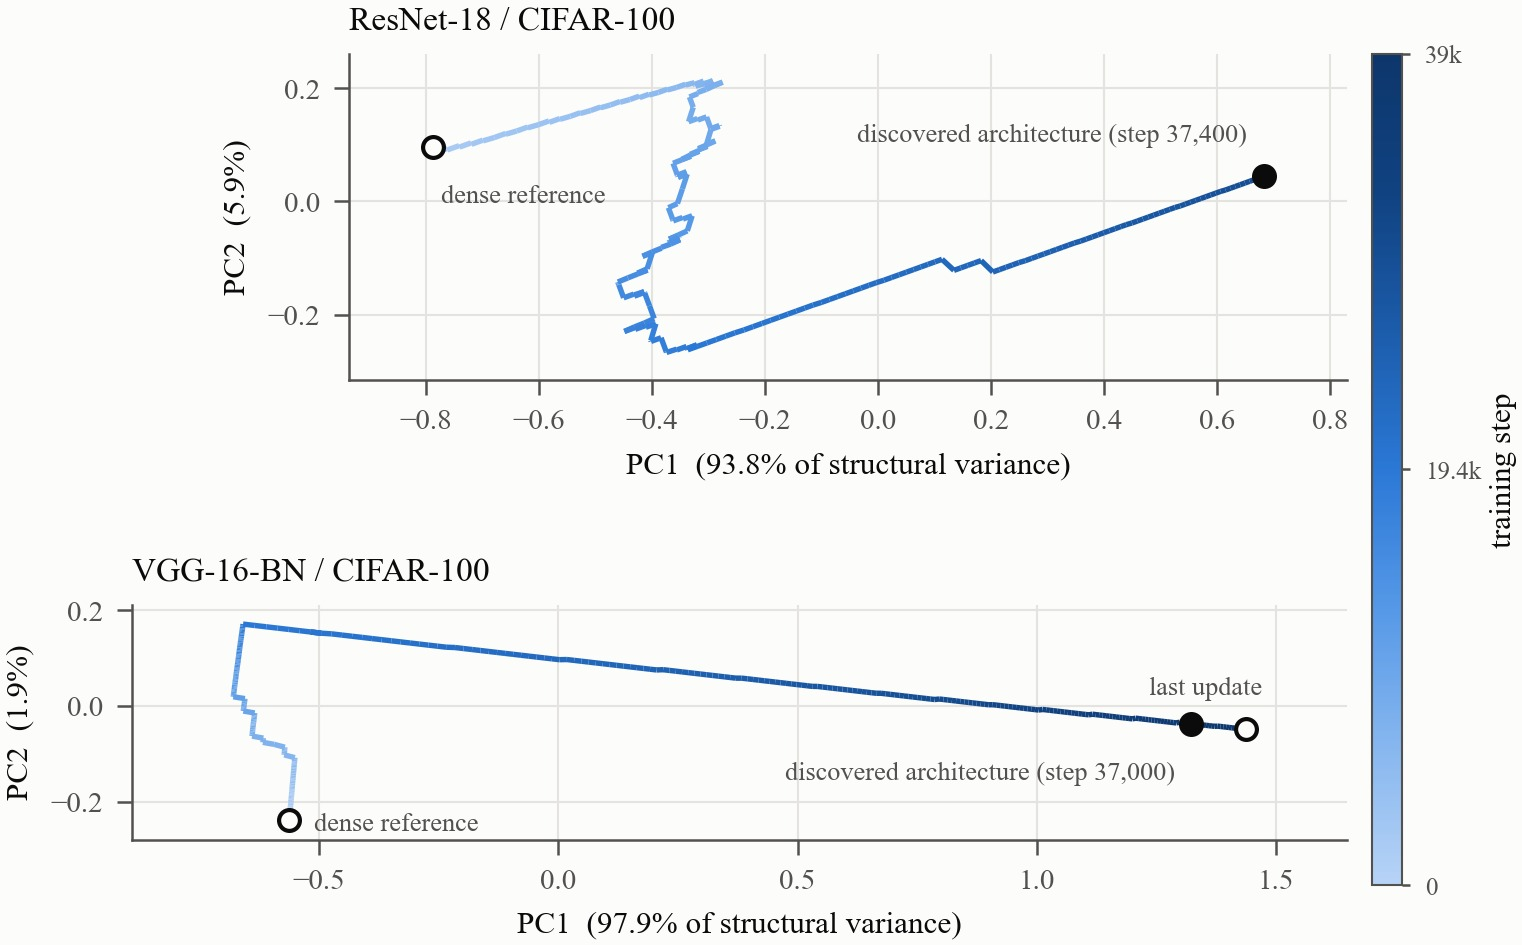
\includegraphics[width=\textwidth]{figures/appendix_pair_architecture_path.jpg}
\caption{The path through width space, in each run's first two principal components, on equal axes and colored by training step. ResNet-18 (top) carries $93.8\%$ of its structural variance on PC1; the path wanders while the ceiling is falling and then moves in a straight line once it settles. VGG-16-BN (bottom) carries $97.9\%$ on PC1, and its anneal phase barely leaves the neighborhood of the reference. The filled marker is the exported architecture; where the run continued past it, the open marker is the last logged update. The components describe these two trajectories, not a general basis.}
\label{fig:cs-path}
\end{figure}

\begin{figure}[htbp]
\centering
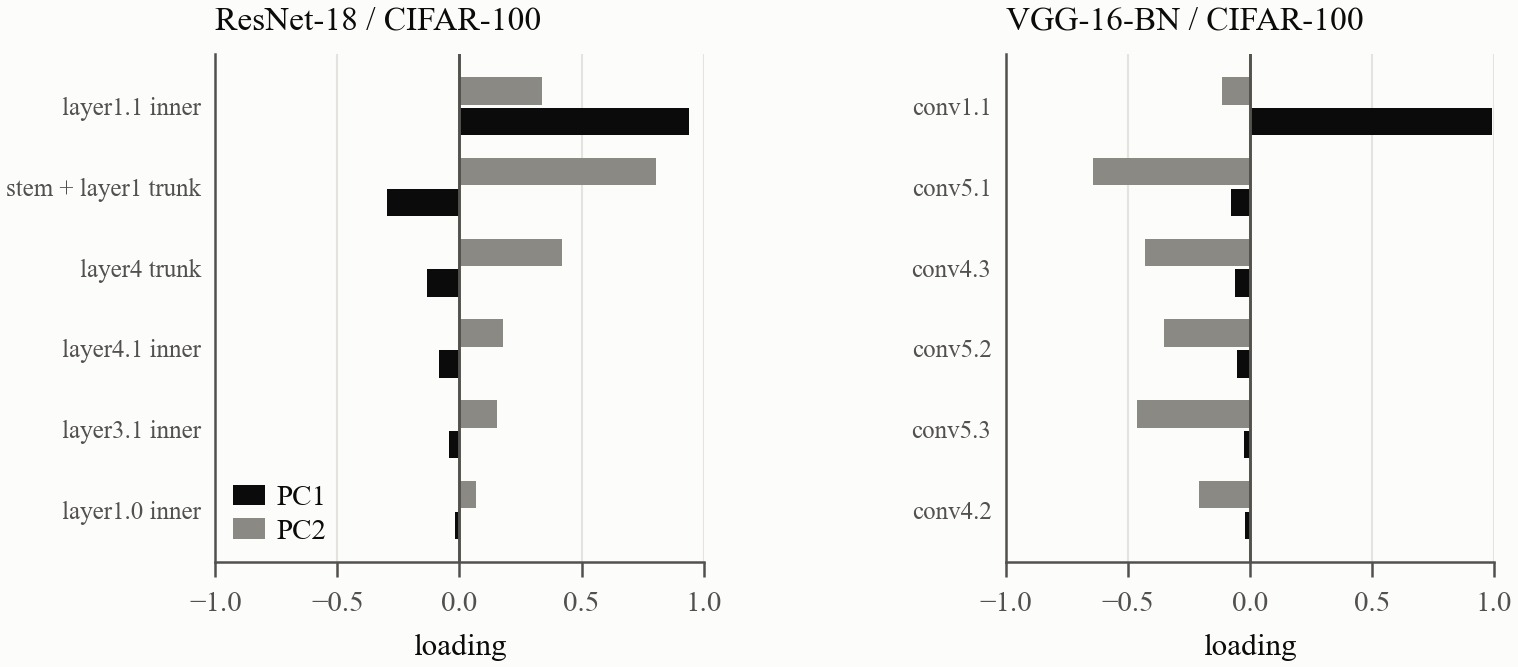
\includegraphics[width=\textwidth]{figures/appendix_pair_architecture_loadings.jpg}
\caption{What the principal axes are made of: loadings of the six groups with the largest $|\mathrm{PC1}|$. In both runs PC1 is a single site set against the deep groups: layer1.1's inner width ($+0.94$) against the stem/layer1 trunk ($-0.30$) and the layer4 trunk ($-0.13$) for ResNet-18; conv1.1 ($+0.99$) against the block-4 and block-5 convolutions for VGG-16-BN. To first order each discovery is one transfer, from the deep, expensive groups to one early, cheap one.}
\label{fig:cs-loadings}
\end{figure}

\begin{figure}[htbp]
\centering
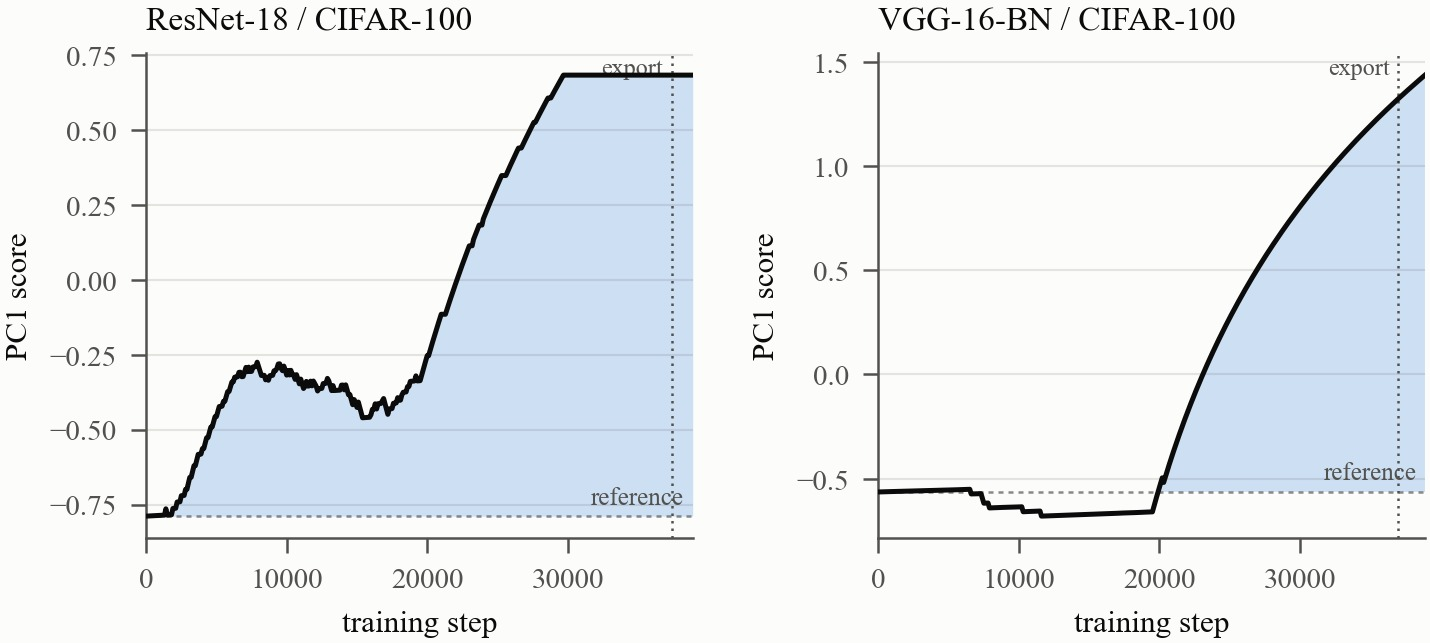
\includegraphics[width=\textwidth]{figures/appendix_pair_architecture_pc1.jpg}
\caption{The dominant coordinate over training; the dotted line marks the export step. ResNet-18 climbs in two stages, stalling and partly reversing while the ceiling is still falling and resuming once it settles. VGG-16-BN is flat until the ceiling reaches its target at step 19,500 and then rises monotonically, still rising when training ends.}
\label{fig:cs-pc1}
\end{figure}

\subsection{Where the edits went}

\begin{figure}[htbp]
\centering
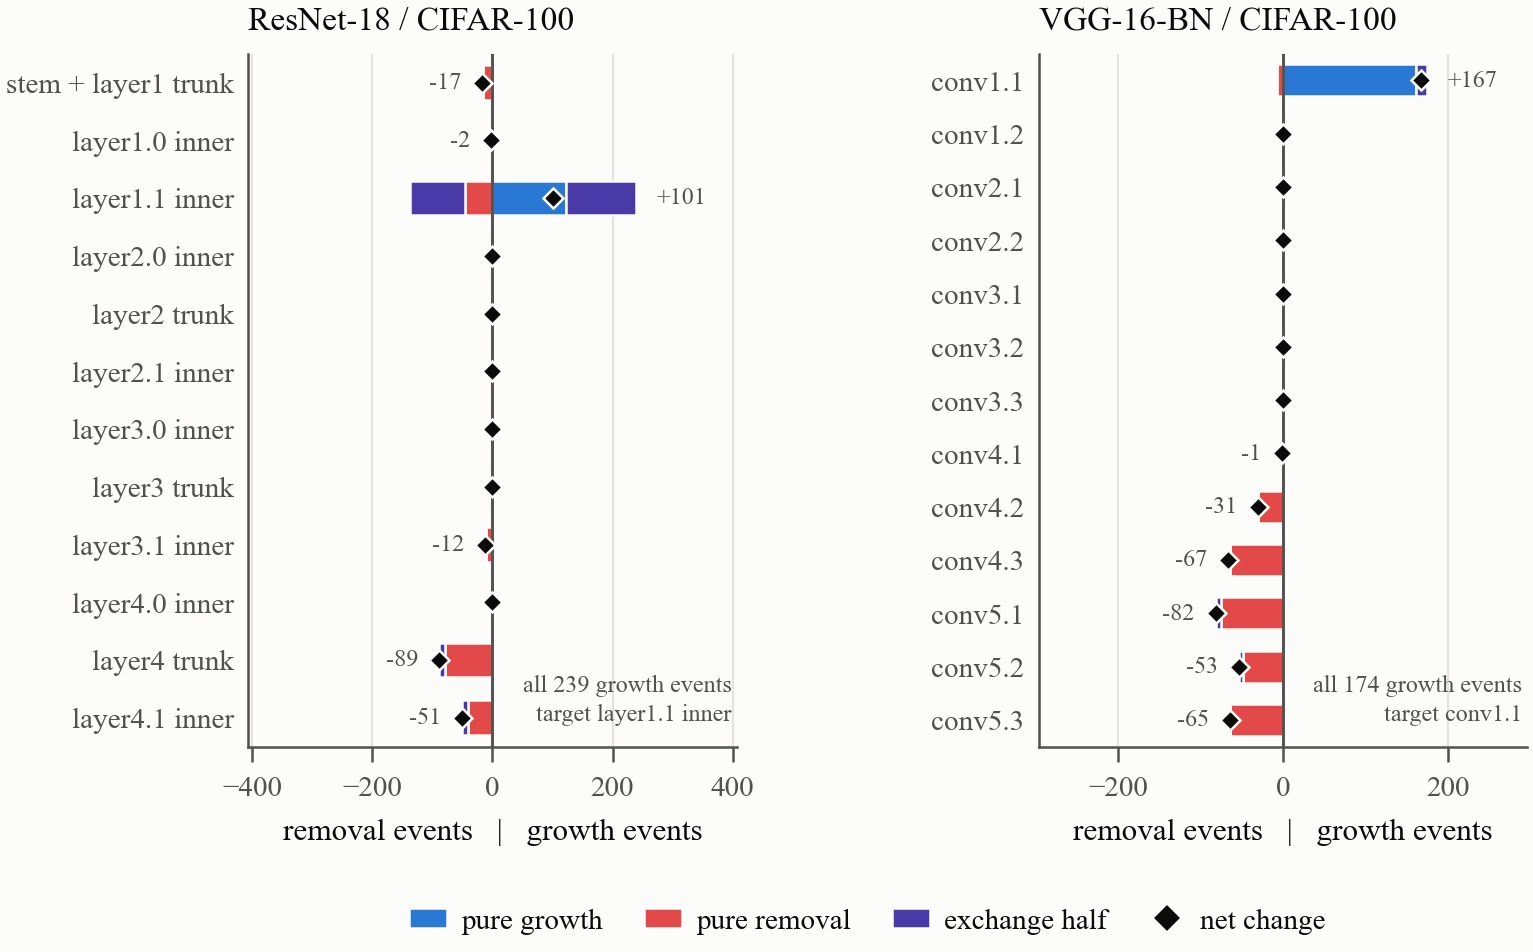
\includegraphics[width=\textwidth]{figures/appendix_pair_edit_counts.jpg}
\caption{Edits per coupling group up to the exported checkpoint: removals to the left of zero, growth to the right, split into pure edits and the two halves of an exchange; the marker is the net width change. Every growth event in both runs targets a single group, 239 at layer1.1's inner width and 174 at conv1.1, and in ResNet-18 that group is also its most-pruned site (138 removals), consistent with the absence of a newborn-protection interval in the released controller (\cref{app:materialization}). ResNet-18 exchanges freely (132 up to export); VGG-16-BN almost never does (13), moving capacity through pure removals during the anneal and pure growths after it.}
\label{fig:cs-edit-counts}
\end{figure}

\begin{figure}[htbp]
\centering
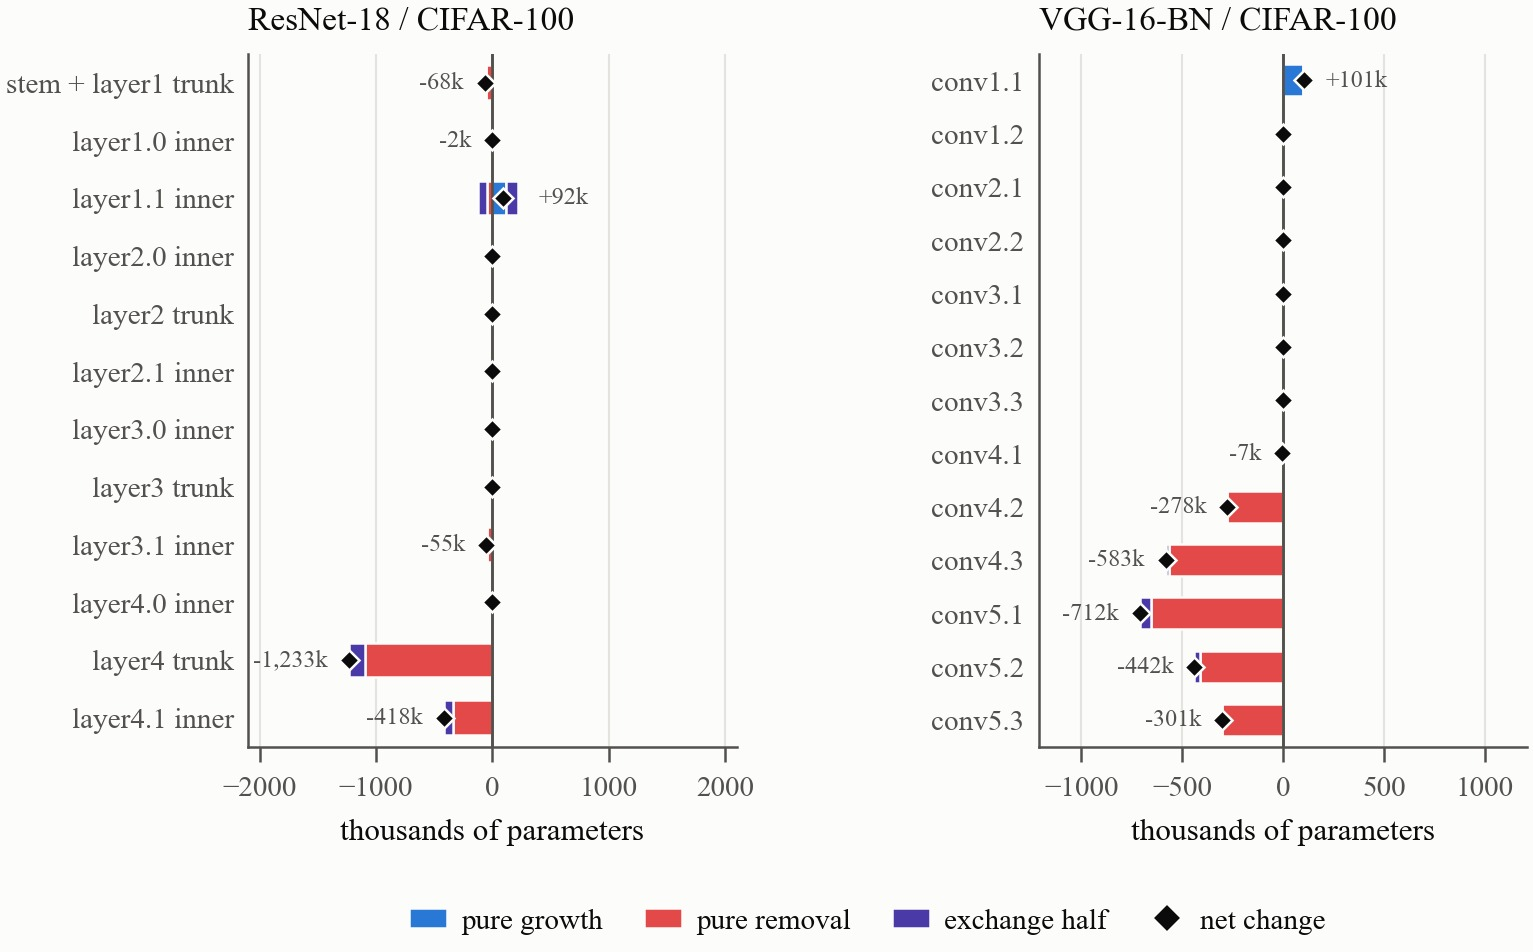
\includegraphics[width=\textwidth]{figures/appendix_pair_edit_params.jpg}
\caption{The same edits weighted by the exact parameter cost of the index moved. One channel costs 1,154 parameters at layer1.1 and 13,970 at the layer4 trunk of ResNet-18; 606 at conv1.1 and 9,201 at conv5.1 of VGG-16-BN. Counts and parameters therefore disagree: the growth site receives the most events but a small share of the parameters, and the reduction is paid almost entirely by the deep, wide groups ($-1.23$M at the layer4 trunk, $-712$k at conv5.1). Event counts are not a proxy for capacity moved.}
\label{fig:cs-edit-params}
\end{figure}

\subsection{The controller's signals over training}

The log records, for each window, the candidate the controller selected and the incumbent it removed, so the points below are the accepted edits, not the population they were chosen from. Shading spans the updates that entered the feasibility regime.

\begin{figure}[htbp]
\centering
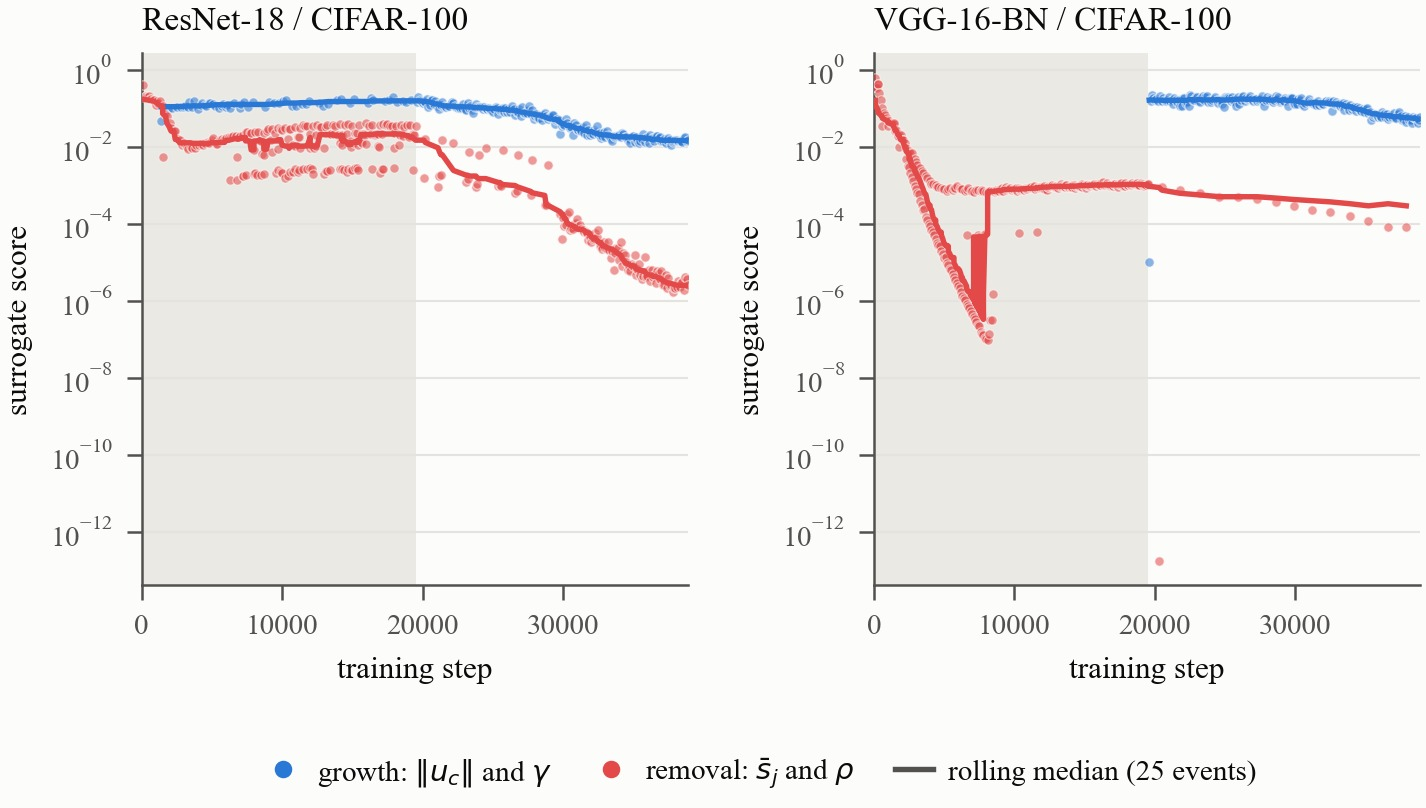
\includegraphics[width=\textwidth]{figures/appendix_pair_signal_score.jpg}
\caption{The surrogate score of each accepted edit against training step, with a rolling median over 25 events per side. The removal score $\bar s_j$ falls about four decades in ResNet-18 and two in VGG-16-BN as the inner problem converges, which is why the released controller's pure-removal test is relative to each group's own median rather than an absolute floor (\cref{eq:relativeprune}): any fixed threshold is eventually crossed by every channel.}
\label{fig:cs-signal-score}
\end{figure}

\begin{figure}[htbp]
\centering
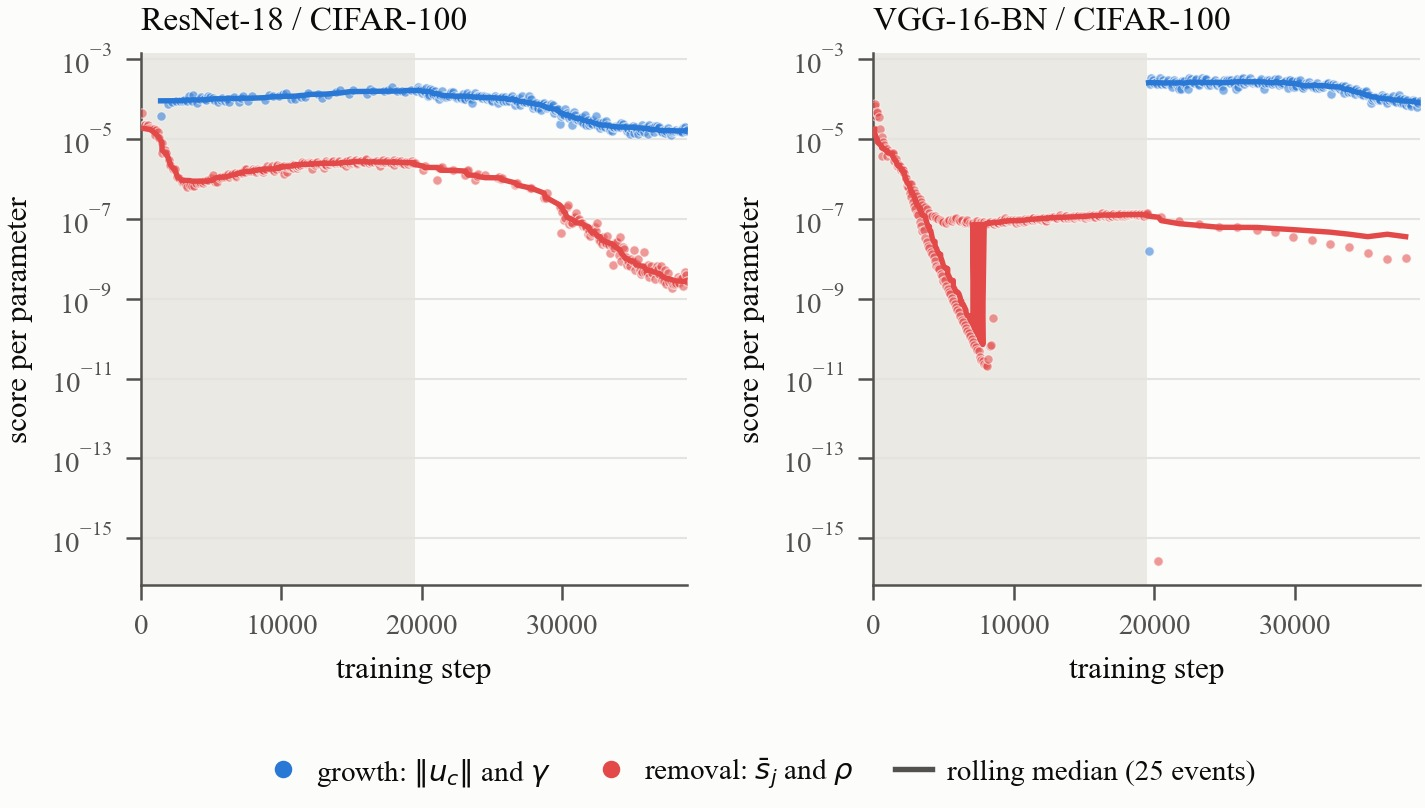
\includegraphics[width=\textwidth]{figures/appendix_pair_signal_density.jpg}
\caption{The same edits as densities, score per parameter of the index moved, which is the quantity the controller ranks by. The growth density it accepts sits far above the removal density it pays throughout: the median ratio $\gamma/\rho$ over accepted exchanges is about 650 in ResNet-18 (132 exchanges) and about 6,000 in VGG-16-BN (14), and in both runs the gap widens rather than closing. Neither run approaches the equimarginal condition of \cref{thm:equimarginal}; both stop because training ends.}
\label{fig:cs-signal-density}
\end{figure}

\subsection{Score against cost}

\begin{figure}[htbp]
\centering
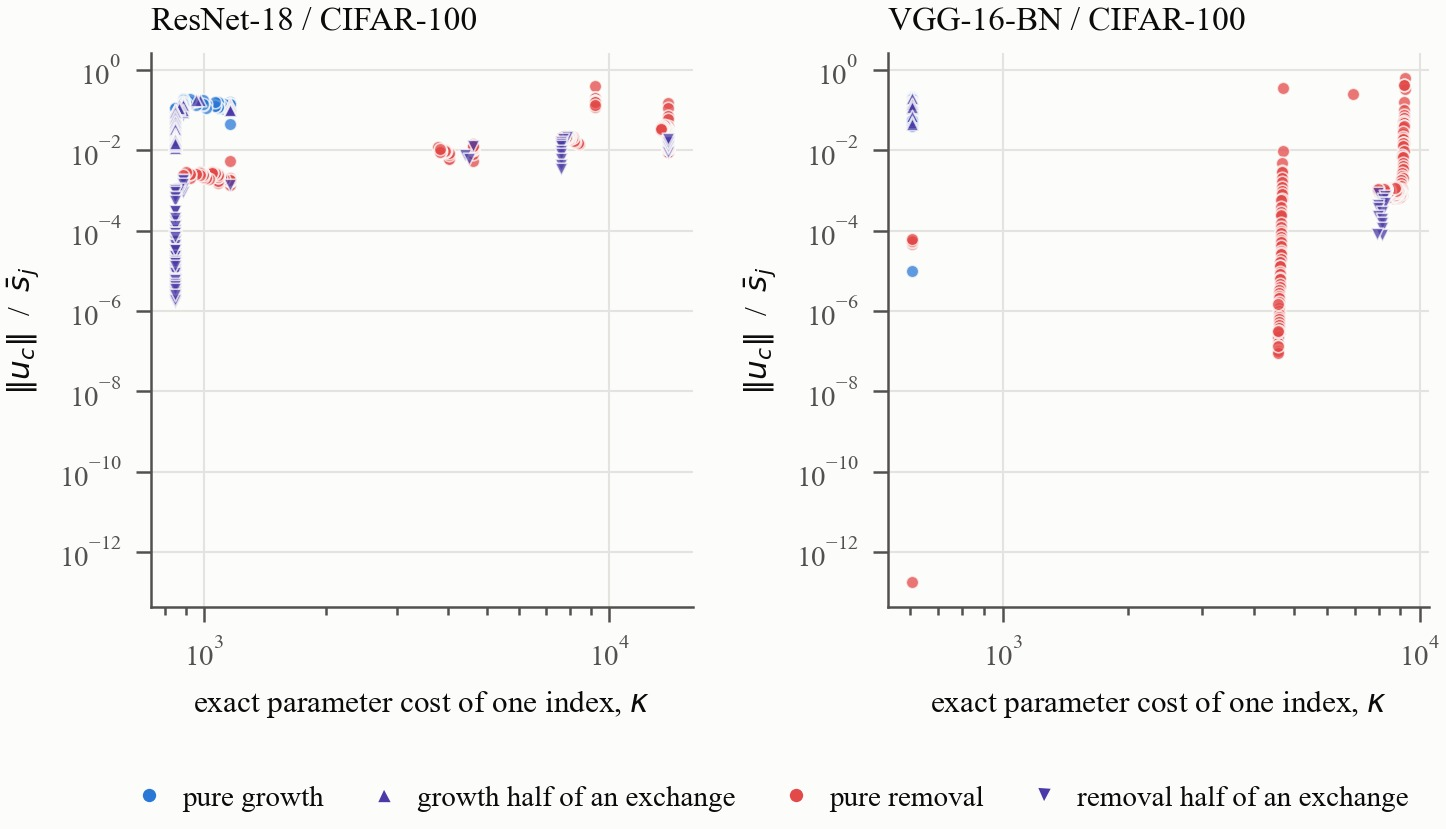
\includegraphics[width=\textwidth]{figures/appendix_pair_score_cost_raw.jpg}
\caption{Surrogate score against the exact parameter cost of the index moved, for accepted edits. Growth signals $\|u_c\|$ and removal scores $\bar s_j$ share an axis because Case C compares them directly; they remain surrogates in different units, not commensurable loss changes. In VGG-16-BN the costs separate into two clusters an order of magnitude apart, the 606-parameter channels of conv1.1 where every growth lands and the several-thousand-parameter channels of blocks 4 and 5 where nearly every removal lands; ResNet-18's costs spread over the same range with its exchanges concentrated at the cheap end.}
\label{fig:cs-score-raw}
\end{figure}

\begin{figure}[htbp]
\centering
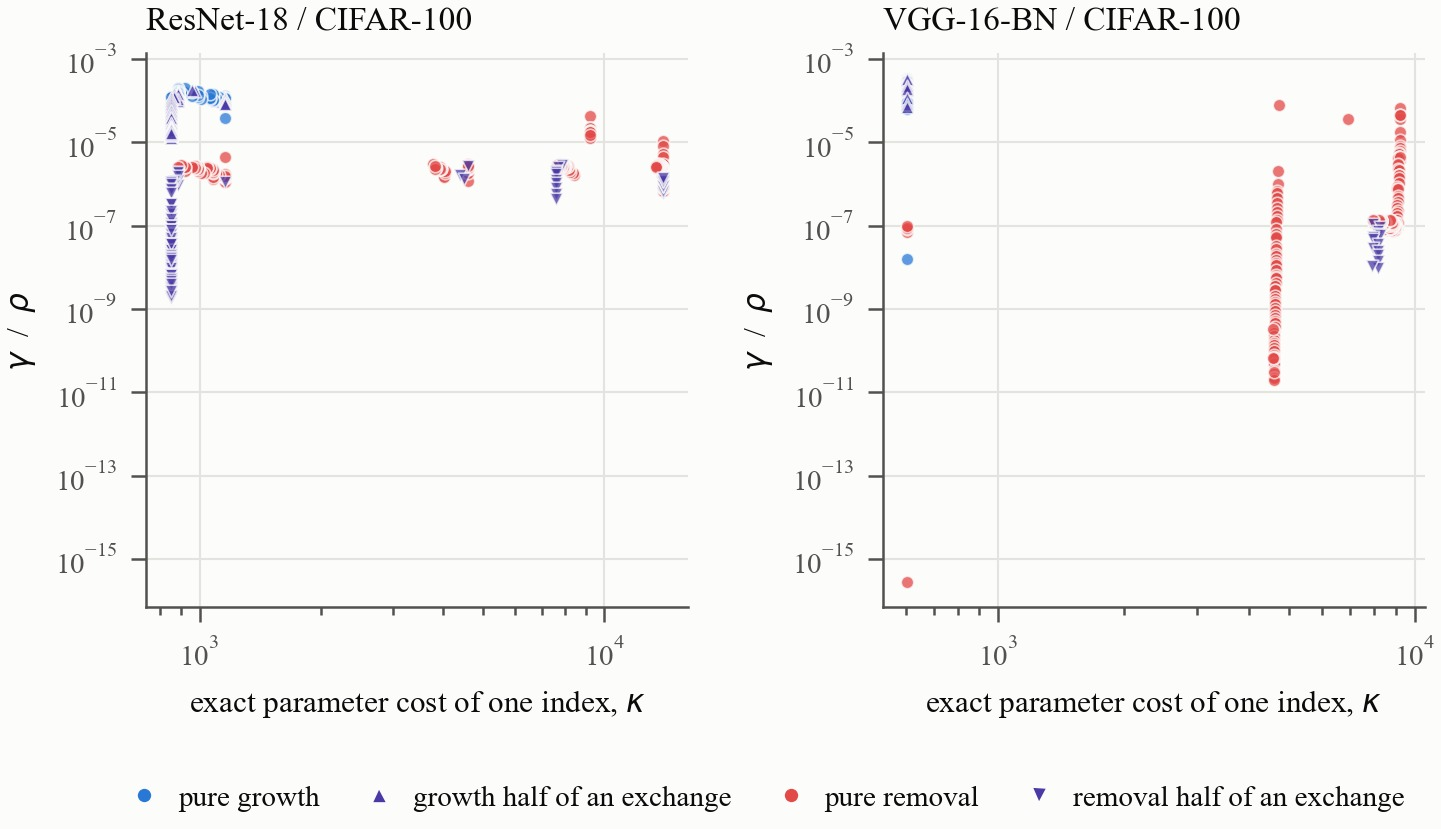
\includegraphics[width=\textwidth]{figures/appendix_pair_score_cost_density.jpg}
\caption{Score per parameter against cost. Dividing by cost lifts the cheap site's edits and lowers the expensive sites', which is the asymmetry the exchange rule ranks on: in both runs the accepted growths sit at the low-cost end and above the accepted removals. Accepted edits only.}
\label{fig:cs-score-density}
\end{figure}

\subsection{What the three arms represent}

The figures above describe where capacity sits. The last two ask what the networks holding that capacity compute, by running the same 2,048 CIFAR-100 test images through the dense reference, the static-matched arm (C2) and the online arm, and comparing their hidden representations at probed stages, with spatial locations treated as samples. One seed per arm; the two matched arms share widths but not an initialization, so similarity below one between them includes ordinary seed-to-seed variation and is not by itself evidence that plasticity changed the representation.

\begin{figure}[htbp]
\centering
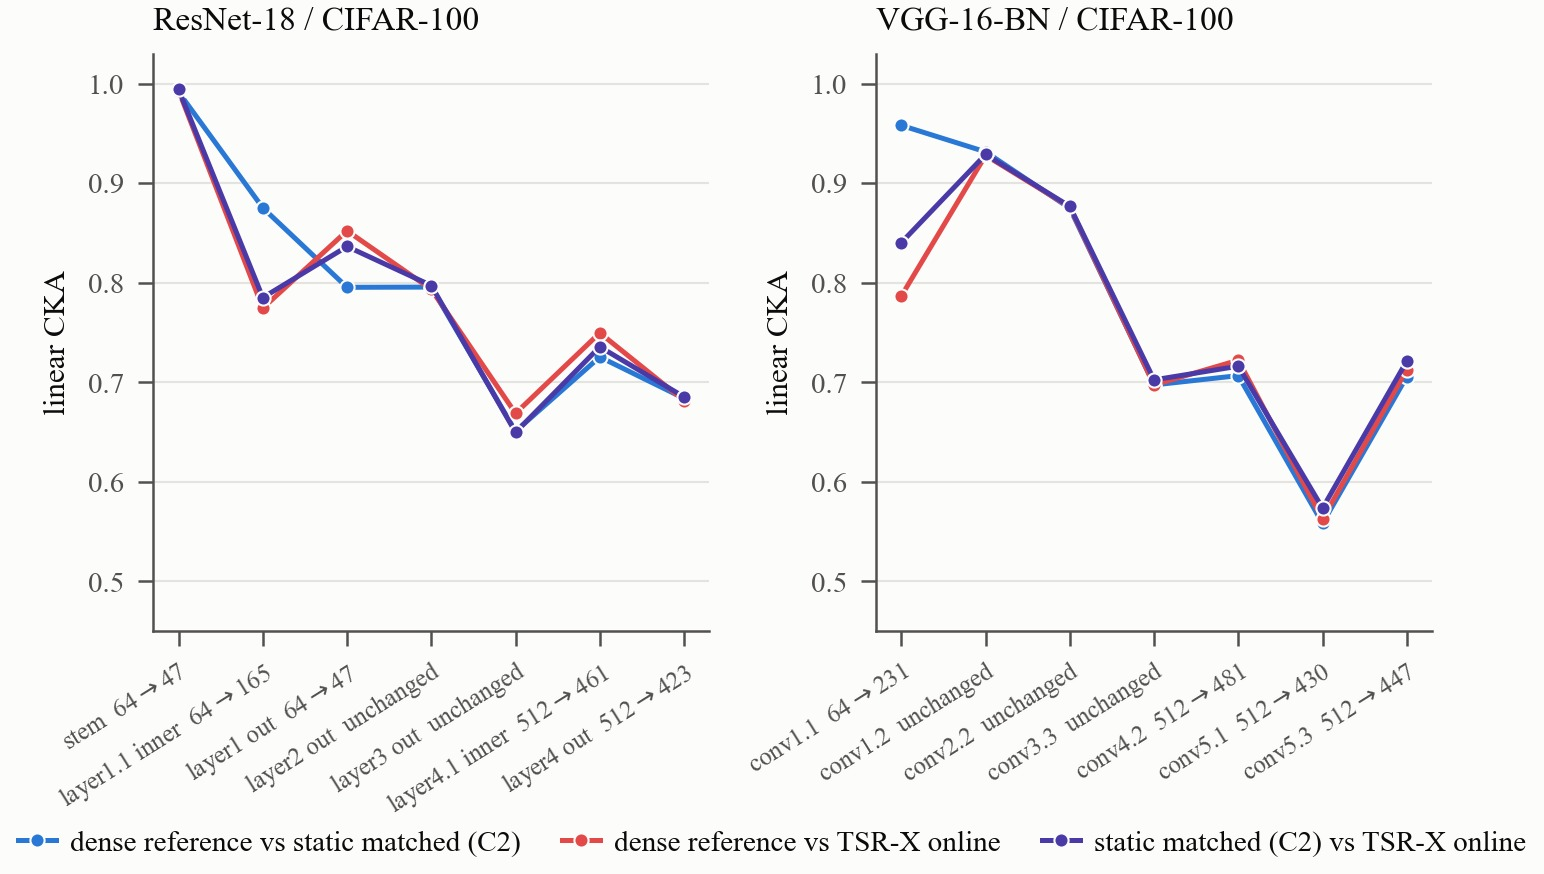
\includegraphics[width=\textwidth]{figures/appendix_pair_representation_cka.jpg}
\caption{Linear CKA \citep{kornblith2019similarity} between the three arms at each probed stage; the tick labels give the stage's reference $\rightarrow$ exported width. CKA is invariant to the width of the representations compared, which is what makes arms with different channel counts comparable. Similarity falls with depth in both runs and is lowest at the most-pruned deep stage of VGG-16-BN (conv5.1, $0.56$ to $0.57$), but the reference-vs-C2 pair is as far apart there as the pairs involving the online arm, so that divergence is seed variation at least as much as it is pruning.}
\label{fig:cs-cka}
\end{figure}

\begin{figure}[htbp]
\centering
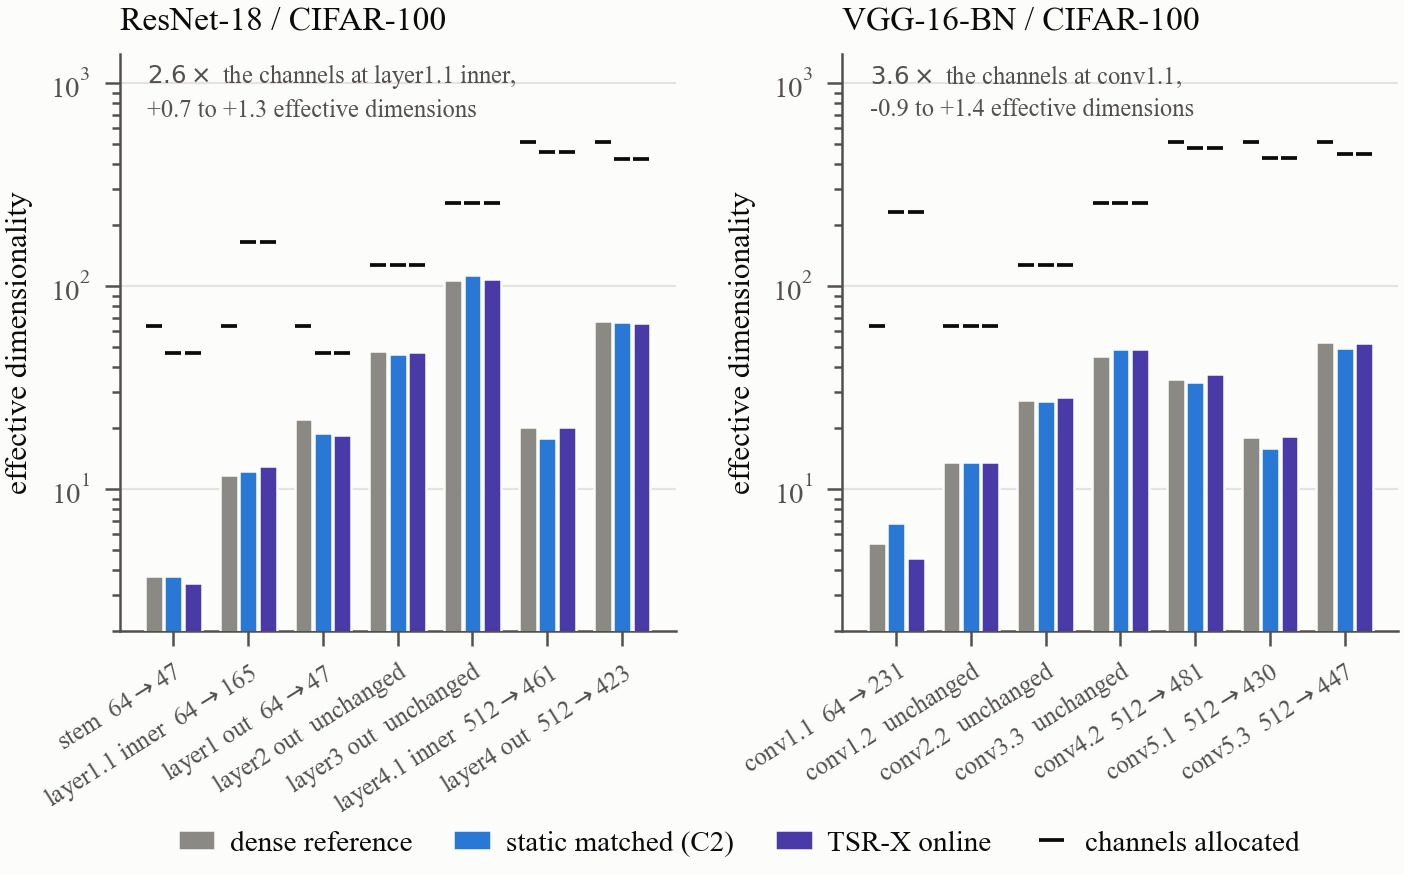
\includegraphics[width=\textwidth]{figures/appendix_pair_representation_dimensionality.jpg}
\caption{Effective dimensionality (participation ratio of the feature covariance spectrum, \citealp{gao2017theory}) of each arm at the same stages, against the channels allocated (dashes). Every stage uses a small fraction of its width: layer4.1's inner width spans about 20 dimensions across 512 channels and conv5.1 about 18, which is the empirical form of the redundancy the reduction exploits. The grown sites are no exception. $2.6\times$ the channels at layer1.1 bought $+0.7$ to $+1.3$ effective dimensions; $3.6\times$ at conv1.1 bought $-0.9$ to $+1.4$.}
\label{fig:cs-dimensionality}
\end{figure}

\clearpage

\end{document}
